\documentclass{cskkuproject}

% ==========================================
% ข้อมูลโครงงาน — ตัวอย่างประเภท A: พัฒนาระบบ
% ==========================================

\titleTH{การออกแบบและพัฒนาเกมเดินเรือด้วยระบบสั่งการด้วยเสียงเพื่อส่งเสริมทักษะการสื่อสาร}
\titleEN{Design and Development of a Voice-Controlled Ship Navigation Game to Enhance Communication Skills}

% ข้อมูลนักศึกษาคนที่ 1
\firstStudentID{663380213-6}
\firstStudentPrefixTH{นาย}
\firstStudentPrefixEN{Mr.}
\firstStudentNameTH{ธิติวุฒิ ศรีอมรรัตน์}
\firstStudentNameEN{Thitiwut Sriamonrat}

% ข้อมูลหลักสูตร
\degreeTH{วิทยาศาสตรบัณฑิต}
\degreeEN{Bachelor of Science}
\majorTH{วิทยาการคอมพิวเตอร์}
\majorEN{Computer Science}

% อาจารย์ที่ปรึกษา
\advisorTH{ผศ.ดร.วชิราวุธ ธรรมวิเศษ}
\advisorEN{Asst. Prof. Wachirawut Thamviset, Ph.D.}

% ปีการศึกษา
\academicYearTH{2569}
\academicYearEN{2026}

% รหัสวิชา
\courseCode{CP354 771}
\courseName{โครงงานทางวิทยาการคอมพิวเตอร์}
\semester{2}

% คำสำคัญ
\keywordsTH{เกมเพื่อการเรียนรู้, การรู้จำเสียง, ความวิตกกังวลในการใช้ภาษาต่างประเทศ, การเรียนรู้โดยใช้เกมเป็นฐาน, เกมเดินเรือ}
\keywordsEN{Serious game, Speech recognition, Foreign language anxiety, Digital game-based learning, Ship navigation game}


% ตารางทุกตารางใช้คอลัมน์ L: ข้อความชิดซ้าย ไม่ยืดช่องว่างระหว่างคำภาษาไทยในคอลัมน์แคบ
\usepackage{array}
\newcolumntype{L}[1]{>{\raggedright\arraybackslash\hspace{0pt}}p{#1}}

% ช่องว่างระหว่างคำไทยที่ไม่มีเว้นวรรคในต้นฉบับยืดได้น้อยลง (เดิม plus 1pt)
% เพื่อไม่ให้คำในประโยคเดียวกันถูกแยกห่าง เช่น "การ เรียน รู้"
\XeTeXlinebreakskip = 0pt plus 0.2pt

% รายการข้อในคอลัมน์ที่ย่อเข้ามา: ยอมให้ขอบขวาไม่เสมอได้เล็กน้อย แทนการยืดช่องว่างระหว่างคำ
% (LaTeX ตั้ง \rightskip ของรายการจาก \@rightskip จึงต้องตั้งทั้งสองค่า)
\makeatletter
\newcommand{\listraggedright}{\@rightskip=0pt plus 2em\relax\rightskip=\@rightskip}
\makeatother
\setlist{before=\listraggedright}

% เนื้อหาย่อหน้า: ยอมให้ขอบขวาสั้นลงได้ไม่เกินประมาณ 1 ตัวอักษร แทนการยืดช่องว่างจนเห็นเป็นช่องโหว่
\makeatletter
\AtBeginDocument{\@rightskip=0pt plus 1em\relax\rightskip=\@rightskip}
\makeatother

% หัวข้อชิดซ้ายและไม่ตัดคำด้วยยัติภังค์ (รูปแบบอื่นเหมือนเทมเพลต)
\newcommand{\headingstyle}{\bfseries\large\upshape\raggedright\hyphenpenalty=10000\exhyphenpenalty=10000}
\titleformat{\section}{\headingstyle}{\thesection}{0.45\firstindentlength}{}
\titleformat{\subsection}{\headingstyle}{\thesubsection}{0.45\firstindentlength}{}
\titleformat{\subsubsection}{\headingstyle}{\thesubsubsection}{0.45\firstindentlength}{}
\titleformat{name=\section,numberless}{\headingstyle}{}{0pt}{}
\titleformat{name=\subsection,numberless}{\headingstyle}{}{0pt}{}
\titleformat{name=\subsubsection,numberless}{\headingstyle}{}{0pt}{}

% ตารางและรูปวางในตำแหน่งที่เหมาะ (ไม่บังคับ [H]) เพื่อไม่ให้เหลือที่ว่างครึ่งหน้า
% แต่ไม่ลอยข้ามหัวข้อ \section
\usepackage[section]{placeins}
% หน้าที่มีแต่ตาราง/รูป: เริ่มจากบนหน้า ไม่จัดกึ่งกลางแนวตั้ง และให้ตาราง/รูปอยู่ร่วมกับข้อความได้มากขึ้น
\makeatletter
\setlength{\@fptop}{0pt}
\setlength{\@fpbot}{0pt plus 1fil}
\makeatother
\renewcommand{\topfraction}{0.9}
\renewcommand{\bottomfraction}{0.8}
\renewcommand{\textfraction}{0.07}
\renewcommand{\floatpagefraction}{0.75}
\setcounter{topnumber}{3}
\setcounter{totalnumber}{4}

% คำบรรยายภาพที่ยาวเกิน 1 บรรทัด: ชิดซ้ายและไม่ตัดคำด้วยยัติภังค์ (บรรทัดเดียวยังจัดกึ่งกลาง)
\DeclareCaptionFont{nohyphen}{\hyphenpenalty=10000\relax}
\captionsetup[figure]{justification=raggedright,singlelinecheck=true,font=nohyphen}

% สารบัญ สารบัญภาพ และสารบัญตาราง: รายการที่ยาวเกินบรรทัดชิดซ้าย ไม่ยืดช่องว่าง
\makeatletter
\renewcommand{\@tocrmarg}{2.55em plus 1fil}
\makeatother

\begin{document}

% ==========================================
% หน้าปก
% ==========================================
\maketitlepage

% ตั้งค่าเลขหน้าส่วนต้นเป็นอักษรไทย (ก, ข, ค, ...)
\pagenumbering{arabic}
\setcounter{page}{0}
\renewcommand{\thepage}{\ThaiAlph{\value{page}}}

% ==========================================
% บทคัดย่อ
% ==========================================
\begin{abstractTH}
% บทคัดย่อภาษาไทย
โครงงานฉบับนี้มีวัตถุประสงค์เพื่อออกแบบและพัฒนาเกมเดินเรือด้วยระบบสั่งการด้วยเสียง (Voice-Controlled Ship Navigation Game) สำหรับเป็นสื่อการเรียนรู้เพื่อส่งเสริมทักษะการสื่อสารและลดความวิตกกังวลในการใช้ภาษาต่างประเทศของผู้เรียน โดยระบบผสมผสานรูปแบบเกมจำลองสถานการณ์เข้ากับเทคโนโลยีการรู้จำเสียง (Speech Recognition) ประกอบด้วยระบบหลัก ได้แก่ ระบบรู้จำเสียงและประมวลผลคำสั่ง ระบบฟิสิกส์และการควบคุมเรือ ระบบลูกเรือปัญญาประดิษฐ์ ระบบสร้างสิ่งกีดขวาง ระบบส่วนติดต่อผู้ใช้ ระบบช่วยสอนภาษา โหมดเนื้อเรื่อง และระบบบันทึกผลการทดลอง ผู้เล่นรับบทเป็นกัปตันเรือที่ต้องสื่อสารและสั่งการลูกเรือปัญญาประดิษฐ์ ได้แก่ ต้นกลเรือผู้ควบคุมเครื่องยนต์ และพลถือท้ายและยามระวังหน้าผู้บังคับหางเสือและเฝ้าระวังสิ่งกีดขวาง ด้วยวลีสื่อสารมาตรฐานทางทะเล ระบบพัฒนาด้วยเอนจิน Unity และภาษา C\# ระบบแปลงคำสั่งเสียงภาษาอังกฤษเป็นข้อความภายในเครื่องของผู้เล่นด้วยโมเดล Whisper ผ่านไลบรารี whisper.cpp แล้วส่งให้ตัวแยกคำสั่งตีความ หากตัวแยกคำสั่งไม่เข้าใจคำสั่ง ระบบจึงใช้ GPT-4o mini ช่วยตีความ ระบบลูกเรือปัญญาประดิษฐ์จำลองสถานการณ์สื่อสารขัดข้องเมื่อผู้เล่นออกเสียงไม่ชัดเจนหรือใช้คำสั่งผิดบริบท โดยลูกเรือจะทวนถามหรือขอให้พูดซ้ำ เกมจึงออกแบบมาเพื่อให้ผู้เล่นได้ฝึกความคล่องแคล่วในการพูดและการแก้ปัญหาเฉพาะหน้าภายใต้ความกดดัน ในรายงานความก้าวหน้าครั้งนี้ ผู้จัดทำได้พัฒนาต้นแบบของเกมแล้ว ผ่านการทดสอบหน่วย (Unit Test) ครบทั้ง 363 จาก 363 กรณี และการทดสอบระบบโดยผู้จัดทำ ส่วนการประเมินกับผู้ใช้จะดำเนินการในระยะถัดไป โดยจะประเมินประสิทธิภาพของระบบจากแฟ้มบันทึกผลภายในเกม และเปรียบเทียบความวิตกกังวลในการพูดภาษาอังกฤษของกลุ่มตัวอย่างจำนวน 10--20 คนก่อนและหลังเล่นเกมด้วยแบบวัด 12 ข้อที่ดัดแปลงจาก Foreign Language Classroom Anxiety Scale (FLCAS) ร่วมกับแบบสอบถามประสบการณ์การเล่นเกม

\end{abstractTH}

\begin{abstractEN}
% ABSTRACT (English)
This project aims to design and develop a voice-controlled ship navigation game as a learning tool to enhance communication skills and reduce foreign language anxiety among learners. The system integrates a simulation game format with speech recognition technology and consists of the following main systems: the speech recognition and command processing system, the ship physics and control system, the AI crew system, the obstacle generation system, the user interface, the language support system, the story mode, and the research logging system. The player takes the role of a ship captain who must communicate with and issue standard marine orders to an AI crew, namely the chief engineer, who runs the engine, and the helmsman and lookout, who steers the ship and watches for hazards. The game is developed with the Unity engine and C\#. English voice commands are transcribed on the player's computer by the Whisper model via whisper.cpp; unclear commands are interpreted with GPT-4o mini. The AI crew system simulates communication breakdowns: if the player's pronunciation is unclear or a command is out of context, the crew asks the player to confirm or repeat the order. The game is therefore designed to give players practice in speaking fluently and solving problems under time pressure. At this progress stage, a working prototype has been built, all 363 of 363 unit tests pass, and the developer's own system tests have been completed; the user evaluation is planned for the next phase. The system's performance will be measured from in-game logs, and the speaking anxiety of 10--20 participants will be compared before and after play using a 12-item scale adapted from the Foreign Language Classroom Anxiety Scale (FLCAS), together with a game experience questionnaire.

\end{abstractEN}

% ==========================================
% กิตติกรรมประกาศ
% ==========================================
\begin{acknowledgement}
ข้าพเจ้าขอขอบพระคุณ ผศ.ดร.วชิราวุธ ธรรมวิเศษ อาจารย์ที่ปรึกษาโครงงาน
ที่ได้กรุณาให้คำแนะนำ คำปรึกษา และข้อเสนอแนะอันเป็นประโยชน์
รวมทั้งสละเวลาในการตรวจแก้ไข

ขอขอบพระคุณเพื่อนร่วมชั้นและผู้ที่เกี่ยวข้องทุกท่าน
ที่ได้ให้ความช่วยเหลือ แนะนำ และแลกเปลี่ยนความคิดเห็น
ซึ่งเป็นประโยชน์ต่อการดำเนินงานในหลายด้าน

ท้ายที่สุดนี้ ข้าพเจ้าขอขอบพระคุณบิดา มารดา และครอบครัว
ที่ให้การสนับสนุนและส่งเสริมตลอดระยะเวลาการศึกษา

\end{acknowledgement}

% ==========================================
% สารบัญ
% ==========================================
\tableofcontents
\clearpage
\listoffigures
\clearpage
\listoftables
\clearpage

% ==========================================
% เนื้อเรื่อง 5 บท
% ==========================================
\pagenumbering{arabic}
\setcounter{page}{1}

\chapter{บทนำ}
% =============================================================
% บทที่ 1 - บทนำ
% โครงงาน: การออกแบบและพัฒนาเกมเดินเรือด้วยระบบสั่งการด้วยเสียงเพื่อส่งเสริมทักษะการสื่อสาร
%          (Design and Development of a Voice-Controlled Ship Navigation Game to Enhance Communication Skills)
% =============================================================

% -----------------------------------------------------------
\section{ความเป็นมาและความสำคัญของปัญหา}
% -----------------------------------------------------------
ในปัจจุบัน ภาษาอังกฤษมีบทบาทสำคัญอย่างยิ่งในการเป็นเครื่องมือสื่อสารระดับสากล ทว่าการเรียนการสอนภาษาอังกฤษในห้องเรียนโดยทั่วไปยังคงเผชิญกับข้อจำกัดในการสร้างสภาพแวดล้อมที่เอื้อต่อการนำไปใช้งานจริง~\cite{sadigzade2025} ผู้เรียนจำนวนมากประสบปัญหาความวิตกกังวลในการใช้ภาษาต่างประเทศ (Foreign Language Anxiety) และกลัวความผิดพลาดเมื่อต้องเปล่งเสียงเพื่อสื่อสาร ส่งผลให้ขาดความมั่นใจและไม่สามารถเชื่อมโยงทักษะทางภาษาเข้ากับสถานการณ์ในชีวิตจริงหรือการโต้ตอบแบบทันท่วงทีได้~\cite{varma2025}
ที่ผ่านมา มีความพยายามนำสื่อดิจิทัลและเกมมาประยุกต์ใช้เพื่อการเรียนรู้ภาษา (Game-Based Language Learning) แต่ยังคงพบกับความท้าทายสำคัญ~\cite{sadigzade2025} งานวิจัยชี้ให้เห็นว่าแอปพลิเคชันหรือเกมเพื่อการเรียนรู้ภาษาแบบดั้งเดิมมักเน้นไวยากรณ์และการท่องจำคำศัพท์เป็นหลัก ทำให้รูปแบบการเล่นจำเจอยู่กับการคลิกเลือกคำตอบหรือการอ่านข้อความ ในขณะที่เกมที่เน้นความสนุกสนานก็มักไม่ได้กำหนดให้ผู้เล่นต้องเปล่งเสียงพูดออกมา~\cite{varma2025} ช่องว่างนี้แสดงให้เห็นถึงโอกาสในการสร้างสรรค์เกมที่สามารถบูรณาการการฝึกฝนทักษะการพูดเข้ากับบริบทที่น่าตื่นเต้นและท้าทาย เพื่อกระตุ้นให้เกิดการสื่อสารอย่างเป็นธรรมชาติ~\cite{zargham2024}
โครงงานการออกแบบและพัฒนาเกมเดินเรือด้วยระบบสั่งการด้วยเสียงเพื่อส่งเสริมทักษะการสื่อสารจึงจัดทำขึ้น เพื่อพัฒนาแนวทางการเรียนรู้ภาษาอังกฤษผ่านสภาพแวดล้อมแบบดื่มด่ำ (Immersive Environment) ผู้เล่นจะรับบทเป็น ``กัปตันเรือ'' ที่ต้องเผชิญกับสถานการณ์จำลองการเดินเรือฝ่าสภาพแวดล้อมที่ท้าทาย โดยภารกิจของผู้เล่นไม่ใช่เพียงการควบคุมทิศทางผ่านหน้าจอ แต่คือการใช้ ``เสียง'' เป็นเครื่องมือหลักในการสั่งการลูกเรือปัญญาประดิษฐ์ (AI Crew) ในตำแหน่งต่าง ๆ ได้แก่ ต้นกลเรือ (Chief Engineer) ผู้ควบคุมเครื่องยนต์และความเร็ว และพลถือท้ายและยามระวังหน้า (Helmsman and Lookout) ผู้บังคับหางเสือและเฝ้าระวังสิ่งกีดขวาง เพื่อบังคับเรือไม่ให้ชนสิ่งกีดขวางและนำเรือไปสู่เป้าหมายอย่างปลอดภัย โดยคำสั่งที่ใช้ในเกมยึดตามวลีสื่อสารมาตรฐานทางทะเลขององค์การทางทะเลระหว่างประเทศ (IMO Standard Marine Communication Phrases: SMCP)~\cite{imo2002smcp}

% -----------------------------------------------------------
\section{นิยามศัพท์เฉพาะ}
% -----------------------------------------------------------

\begin{enumerate}[label=\arabic*)]
    \item \textbf{เกมเพื่อการเรียนรู้ (Serious Game)} หมายถึง เกมที่ออกแบบโดยมีวัตถุประสงค์หลักเพื่อการเรียนรู้หรือการฝึกทักษะมากกว่าความบันเทิง
    \item \textbf{การรู้จำเสียง (Speech-to-Text / Speech Recognition)} หมายถึง เทคโนโลยีการแปลงคำสั่งเสียงพูดภาษาอังกฤษของผู้เล่นให้เป็นข้อความ เพื่อนำไปตรวจความถูกต้องและประมวลผลเป็นคำสั่งควบคุมเรือ
    \item \textbf{ตัวกรองทางอารมณ์ (Affective Filter)} หมายถึง อุปสรรคทางอารมณ์ เช่น ความกลัว ความวิตกกังวล และการขาดความมั่นใจ ซึ่งขัดขวางการเรียนรู้และการพูดภาษาที่สอง
    \item \textbf{ความวิตกกังวลในการใช้ภาษาต่างประเทศ} หมายถึง ความรู้สึกประหม่า กลัวการพูดผิด หรือกลัวการถูกประเมินในทางลบเมื่อต้องสื่อสารด้วยภาษาต่างประเทศ ในโครงงานนี้วัดด้วยแบบวัดความวิตกกังวลในการพูดภาษาอังกฤษที่ดัดแปลงจาก FLCAS
    \item \textbf{ลูกเรือปัญญาประดิษฐ์} หมายถึง ตัวละคร NPC (Non-Player Character) ในเกมที่รับคำสั่งเสียงจากผู้เล่นและให้เสียงตอบกลับ (Voice Feedback) เช่น การทวนคำสั่งหรือขอให้ย้ำคำสั่ง
    \item \textbf{สภาพแวดล้อมแบบดื่มด่ำ} หมายถึง สภาพแวดล้อมจำลองภายในเกมที่สร้างประสบการณ์การเรียนรู้ที่มีทั้งความท้าทาย ความสมจริง และความปลอดภัยทางความรู้สึก
\end{enumerate}

% -----------------------------------------------------------
\section{วัตถุประสงค์}
% -----------------------------------------------------------

\begin{enumerate}[label=\arabic*)]
    \item เพื่อออกแบบและพัฒนาเกมเดินเรือด้วยระบบสั่งการด้วยเสียง (Voice-Controlled Ship Navigation Game) สำหรับใช้เป็นสื่อการเรียนรู้แบบดื่มด่ำ (Immersive Learning) ที่มีความสมจริงและออกแบบเพื่อช่วยลดความวิตกกังวลในการใช้ภาษาต่างประเทศของผู้เรียน
    \item เพื่อประเมินประสิทธิภาพทางเทคนิคของระบบจากแฟ้มบันทึกผลในเกม ได้แก่ ความถูกต้องของการรู้จำคำสั่ง ร้อยละของการสื่อสารที่ลูกเรือเข้าใจ จำนวนครั้งที่ลูกเรือขอให้พูดซ้ำ และเวลาตอบสนอง และประเมินประสบการณ์การเล่นเกมของผู้เล่นด้วยแบบสอบถาม
    \item เพื่อเปรียบเทียบระดับความวิตกกังวลในการพูดภาษาอังกฤษของผู้เล่นก่อนและหลังการเล่นเกม โดยใช้แบบวัดที่ดัดแปลงจาก Foreign Language Classroom Anxiety Scale (FLCAS)
\end{enumerate}

% -----------------------------------------------------------
\section{เป้าหมายและขอบเขต}
% -----------------------------------------------------------

\subsection{ขอบเขตด้านเนื้อหา}

ระบบที่พัฒนาเป็นเกมแนวจำลองสถานการณ์ (Simulation Game) แบบผู้เล่นคนเดียว (Single-player) ที่ใช้เสียงเป็นช่องทางควบคุมหลัก ประกอบด้วยระบบหลัก ได้แก่

\begin{enumerate}[label=\arabic*)]
    \item \textbf{ระบบรู้จำเสียงและประมวลผลคำสั่ง (Speech Recognition \& Command Parser System):} ระบบรับเสียงจากไมโครโฟน แปลงเป็นข้อความ แล้วส่งให้ตัวแยกคำสั่ง (Command Parser) ตรวจสอบและแยกคำสั่งภาษาอังกฤษ
    \item \textbf{ระบบฟิสิกส์และการควบคุมเรือ (Ship Navigation Physics):} ระบบจำลองการเคลื่อนที่ของเรือที่มีความเฉื่อยและการตอบสนองต่อหางเสือที่สมจริง ทำให้ผู้เล่นต้องวางแผนล่วงหน้าในการออกคำสั่ง
    \item \textbf{ระบบลูกเรือปัญญาประดิษฐ์ (AI Crew System):} ระบบตัวละคร NPC ที่รับคำสั่งเสียงจากผู้เล่นและให้เสียงตอบกลับ เช่น การทวนคำสั่งเมื่อรับทราบ หรือการขอให้พูดซ้ำเมื่อไม่เข้าใจคำสั่ง
    \item \textbf{ระบบสร้างสิ่งกีดขวาง (Obstacle Generation System):} ระบบสร้างสิ่งกีดขวาง ได้แก่ หิน แนวหินโสโครก สันดอน และทุ่นระเบิด แบบสุ่มในเส้นทางการเดินเรือ ยกเว้นภารกิจโหมดเนื้อเรื่องซึ่งใช้แผนที่คงที่ เพื่อท้าทายให้ผู้เล่นต้องตัดสินใจออกคำสั่งหลบหลีกในทันที
    \item \textbf{ระบบส่วนติดต่อผู้ใช้ (UI/HUD):} หน้าจอแสดงข้อมูลที่จำเป็น เช่น เรดาร์ตรวจจับสิ่งกีดขวาง เข็มทิศแสดงองศาเรือ มาตรวัดความเร็ว และสัญลักษณ์แสดงสถานะการรับเสียงของไมโครโฟน
    \item \textbf{ระบบช่วยสอนภาษา (Language Support):} คำแนะนำประโยคที่ควรพูดในแต่ละสถานการณ์ การทวนคำสั่งของลูกเรือด้วยรูปประโยคมาตรฐาน และรายงานภาษาในหน้าสรุปผลเมื่อจบการเดินเรือ
    \item \textbf{โหมดเนื้อเรื่อง (Story Mode):} ภารกิจตามเนื้อเรื่อง 3 บท รวม 9 ภารกิจ
    \item \textbf{ระบบบันทึกผลการทดลอง (Research Log):} การบันทึกข้อมูลการเล่นลงแฟ้ม CSV แยกตามรอบการเปิดเกม เพื่อใช้วิเคราะห์ผล
\end{enumerate}

\subsection{ขอบเขตด้านประชากรและกลุ่มตัวอย่าง}

ประชากรคือนักศึกษาระดับปริญญาตรี กลุ่มตัวอย่างคืออาสาสมัครที่เลือกแบบสะดวก (Convenience Sampling) จำนวน 10--20 คน

\subsection{ขอบเขตด้านเทคนิค}

\begin{enumerate}[label=\arabic*)]
    \item พัฒนาตัวเกมด้วยเอนจิน Unity (Unity 6) และใช้ภาษา C\# สำหรับการพัฒนาสภาพแวดล้อมเกมและระบบฟิสิกส์ของการเดินเรือ
    \item นำเสนอภาพในรูปแบบมุมมองการเล่นแบบไอโซเมตริก (Isometric view) และรองรับการทำงานบนระบบปฏิบัติการ Windows PC
    \item ใช้ไมโครโฟนรับเสียงพูดภาษาอังกฤษเป็นช่องทางหลักในการสั่งการลูกเรือ โดยมีการพิมพ์คำสั่งผ่านแป้นพิมพ์เป็นช่องทางสำรอง ทั้งสองช่องทางผ่านขั้นตอนการประมวลผลคำสั่งเดียวกัน และไม่มีปุ่มบังคับหางเสือหรือคันโทรเลขเครื่องยนต์โดยตรง
    \item ใช้โมเดลการรู้จำเสียง Whisper ที่ทำงานภายในเครื่องของผู้เล่น (On-device) ผ่านไลบรารี whisper.cpp เพื่อแปลงเสียงพูดเป็นข้อความด้วยโมเดล ggml-base.en
    \item ใช้ API ของ OpenAI (โมเดล GPT-4o mini) เฉพาะเมื่อตัวแยกคำสั่งไม่เข้าใจคำสั่ง และเมื่อผู้เล่นสนทนากับลูกเรือ
\end{enumerate}

% -----------------------------------------------------------
\section{ประโยชน์ที่คาดว่าจะได้รับ}
% -----------------------------------------------------------

\begin{enumerate}[label=\arabic*)]
    \item ผู้เล่นได้ฝึกใช้วลีสั่งการมาตรฐานทางทะเลในสถานการณ์จำลอง
    \item ผู้เล่นมีความมั่นใจและกล้าพูดภาษาอังกฤษมากขึ้น
    \item ผู้สอนสามารถนำเกมไปใช้เป็นสื่อเสริมการเรียนการสอนเชิงปฏิบัติ
\end{enumerate}

\chapter{ทฤษฎีและงานวิจัยที่เกี่ยวข้อง}
% =============================================================
% บทที่ 2 - งานวิจัยและทฤษฎีที่เกี่ยวข้อง
% โครงงาน: การออกแบบและพัฒนาเกมเดินเรือด้วยระบบสั่งการด้วยเสียงเพื่อส่งเสริมทักษะการสื่อสาร
% =============================================================

% -----------------------------------------------------------
\section{งานวิจัย โครงงาน และระบบงานที่เกี่ยวข้อง}
% -----------------------------------------------------------

ในส่วนนี้นำเสนองานวิจัยและเกมที่มีลักษณะคล้ายคลึงกับโครงงานนี้ เพื่อศึกษาแนวคิด จุดเด่น และข้อจำกัด แล้วนำมาเป็นแนวทางในการออกแบบและพัฒนาระบบ

\subsection{การเรียนรู้ภาษาผ่านเกมด้วยเทคโนโลยีการประมวลผลภาษาธรรมชาติ}

งานวิจัยของ Sadigzade~\cite{sadigzade2025} นำเสนอการใช้เกมดิจิทัลร่วมกับเทคโนโลยีการรู้จำเสียงและการประมวลผลภาษาธรรมชาติ เพื่อสนับสนุนการเรียนรู้ภาษาอังกฤษ การให้ผู้เรียนได้โต้ตอบด้วยเสียงกับตัวละครปัญญาประดิษฐ์ภายในเกมช่วยสร้างสภาพแวดล้อมจำลองที่สมจริง ผลการศึกษาพบว่าช่วยเพิ่มแรงจูงใจ ลดความวิตกกังวลในการพูด และพัฒนาความคล่องแคล่วในการสื่อสารได้อย่างมีประสิทธิภาพ อย่างไรก็ตาม เกมในลักษณะดังกล่าวมักไม่ได้เน้นความกดดันด้านเวลาหรือสถานการณ์จำลองที่ต้องใช้ไหวพริบอย่างรวดเร็ว

\subsection{เครื่องมือเกมควบคุมด้วยเสียงเพื่อเสริมสร้างการเรียนรู้}

งานวิจัยของ Varma และคณะ~\cite{varma2025} มุ่งเน้นพัฒนาเกมที่ควบคุมการทำงานด้วยคำสั่งเสียงแบบเรียลไทม์ โดยทำงานผ่านการแปลงเสียงพูดเป็นคำสั่งเพื่อควบคุมการเคลื่อนที่ขององค์ประกอบในเกมแทนการใช้อุปกรณ์ควบคุมทั่วไป การควบคุมผ่านเสียงช่วยกระตุ้นให้ผู้เล่นต้องคิดตัดสินใจอย่างรวดเร็วและเปล่งเสียงให้ชัดเจน ซึ่งช่วยพัฒนาทักษะการตอบสนองได้ดี

\subsection{การสำรวจการโต้ตอบด้วยเสียงกับตัวละคร NPC ในเกม}

Zargham และคณะ~\cite{zargham2024} ได้สำรวจความคิดเห็นของผู้เชี่ยวชาญเกี่ยวกับการใช้เสียงพูดเพื่อสื่อสารกับตัวละคร NPC ในวิดีโอเกม ผลการวิจัยระบุว่าการสั่งการด้วยเสียงช่วยเพิ่มความรู้สึกดื่มด่ำ (Immersion) และความสมจริง นอกจากนี้ การให้ NPC ตอบสนองต่อคำสั่งเสียงอย่างเป็นธรรมชาติยังช่วยเพิ่มความผูกพันได้ แต่จำเป็นต้องคำนึงถึงบริบทและความแม่นยำของระบบรู้จำเสียงเพื่อป้องกันความหงุดหงิดจากการแปลความหมายผิดพลาด

\subsection{เกมเชิงพาณิชย์ที่สั่งการด้วยเสียง}

ในอุตสาหกรรมเกมเชิงพาณิชย์ มีการนำระบบรู้จำเสียงมาใช้ในเกมแนวจำลองสถานการณ์ (Simulation) เช่น เกม Powerboat VR~\cite{powerboat2020} ซึ่งผู้ผลิตเกมระบุว่าผู้เล่นสามารถใช้คำสั่งเสียงในการควบคุมเรือแทนอุปกรณ์ควบคุมทั่วไป และเกม Tower! 3D~\cite{tower3d2017} ที่ผู้เล่นรับบทผู้ควบคุมการจราจรทางอากาศและใช้เสียงพูดตามมาตรฐานคำศัพท์การบินเพื่อสั่งการเครื่องบิน นอกจากเกมจำลองสถานการณ์แล้ว ยังมีเกมแนวผจญภัย เช่น In Verbis Virtus~\cite{inverbis2015} ที่ผู้เล่นร่ายเวทมนตร์ด้วยการพูดคาถาผ่านไมโครโฟน เกมเหล่านี้แสดงให้เห็นว่าการสั่งการด้วยเสียงสามารถนำมาใช้เป็นกลไกหลักของเกมได้ แต่ไม่ได้ออกแบบมาเพื่อการฝึกภาษาหรือลดความวิตกกังวลในการพูด

\subsection{สรุปเปรียบเทียบงานวิจัยและเกมที่เกี่ยวข้อง}

จากการทบทวนระบบและงานวิจัยข้างต้น สามารถสรุปเปรียบเทียบคุณสมบัติหลักได้ดังตารางที่ \ref{tab:compare_research}

\begin{table}[!htbp]
\centering
\caption{เปรียบเทียบคุณสมบัติของระบบและเกมที่เกี่ยวข้อง}
\label{tab:compare_research}
\begin{tabular}{|L{3.50cm}|L{2.00cm}|L{2.00cm}|L{2.00cm}|L{2.00cm}|}
\hline
\textbf{ระบบ/เกม} & \textbf{ควบคุมด้วยเสียง} & \textbf{NPC โต้ตอบด้วยเสียง} & \textbf{จำลองฟิสิกส์} & \textbf{ลดความกังวลภาษา} \\
\hline
Sadigzade~\cite{sadigzade2025} & \cmark & \cmark & -- & \cmark \\ \hline
Varma และคณะ~\cite{varma2025} & \cmark & -- & -- & -- \\ \hline
Zargham และคณะ~\cite{zargham2024} & \cmark & \cmark & -- & -- \\ \hline
Powerboat VR~\cite{powerboat2020} & \cmark & -- & \cmark & -- \\ \hline
Tower! 3D~\cite{tower3d2017} & \cmark & -- & -- & -- \\ \hline
In Verbis Virtus~\cite{inverbis2015} & \cmark & -- & -- & -- \\ \hline
\textbf{โครงงานนี้} & \cmark & \cmark & \cmark & ออกแบบเพื่อลด (รอประเมิน) \\
\hline
\end{tabular}
\end{table}

จากตารางที่ \ref{tab:compare_research} พบว่าระบบส่วนใหญ่แบ่งเป็น 2 กลุ่ม คือ เกมที่เน้นการเรียนรู้ภาษาแต่ไม่จำลองฟิสิกส์ และเกมจำลองสถานการณ์ที่ไม่ได้ออกแบบเพื่อลดความวิตกกังวลทางภาษา โครงงานนี้จึงออกแบบให้ครอบคลุมทุกด้าน

\subsection{เปรียบเทียบเทคโนโลยีเอนจินพัฒนาเกม (Game Engine)}

{\sloppy
ในการเลือกเทคโนโลยีสำหรับพัฒนาเกม ได้เปรียบเทียบ Game Engine ที่นิยม 3 ตัวเลือก ดังตารางที่ \ref{tab:compare_engine}
}

\begin{table}[!htbp]
\centering
\caption{เปรียบเทียบเทคโนโลยี Game Engine}
\label{tab:compare_engine}
\begin{tabular}{|L{2.96cm}|L{3.46cm}|L{3.46cm}|L{2.96cm}|}
\hline
\textbf{เกณฑ์} & \textbf{Unity} & \textbf{Unreal Engine} & \textbf{Godot} \\
\hline
ภาษาหลักที่ใช้ & C\# & C++ / Blueprint & GDScript / C\# \\ \hline
การรองรับ 3D & ดีมาก & ยอดเยี่ยม & ดี \\ \hline
การเชื่อมต่อ API ภายนอก & ง่าย มีไลบรารีรองรับมาก & ปานกลาง & ปานกลาง \\ \hline
แพ็กเกจ whisper.unity (whisper.cpp) สำหรับรู้จำเสียงภายในเครื่อง & ใช้ได้ทันที & ใช้ไม่ได้ (เป็นแพ็กเกจเฉพาะ Unity) & ใช้ไม่ได้ (เป็นแพ็กเกจเฉพาะ Unity) \\ \hline
ชุมชนผู้พัฒนา & ใหญ่มาก & ใหญ่มาก & กำลังเติบโต \\ \hline
\end{tabular}
\end{table}

จากตารางที่ \ref{tab:compare_engine} โครงงานนี้เลือกใช้ \textbf{Unity} (Unity 6) ร่วมกับภาษา \textbf{C\#} โดยปัจจัยหลักคือ Unity มีแพ็กเกจ whisper.unity ซึ่งเชื่อมต่อไลบรารี whisper.cpp ให้รันโมเดล Whisper ภายในเครื่องของผู้เล่นได้โดยตรง นอกจากนี้ Unity ยังมีไลบรารีสำหรับการจัดการเสียงที่ครอบคลุม และผู้จัดทำมีความคุ้นเคยในการเชื่อมต่อกับ API ภายนอก

% -----------------------------------------------------------
\section{หลักการและทฤษฎีที่เกี่ยวข้อง}
% -----------------------------------------------------------

\subsection{การเรียนรู้โดยใช้เกมเป็นฐาน (Digital Game-Based Learning: DGBL)}

เป็นการนำเกมดิจิทัลมาใช้เป็นเครื่องมือเพื่อส่งเสริมกระบวนการเรียนรู้ โดยอาศัยความสนุกสนานและความท้าทายเป็นตัวกระตุ้นแรงจูงใจภายใน (Intrinsic Motivation)~\cite{prensky2001} แนวคิดนี้เน้นให้ผู้เรียนเกิดการเรียนรู้เชิงประสบการณ์ (Experiential Learning) โครงงานนี้นำแนวคิดนี้มาเป็นแกนหลักในการเปลี่ยนรูปแบบการฝึกพูดภาษาอังกฤษให้กลายเป็นการเล่นเกมเพื่อบรรลุภารกิจ

\subsection{สมมติฐานตัวกรองทางอารมณ์ (Affective Filter Hypothesis)}

Krashen~\cite{krashen1982} อธิบายว่าตัวกรองทางอารมณ์ เช่น ความกลัว ความวิตกกังวล และการขาดความมั่นใจ เป็นอุปสรรคสำคัญที่ขัดขวางการเรียนรู้และการพูดภาษาที่สอง~\cite{sadigzade2025} โครงงานนี้นำสมมติฐานนี้มาประยุกต์ใช้โดยให้ตัวละครลูกเรือปัญญาประดิษฐ์ (AI Crew) เป็นผู้รับฟังคำสั่งแทนมนุษย์ ด้วยความคาดหวังว่าจะช่วยลดตัวกรองทางอารมณ์และลดความวิตกกังวลในการใช้ภาษาต่างประเทศ (Foreign Language Anxiety) ทำให้ผู้เล่นผ่อนคลายและกล้าเปล่งเสียงมากขึ้น ซึ่งจะประเมินในการทดลองกับกลุ่มตัวอย่างต่อไป

\subsection{ความวิตกกังวลในการใช้ภาษาต่างประเทศและแบบวัด FLCAS}

Horwitz, Horwitz และ Cope~\cite{horwitz1986} อธิบายว่าความวิตกกังวลในการใช้ภาษาต่างประเทศเป็นความวิตกกังวลเฉพาะสถานการณ์ที่เกิดขึ้นจากการเรียนและการใช้ภาษาต่างประเทศ ซึ่งแตกต่างจากความวิตกกังวลทั่วไป และส่งผลโดยตรงต่อการพูด Horwitz และคณะแบ่งความวิตกกังวลดังกล่าวออกเป็น 3 องค์ประกอบ ได้แก่ (1) ความประหม่าในการสื่อสาร (Communication Apprehension) (2) ความวิตกกังวลต่อการสอบ (Test Anxiety) และ (3) ความกลัวการถูกประเมินในทางลบ (Fear of Negative Evaluation) พร้อมทั้งพัฒนาแบบวัด Foreign Language Classroom Anxiety Scale (FLCAS) จำนวน 33 ข้อ แบบมาตราส่วนประมาณค่า 5 ระดับ มีคะแนนรวม 33--165 คะแนน โดยคะแนนสูงหมายถึงความวิตกกังวลสูง แบบวัดนี้เป็นเครื่องมือที่ใช้อย่างแพร่หลายในการศึกษาความวิตกกังวลทางภาษา

โครงงานนี้นำแนวคิดของ FLCAS มาใช้วัดผลว่าการฝึกพูดกับลูกเรือปัญญาประดิษฐ์ช่วยลดความวิตกกังวลในการพูดภาษาอังกฤษได้หรือไม่ โดยดัดแปลงให้เหมาะกับบริบทของเกม ดังนี้ (1) เลือกเฉพาะองค์ประกอบด้านความประหม่าในการสื่อสารและความกลัวการถูกประเมินในทางลบ ซึ่งเกี่ยวข้องกับการพูดโดยตรง โดยไม่รวมด้านความวิตกกังวลต่อการสอบ เนื่องจากเกมไม่มีการสอบ (2) เรียบเรียงข้อความใหม่ให้เป็นสถานการณ์การพูดภาษาอังกฤษทั่วไปแทนบริบทห้องเรียน และ (3) ลดจำนวนข้อเหลือ 12 ข้อ เพื่อให้ตอบซ้ำได้ทั้งก่อนและหลังเล่นเกมโดยไม่เป็นภาระแก่ผู้เข้าร่วม แบบวัดฉบับที่ใช้แสดงในภาคผนวก ก

\subsection{ทฤษฎีการเรียนรู้ตามสถานการณ์ (Situated Learning Theory)}

Lave และ Wenger~\cite{lave1991} เสนอว่าการเรียนรู้เกิดขึ้นได้ดีเมื่ออยู่ในบริบทหรือสถานการณ์ที่ความรู้นั้นนำไปใช้จริง โดยผู้เรียนค่อย ๆ เข้าร่วมในกิจกรรมของชุมชนผู้ปฏิบัติงาน โครงงานนี้นำแนวคิดดังกล่าวมาใช้โดยให้ผู้เล่นฝึกภาษาผ่านบริบทการสื่อสารทางทะเล (Maritime Communication) ได้แก่ การสั่งการทิศทาง การปรับความเร็ว และการแก้ปัญหาเฉพาะหน้า แทนการท่องจำวลีนอกบริบท

\subsection{วลีสื่อสารมาตรฐานทางทะเล (IMO Standard Marine Communication Phrases: SMCP)}

องค์การทางทะเลระหว่างประเทศ (International Maritime Organization: IMO) กำหนดวลีสื่อสารมาตรฐานทางทะเล (SMCP)~\cite{imo2002smcp} เพื่อให้การสื่อสารด้วยภาษาอังกฤษบนเรือและระหว่างเรือกับฝั่งมีความชัดเจน กระชับ และลดความกำกวม โดยเฉพาะในสถานการณ์ที่ผู้สื่อสารใช้ภาษาอังกฤษเป็นภาษาต่างประเทศ SMCP ครอบคลุมทั้งคำสั่งถือท้าย (Wheel Orders) คำสั่งเครื่องยนต์ (Engine Orders) และรูปแบบการทวนคำสั่งเพื่อยืนยันความเข้าใจ

คำสั่งในเกมของโครงงานนี้ยึดตามรูปแบบของ SMCP เช่น คำสั่งถือท้าย ``Starboard fifteen'' ``Midships'' และ ``hard-a-port'' โดยลูกเรือปัญญาประดิษฐ์ทวนคำสั่งด้วยรูปประโยคมาตรฐาน และเมื่อไม่เข้าใจคำสั่งจะตอบว่า ``Say again, Bridge. Over.'' ผู้เล่นจึงได้ฝึกใช้วลีที่ใช้จริงในงานเดินเรือแทนการสั่งการด้วยภาษาอิสระ

\subsection{เทคโนโลยีการรู้จำเสียง (Speech Recognition)}

การรู้จำเสียงคือกระบวนการแปลงคำสั่งเสียงพูดเป็นข้อความ (Speech-to-Text) โครงงานนี้เลือกใช้โมเดลรู้จำเสียง ได้แก่ Whisper~\cite{radford2023} เพื่อแปลงเสียงภาษาอังกฤษของผู้เล่นเป็นข้อความ โดยโครงงานนี้รันโมเดล ggml-base.en ภายในเครื่องของผู้เล่นผ่านไลบรารี whisper.cpp และประมวลผลทันทีหลังผู้เล่นปล่อยปุ่มวิทยุ จึงไม่ต้องส่งแฟ้มเสียงออกนอกเครื่อง ข้อความที่ได้จะส่งต่อให้ตัวแยกคำสั่ง (Command Parser) ภายในเกมเพื่อแยกคำสั่ง มีเพียงข้อความที่ถอดได้ในกรณีที่ตัวแยกคำสั่งไม่เข้าใจหรือผู้เล่นสนทนากับลูกเรือเท่านั้นที่ถูกส่งไปยัง OpenAI API

\subsection{แบบจำลองภาษาขนาดใหญ่สำหรับลูกเรือปัญญาประดิษฐ์ (GPT-4o mini)}

โครงงานนี้ใช้ OpenAI API กับโมเดล GPT-4o mini ใน 2 กรณี ได้แก่ (1) เป็นทางสำรองเมื่อตัวแยกคำสั่งภายในเกมไม่พบคำสั่งที่ชัดเจน โดยโมเดลจะตีความเจตนาของข้อความและส่งผลกลับเป็นคำสั่งที่เกมเข้าใจ และ (2) เมื่อผู้เล่นสนทนากับลูกเรือ โดยโมเดลจะสร้างข้อความตอบกลับของลูกเรือ ส่วนเสียงพูดของลูกเรือสร้างด้วยระบบสังเคราะห์เสียงของ Windows ภายในเครื่อง หากไม่สามารถใช้ API ได้ เช่น ไม่มีคีย์ API เกิดข้อผิดพลาด หรือหมดเวลารอคำตอบ ลูกเรือจะขอให้ผู้เล่นพูดซ้ำด้วยวลี ``Say again, Bridge. Over.''


\chapter{วิธีการดำเนินโครงงาน}
% =============================================================
% บทที่ 3 - วิธีการดำเนินงาน
% โครงงาน: การออกแบบและพัฒนาเกมเดินเรือด้วยระบบสั่งการด้วยเสียงเพื่อส่งเสริมทักษะการสื่อสาร
%          (Design and Development of a Voice-Controlled Ship Navigation Game to Enhance Communication Skills)
% =============================================================

% -----------------------------------------------------------
\section{ขั้นตอนการดำเนินงาน}
% -----------------------------------------------------------

การดำเนินงานวิจัยและการพัฒนาเกมเดินเรือด้วยระบบสั่งการด้วยเสียง แบ่งออกเป็น 7 ขั้นตอนหลัก ดังนี้

\subsection{การวิเคราะห์ปัญหาและศึกษาทฤษฎีที่เกี่ยวข้อง}

\begin{enumerate}[label=(\arabic*)]
    \item ศึกษาค้นคว้าทฤษฎีที่เกี่ยวข้องกับการเรียนรู้โดยใช้เกมเป็นฐาน (DGBL) สมมติฐานตัวกรองทางอารมณ์ (Affective Filter Hypothesis) ของ Krashen และทฤษฎีการเรียนรู้ตามสถานการณ์ (Situated Learning) เพื่อนำมาเป็นกรอบแนวคิดในการออกแบบสภาพแวดล้อมที่ช่วยลดความวิตกกังวลในการพูดภาษาอังกฤษ
    \item ศึกษาคำศัพท์และรูปแบบประโยคมาตรฐานที่ใช้ในการสื่อสารเพื่อการเดินเรือ (Standard Marine Communication Phrases) เช่น การสั่งหันหางเสือ (Port/Starboard) และการสั่งระดับความเร็ว เพื่อนำมาสร้างเป็นคลังคำสั่ง (Command Vocabulary) ภายในเกม
    \item ศึกษาเทคโนโลยีและเครื่องมือสำหรับการพัฒนา ได้แก่ Unity ภาษา C\# รวมถึงโมเดลการรู้จำเสียง ggml-base.en (ผ่านไลบรารี whisper.cpp) และแบบจำลองภาษา GPT-4o mini ผ่าน OpenAI API
\end{enumerate}

\subsection{การกำหนดขอบเขตและข้อกำหนดของระบบ}

กำหนดขอบเขตของเกมให้เป็นการจำลองสถานการณ์บังคับเรือหลบหลีกสิ่งกีดขวาง โดยใช้เสียงพูดภาษาอังกฤษผ่านไมโครโฟนเป็นวิธีการหลักในการสั่งการทิศทางและความเร็วของเรือ ผู้เล่นพิมพ์คำสั่งเป็นข้อความได้เป็นช่องทางสำรอง และไม่มีปุ่มใดที่ควบคุมหางเสือหรือเครื่องยนต์โดยตรง ทุกคำสั่งต้องสื่อสารผ่านลูกเรือ และกำหนดกลุ่มตัวอย่างสำหรับการประเมินผลจำนวน 10--20 คน

\subsection{การออกแบบระบบและเกม (Game Design)}

\begin{enumerate}[label=(\arabic*)]
    \item \textbf{การออกแบบเนื้อเรื่องและบทบาท:} ผู้เล่นสวมบทบาทเป็นกัปตันเรือที่ต้องสั่งการลูกเรือปัญญาประดิษฐ์ (AI Crew) ได้แก่ ต้นกลเรือ และพลถือท้ายและยามระวังหน้า เพื่อนำเรือไปถึงจุดหมายอย่างปลอดภัย
    \item \textbf{การออกแบบกลไกหลัก (Core Mechanics):} ผู้เล่นกดปุ่มวิทยุค้างไว้แล้วพูดคำสั่ง เมื่อปล่อยปุ่ม ระบบแปลงเสียงเป็นข้อความและส่งให้ตัวแยกคำสั่ง (Command Parser) ตีความ หากพบคำสั่งที่ชัดเจน ลูกเรือจะปฏิบัติตามและเรือเคลื่อนที่ตามหลักฟิสิกส์
    \item \textbf{การออกแบบระบบตอบกลับ (Feedback System):} ออกแบบให้ลูกเรือปัญญาประดิษฐ์ทวนคำสั่ง หรือร้องขอให้ผู้เล่นย้ำคำสั่งใหม่เมื่อการสื่อสารติดขัด
    \item \textbf{การออกแบบ UI/UX:} ออกแบบหน้าจอแดชบอร์ด เข็มทิศ เรดาร์ตรวจจับสิ่งกีดขวาง และแถบแสดงสถานะการรับเสียงของไมโครโฟน
\end{enumerate}

\subsection{การพัฒนาเกม (Game Development)}

ดำเนินการพัฒนาเกมโดยแบ่งออกเป็น 4 ระยะ ได้แก่

\begin{enumerate}[label=(\arabic*)]
    \item \textbf{ระยะที่ 1 (Prototype):} พัฒนาระบบพื้นฐาน เชื่อมต่อไมโครโฟนเข้ากับระบบ Speech-to-Text และทดสอบการแปลงเสียงเป็นคำสั่งเพื่อบังคับการเคลื่อนที่ของเรือเบื้องต้น
    \item \textbf{ระยะที่ 2 (Alpha):} พัฒนาสภาพแวดล้อมทางทะเล ระบบสุ่มสร้างสิ่งกีดขวาง และระบบเสียงโต้ตอบของลูกเรือปัญญาประดิษฐ์
    \item \textbf{ระยะที่ 3 (Beta):} พัฒนาระบบ UI/UX ให้สมบูรณ์ ปรับจูนระดับความยาก และปรับแต่งความแม่นยำในการรับคำสั่งเสียง
    \item \textbf{ระยะที่ 4 (Release Candidate):} ตรวจสอบและแก้ไขข้อผิดพลาด (Bug Fixing) และจัดเตรียมแพ็กเกจตัวเกมสำหรับนำไปทดสอบกับกลุ่มตัวอย่าง
\end{enumerate}

\subsection{การทดสอบระบบ (Testing)}

ดำเนินการทดสอบระบบเป็น 4 ช่วง ดังนี้

\begin{enumerate}[label=(\arabic*)]
    \item \textbf{ช่วงที่ 1 (Unit Testing):} ทดสอบตรรกะของตัวแยกคำสั่ง ระบบช่วยสอนภาษา และระบบความก้าวหน้าของผู้เล่น (อู่ต่อเรือ อัปเกรด และโหมดเนื้อเรื่อง) ด้วย Unity Test Framework โดยไม่ต้องใช้ไมโครโฟนหรือเปิดฉากเกม
    \item \textbf{ช่วงที่ 2 (Integration and System Testing):} ทดสอบการทำงานร่วมกันตั้งแต่การรับเสียง การแปลงเสียงเป็นข้อความ ตัวแยกคำสั่ง การตอบกลับของลูกเรือ ระบบฟิสิกส์เรือ และระบบสิ่งกีดขวาง ตามกรณีทดสอบที่กำหนด รวมถึงกรณีที่ผู้เล่นออกคำสั่งที่ไม่คาดคิด
    \item \textbf{ช่วงที่ 3 (Non-functional Testing):} วัดเวลาตอบสนอง (Latency) ของการแปลงเสียงเป็นข้อความและการตอบสนองของเรือจากแฟ้มบันทึกผล และวัดความแม่นยำของระบบจากคำสั่งเป้าหมายที่ผู้เข้าร่วมอ่าน
    \item \textbf{ช่วงที่ 4 (User Acceptance Testing: UAT):} ให้กลุ่มตัวอย่างทดลองเล่นตามขั้นตอนการประเมินผล เพื่อตรวจสอบความเข้าใจในระบบและค้นหาจุดบกพร่อง
\end{enumerate}

\subsection{การประเมินผล (Evaluation)}

การประเมินผลใช้แบบแผนการทดลองกลุ่มเดียววัดก่อนและหลัง (One-Group Pretest--Posttest Design) กับกลุ่มตัวอย่าง 10--20 คน โดยมีรายละเอียดดังนี้

\begin{enumerate}[label=\arabic*)]
    \item \textbf{ประชากรและกลุ่มตัวอย่าง:} ประชากร ได้แก่ นักศึกษาระดับปริญญาตรี กลุ่มตัวอย่างเลือกแบบอาสาสมัคร (Convenience Sampling) โดยมีเกณฑ์คัดเข้า ได้แก่ เป็นนักศึกษาระดับปริญญาตรี ใช้ภาษาไทยเป็นภาษาแม่ และสามารถใช้ชุดหูฟังที่มีไมโครโฟนได้ จำนวน 10--20 คน ซึ่งเป็นขนาดของการศึกษานำร่อง (Pilot Study) ตามเวลาและทรัพยากรของโครงงาน เมื่อคำนวณด้วย G*Power สำหรับการทดสอบค่าทีแบบกลุ่มตัวอย่างไม่อิสระ ทางเดียว ($\alpha$ = 0.05, power = 0.80) กลุ่มตัวอย่างขนาดนี้ตรวจพบได้เฉพาะผลขนาดใหญ่ (d ประมาณ 0.8 ซึ่งต้องการอย่างน้อย 12 คน) จึงรายงานขนาดอิทธิพลควบคู่กับค่านัยสำคัญเสมอ และหากผู้เข้าร่วมที่ตอบครบทั้งก่อนและหลังมีน้อยกว่า 12 คน จะรายงานผลเชิงพรรณนาเป็นหลัก
    \item \textbf{สถานที่และอุปกรณ์:} เก็บข้อมูลรายบุคคลในห้องที่เงียบ ผู้เข้าร่วมทุกคนใช้เครื่องคอมพิวเตอร์ทดสอบเครื่องเดียวกันและชุดหูฟังที่มีไมโครโฟนตามตารางที่ \ref{tab:hardware}
    \item \textbf{การขอความยินยอม:} ผู้เข้าร่วมทุกคนให้ความยินยอมก่อนเริ่มการทดลอง เอกสารขอความยินยอมระบุว่าเกมไม่บันทึกเสียงของผู้เข้าร่วม แต่เกมอาจส่งข้อความที่ถอดจากเสียงไปประมวลผลผ่าน OpenAI API และแบบสอบถามไม่เก็บชื่อหรือข้อมูลที่ระบุตัวตนได้
    \item \textbf{เครื่องมือ:} (1) ตอนที่ 1 ข้อมูลทั่วไป 6 ข้อ (2) ตอนที่ 2 แบบวัดความวิตกกังวลในการพูดภาษาอังกฤษ 12 ข้อ แบ่งเป็นด้านความประหม่าในการสื่อสาร (Communication Apprehension: CA) 6 ข้อ และด้านความกลัวการถูกประเมินในทางลบ (Fear of Negative Evaluation: FNE) 6 ข้อ มีข้อความเชิงบวก 4 ข้อ ข้อความทุกข้อเขียนขึ้นใหม่เป็นภาษาไทยตามองค์ประกอบของ FLCAS~\cite{horwitz1986} ไม่ใช่การแปลข้อความต้นฉบับ (3) ตอนที่ 3 แบบสอบถามประสบการณ์การเล่นเกม 10 ข้อ (4) ตอนที่ 4 คำถามปลายเปิด 3 ข้อ (ภาคผนวก ก) (5) รายการคำสั่งเป้าหมาย 10 คำสั่ง และ (6) แฟ้มบันทึกผลการเล่นจากเกม (turns.csv, voyages.csv และ emergencies.csv) ซึ่งแยกผู้เข้าร่วมแต่ละคนด้วยรอบการเปิดเกม (คอลัมน์ \texttt{session}) โดยไม่เชื่อมกับคำตอบในแบบสอบถาม
    \item \textbf{การตรวจสอบคุณภาพเครื่องมือ:} ตรวจความตรงเชิงเนื้อหาด้วยดัชนีความสอดคล้อง (IOC) จากผู้เชี่ยวชาญ 3 ท่าน โดยคงไว้เฉพาะข้อที่มีค่า IOC ตั้งแต่ 0.50 ขึ้นไป จากนั้นนำไปทดลองใช้ (Try-out) กับนักศึกษาที่ไม่ใช่กลุ่มตัวอย่าง 30 คน และหาความเชื่อมั่นด้วยสัมประสิทธิ์แอลฟาของครอนบาค (Cronbach's Alpha)~\cite{cronbach1951} แยกเป็นด้าน CA ด้าน FNE และตอนที่ 3 โดยเกณฑ์ที่ยอมรับได้คือ 0.70 ขึ้นไป
    \item \textbf{ขั้นตอนการเก็บข้อมูล:} (1) ผู้ดำเนินการทดลองชี้แจงวัตถุประสงค์และขอความยินยอม (2) ผู้เข้าร่วมเปิดแบบสอบถามออนไลน์ซึ่งเป็นฟอร์มเดียวตลอดการทดลอง และตอบตอนที่ 1 และ 2 ก่อนเล่น (3) ผู้ดำเนินการทดลองเปิดเกมใหม่สำหรับผู้เข้าร่วมแต่ละคน เพื่อให้แฟ้มบันทึกผลของแต่ละคนแยกกันด้วยรอบการเปิดเกม (4) ผู้เข้าร่วมเล่นบทฝึกสอนและเดินเรือต่อเนื่องประมาณ 30 นาที โดยเปิดฟอร์มค้างไว้ ระหว่างเล่นผู้เข้าร่วมอ่านรายการคำสั่งเป้าหมาย 10 คำสั่งผ่านวิทยุ (5) ผู้เข้าร่วมกลับมาที่ฟอร์มเดิม ตอบตอนที่ 2 ซ้ำ และตอบตอนที่ 3 และ 4 แล้วจึงส่งฟอร์ม คำตอบก่อนและหลังเล่นของผู้เข้าร่วมแต่ละคนจึงอยู่ในการส่งครั้งเดียวกัน
    \item \textbf{การวิเคราะห์ข้อมูล:} กลับคะแนนข้อที่มีเครื่องหมาย (R) ในตอนที่ 2 และข้อ 10 ในตอนที่ 3 (6 $-$ คะแนนที่ตอบ) แล้วใช้ค่าเฉลี่ยรายข้อของผู้เข้าร่วมแต่ละคน (ช่วง 1--5) เป็นหน่วยวิเคราะห์ หาค่าเฉลี่ยและส่วนเบี่ยงเบนมาตรฐาน และแปลความหมายตามเกณฑ์ในตารางที่ \ref{tab:likert_criteria} สำหรับการเปรียบเทียบความวิตกกังวลก่อนและหลังเล่น ตรวจการแจกแจงของผลต่างคะแนนด้วยการทดสอบชาปิโร--วิลค์ (Shapiro--Wilk Test) หากแจกแจงแบบปกติใช้การทดสอบค่าที (t-test) แบบกลุ่มตัวอย่างไม่อิสระ (Paired-Samples t-test) และรายงานขนาดอิทธิพล (Effect Size) Cohen's $d_z$ หากไม่แจกแจงแบบปกติใช้การทดสอบวิลคอกซัน (Wilcoxon Signed-Rank Test) และรายงานขนาดอิทธิพล $r = Z/\sqrt{N}$ โดยทดสอบแบบทางเดียวเนื่องจากสมมติฐานระบุทิศทาง ที่ระดับนัยสำคัญ 0.05 สำหรับวัตถุประสงค์ด้านประสบการณ์การเล่นเกม กำหนดเกณฑ์ผ่านที่ค่าเฉลี่ยประสบการณ์การเล่นเกมตั้งแต่ 3.41 ขึ้นไป (ระดับมาก) ส่วนประสิทธิภาพทางเทคนิควัดจากแฟ้มบันทึกผล ได้แก่ ความแม่นยำซึ่งคิดเป็นร้อยละของคำสั่งเป้าหมายที่ระบบถอดความและแยกคำสั่งได้ถูกต้อง โดยเทียบรายการคำสั่งเป้าหมายกับคอลัมน์ข้อความที่ได้ยินและคำสั่งที่ปฏิบัติใน turns.csv ร้อยละของการสื่อสารที่ลูกเรือเข้าใจระหว่างการเล่นอิสระ จำนวนครั้งที่ลูกเรือขอให้พูดซ้ำ และเวลาตอบสนองของระบบ
    \item \textbf{สมมติฐาน:} คะแนนความวิตกกังวลในการพูดภาษาอังกฤษของผู้เล่นหลังเล่นเกมต่ำกว่าก่อนเล่นเกมอย่างมีนัยสำคัญทางสถิติที่ระดับ 0.05
\end{enumerate}

แบบแผนกลุ่มเดียววัดก่อนและหลังมีภัยคุกคามต่อความตรงภายในที่ต้องคำนึงถึง ได้แก่ (1) ผลจากการทดสอบ (Testing Effect) เนื่องจากผู้เข้าร่วมตอบข้อความ 12 ข้อชุดเดิมซ้ำหลังผ่านไปประมาณ 30 นาที (2) การถดถอยเข้าหาค่าเฉลี่ย (Regression to the Mean) โดยเฉพาะผู้ที่มีคะแนนก่อนเล่นสูงหรือต่ำมาก (3) ผลจากความแปลกใหม่และการรู้ตัวว่าถูกศึกษา (Novelty and Hawthorne Effect) (4) การตอบตามความคาดหวังของสังคม (Social Desirability) เนื่องจากผู้ดำเนินการทดลองอยู่ในห้องขณะตอบแบบสอบถาม และ (5) การไม่มีกลุ่มควบคุมและไม่มีการวัดซ้ำหลังผ่านไประยะหนึ่ง (Delayed Post-test) ดังนั้นผลการประเมินจะแปลความเป็นความวิตกกังวลในการพูดภาษาอังกฤษระยะสั้นขณะทดลอง (State Anxiety) ภายในการทดลองครั้งนั้นเท่านั้น ไม่ใช่การเปลี่ยนแปลงในระยะยาว และไม่สรุปความเป็นเหตุเป็นผลอย่างเด็ดขาด

เกณฑ์การแปลความหมายค่าเฉลี่ยแบ่งเป็น 5 ระดับ โดยมีความกว้างของอันตรภาคชั้นเท่ากับ (5 $-$ 1)/5 = 0.80 ดังตารางที่ \ref{tab:likert_criteria}

\begin{table}[!htbp]
\centering
\caption{เกณฑ์การแปลความหมายค่าเฉลี่ย}
\label{tab:likert_criteria}
\begin{tabular}{|L{2.91cm}|L{4.85cm}|L{5.52cm}|}
\hline
\textbf{ค่าเฉลี่ย} & \textbf{ระดับความวิตกกังวล (ตอนที่ 2)} & \textbf{ระดับประสบการณ์การเล่นเกม (ตอนที่ 3)} \\
\hline
4.21--5.00 & สูงมาก & มากที่สุด \\ \hline
3.41--4.20 & สูง & มาก \\ \hline
2.61--3.40 & ปานกลาง & ปานกลาง \\ \hline
1.81--2.60 & ต่ำ & น้อย \\ \hline
1.00--1.80 & ต่ำมาก & น้อยที่สุด \\
\hline
\end{tabular}
\end{table}

\subsection{การจัดทำรายงานและสรุปผล}

รวบรวมข้อมูลจากการออกแบบ การพัฒนา ผลการทดสอบ และการประเมินผล มาวิเคราะห์เพื่อจัดทำรูปเล่มรายงานโครงงานฉบับสมบูรณ์

% -----------------------------------------------------------
\section{เครื่องมือที่ใช้ในการดำเนินงาน}
% -----------------------------------------------------------

\subsection{ฮาร์ดแวร์}

รายการฮาร์ดแวร์ที่ใช้ในการพัฒนาและทดสอบโครงงานแสดงดังตารางที่ \ref{tab:hardware}

\begin{table}[!htbp]
\centering
\caption{รายการฮาร์ดแวร์ที่ใช้ในการพัฒนาและทดสอบ}
\label{tab:hardware}
\begin{tabular}{|c|L{3.60cm}|L{8.30cm}|}
\hline
\textbf{ลำดับ} & \textbf{อุปกรณ์} & \textbf{รายละเอียด/คุณสมบัติ} \\
\hline
1 & เครื่องคอมพิวเตอร์ทดสอบ & คอมพิวเตอร์โน้ตบุ๊ก หน่วยประมวลผลกลาง (CPU) Intel Core i5-13420H (รุ่นที่ 13) การ์ดจอ (GPU) NVIDIA GeForce RTX 4050 Laptop GPU และหน่วยความจำ (RAM) 16 GB ใช้รัน Unity และ whisper.cpp \\ \hline
2 & ชุดหูฟังที่มีไมโครโฟน & ชุดหูฟังทั่วไปที่มีไมโครโฟนในตัว ใช้รับเสียงพูดภาษาอังกฤษของผู้เล่น และฟังเสียงสภาพแวดล้อมและเสียงโต้ตอบจากลูกเรือปัญญาประดิษฐ์ \\
\hline
\end{tabular}
\end{table}

\subsection{ซอฟต์แวร์และบริการ}

รายการซอฟต์แวร์และส่วนเชื่อมต่อโปรแกรมประยุกต์ที่ใช้แสดงดังตารางที่ \ref{tab:software}

\begin{table}[!htbp]
\centering
\caption{รายการซอฟต์แวร์และบริการที่ใช้ในการพัฒนา}
\label{tab:software}
\begin{tabular}{|c|L{3.20cm}|L{3.30cm}|L{5.10cm}|}
\hline
\textbf{ลำดับ} & \textbf{ซอฟต์แวร์ / บริการ} & \textbf{เวอร์ชัน/ประเภท} & \textbf{วัตถุประสงค์} \\
\hline
1 & Windows 10/11 & ระบบปฏิบัติการ & ระบบปฏิบัติการหลักสำหรับพัฒนาและรันเกม (เสียงพูดของลูกเรือใช้ระบบสังเคราะห์เสียงของ Windows) \\ \hline
2 & Unity & Unity 6 (6000.5.8f1) & สร้างสภาพแวดล้อม 3 มิติและระบบฟิสิกส์การเดินเรือ \\ \hline
3 & C\# & ภาษาโปรแกรม & ภาษาหลักในการควบคุมกลไกภายในเกม \\ \hline
4 & whisper.cpp & โมเดล ggml-base.en (ทำงานภายในเครื่อง) & แปลงเสียงพูดภาษาอังกฤษเป็นข้อความหลังผู้เล่นปล่อยปุ่มวิทยุ \\ \hline
5 & OpenAI API & GPT-4o mini (บริการคลาวด์) & ตีความข้อความที่ตัวแยกคำสั่งไม่พบคำสั่งที่ชัดเจน และสร้างบทสนทนาของลูกเรือปัญญาประดิษฐ์ \\ \hline
6 & Visual Studio / VS Code & IDE & สภาพแวดล้อมสำหรับการเขียนชุดคำสั่ง \\ \hline
7 & Git / GitHub & Version Control & ระบบควบคุมและจัดการรุ่นของซอร์สโค้ด \\ \hline
8 & Google Forms & บริการออนไลน์ & เก็บแบบสอบถาม \\ \hline
9 & JASP หรือ SPSS & โปรแกรมสถิติ & สำหรับวิเคราะห์ข้อมูล \\
\hline
\end{tabular}
\end{table}

% -----------------------------------------------------------
\section{แผนการดำเนินงาน}
% -----------------------------------------------------------

แผนการดำเนินงานตลอดระยะเวลาการทำโครงงาน ปีการศึกษา 2569 แสดงดังตารางที่ \ref{tab:gantt}

\begin{table}[!htbp]
\centering
\caption{แผนและระยะเวลาดำเนินการโครงงาน}
\label{tab:gantt}
\small
\begin{tabular}{|c|L{4.60cm}|c|c|c|c|c|c|c|c|c|c|}
\hline
\textbf{ลำดับ} & \textbf{กิจกรรม} & \multicolumn{2}{c|}{\textbf{ก.ค. 69}} & \multicolumn{2}{c|}{\textbf{ส.ค. 69}} & \multicolumn{2}{c|}{\textbf{ก.ย. 69}} & \multicolumn{2}{c|}{\textbf{ต.ค. 69}} & \multicolumn{2}{c|}{\textbf{พ.ย. 69}} \\ \cline{3-12}
 & & \textbf{1} & \textbf{2} & \textbf{1} & \textbf{2} & \textbf{1} & \textbf{2} & \textbf{1} & \textbf{2} & \textbf{1} & \textbf{2} \\ \hline
1 & กำหนดหัวข้อโครงงาน & $\bullet$ & & & & & & & & & \\ \hline
2 & ศึกษากลุ่มผู้ใช้และงานวิจัย & $\bullet$ & $\bullet$ & & & & & & & & \\ \hline
3 & กำหนดขอบเขต ข้อจำกัด และเป้าหมาย & & $\bullet$ & & & & & & & & \\ \hline
4 & การเขียนข้อเสนอโครงงาน & & $\bullet$ & $\bullet$ & & & & & & & \\ \hline
5 & นำเสนอข้อเสนอโครงงาน & & & $\bullet$ & & & & & & & \\ \hline
6 & การสร้างและพัฒนาต้นแบบ (Development) & & & $\bullet$ & $\bullet$ & $\bullet$ & $\bullet$ & $\bullet$ & & & \\ \hline
7 & การทดสอบระบบและปรับปรุง & & & & & $\bullet$ & $\bullet$ & $\bullet$ & $\bullet$ & & \\ \hline
8 & สร้างและตรวจคุณภาพเครื่องมือ (IOC, Try-out) & & & & & & $\bullet$ & $\bullet$ & $\bullet$ & & \\ \hline
9 & เก็บข้อมูลและประเมินผลกับกลุ่มตัวอย่าง & & & & & & & & & $\bullet$ & \\ \hline
10 & วิเคราะห์และสรุปผลโครงงาน & & & & & & & & & $\bullet$ & $\bullet$ \\ \hline
11 & จัดทำรูปเล่มโครงงาน & & & & & & $\bullet$ & $\bullet$ & $\bullet$ & $\bullet$ & $\bullet$ \\ \hline
12 & ส่งมอบและนำเสนอโครงงาน & & & & & & & & & & $\bullet$ \\ \hline
\end{tabular}

\vspace{0.2cm}
\raggedright หมายเหตุ: ช่อง 1 หมายถึงครึ่งเดือนแรก และช่อง 2 หมายถึงครึ่งเดือนหลัง การเก็บข้อมูลกับกลุ่มตัวอย่างเริ่มหลังเครื่องมือผ่านการตรวจคุณภาพแล้ว
\end{table}

\chapter{ผลการดำเนินงาน}
% =============================================================
% บทที่ 4 - ไฟล์หลัก (รวม section ย่อย)
% =============================================================

% =============================================================
% 4.1 การวิเคราะห์ระบบ
% โครงงาน: การออกแบบและพัฒนาเกมเดินเรือด้วยระบบสั่งการด้วยเสียงเพื่อส่งเสริมทักษะการสื่อสาร
% =============================================================

\section{การวิเคราะห์ระบบ}

\subsection{ผู้ใช้งานระบบและสิทธิ์การเข้าถึง}

เกมเป็นเกมผู้เล่นเดี่ยวที่ทำงานบนเครื่องคอมพิวเตอร์ของผู้เล่น จึงไม่มีระบบบัญชีผู้ใช้หรือการเข้าสู่ระบบ อย่างไรก็ตาม เกมมีผู้เกี่ยวข้อง 2 บทบาท ซึ่งใช้งานส่วนต่าง ๆ ของระบบแตกต่างกัน ดังตารางที่ \ref{tab:roles}

\begin{table}[!htbp]
\centering
\caption{บทบาทผู้ใช้งานและส่วนของระบบที่เข้าถึง}
\label{tab:roles}
\begin{tabular}{|L{3.00cm}|L{10.70cm}|}
\hline
\textbf{บทบาท} & \textbf{ส่วนของระบบที่ใช้งาน} \\
\hline
ผู้เล่น (กัปตัน) & สั่งการลูกเรือด้วยเสียงหรือพิมพ์คำสั่ง สนทนากับลูกเรือ เล่นบทฝึกสอน เลือกงานและอัปเกรดเรือที่อู่ต่อเรือ เล่นโหมดเนื้อเรื่อง ดูหน้าสรุปผล และปรับการตั้งค่าไมโครโฟน เสียง และปุ่มควบคุม \\ \hline
ผู้ดำเนินการทดลอง & ผู้ที่ดำเนินการทดลองกับผู้เข้าร่วมแต่ละคน (ในโครงงานนี้คือผู้จัดทำ) เปิดเกมใหม่สำหรับผู้เข้าร่วมแต่ละคน เปิดแผงแสดงเวลาตอบสนอง (ปุ่ม F8) ระหว่างการทดลอง และนำแฟ้มบันทึกผล CSV จากเครื่องของผู้เล่นไปวิเคราะห์ \\
\hline
\end{tabular}
\end{table}

จากตารางที่ \ref{tab:roles} ผู้ดำเนินการทดลองไม่มีสิทธิ์พิเศษภายในเกม แต่ใช้ส่วนที่ออกแบบไว้สำหรับเก็บข้อมูลการทดลอง ซึ่งไม่รบกวนการเล่นของผู้เล่น

\subsection{ความต้องการเชิงฟังก์ชัน}

ความต้องการเชิงฟังก์ชันของเกมจำแนกตามโมดูล แสดงดังตารางที่ \ref{tab:func_req}--\ref{tab:func_req2}

\begin{table}[!htbp]
\centering
\caption{ความต้องการเชิงฟังก์ชัน (FR-01 ถึง FR-10)}
\label{tab:func_req}
\begin{tabular}{|L{1.18cm}|L{1.76cm}|L{8.33cm}|L{1.57cm}|}
\hline
\textbf{รหัส} & \textbf{โมดูล} & \textbf{รายละเอียด} & \textbf{ผู้ใช้} \\
\hline
FR-01 & วิทยุ & รับเสียงพูดผ่านปุ่มวิทยุ 2 ปุ่ม ได้แก่ ปุ่มสั่งการ (T) และปุ่มสนทนา (Y) แบบกดค้างหรือกดสลับ & ผู้เล่น \\ \hline
FR-02 & วิทยุ & แปลงเสียงพูดภาษาอังกฤษเป็นข้อความด้วยโมเดล Whisper ภายในเครื่อง & ผู้เล่น \\ \hline
FR-03 & วิทยุ & ตรวจสอบสัญญาณเสียงก่อนแปลง (ไม่มีเสียง สั้นเกินไป เบาเกินไป) และกรองข้อความที่เป็นเสียงรบกวน & ผู้เล่น \\ \hline
FR-04 & คำสั่ง & ตัวแยกคำสั่ง (Command Parser) ภายในเครื่องแยกคำสั่งการเดินเรือมาตรฐาน (เครื่องยนต์ หางเสือ คำถาม ยกเลิกคำสั่ง เทียบท่า) ได้สูงสุด 3 คำสั่งต่อประโยค & ผู้เล่น \\ \hline
FR-05 & คำสั่ง & จำแนกเจตนาด้วย GPT-4o mini เมื่อตัวแยกคำสั่งไม่พบคำสั่งที่ชัดเจน & ผู้เล่น \\ \hline
FR-06 & ลูกเรือ & ลูกเรือทวนคำสั่ง ขอให้พูดซ้ำเมื่อไม่เข้าใจ ให้คำใบ้หลังไม่เข้าใจติดกัน 2 ครั้ง และทวนคำสั่งด้วยรูปประโยคมาตรฐาน & ผู้เล่น \\ \hline
FR-07 & ลูกเรือ & สนทนากับลูกเรือผ่าน GPT-4o mini โดยส่งสถานะเรือจริงเป็นบริบทและสั่งให้ตอบจากข้อมูลนั้น & ผู้เล่น \\ \hline
FR-08 & ลูกเรือ & แยกช่องวิทยุของต้นกลเรือ (Harris, ช่องวิทยุ 1) และพลถือท้ายและยามระวังหน้า (Finn, ช่องวิทยุ 2) และแจ้งเมื่อสั่งผิดช่อง & ผู้เล่น \\ \hline
FR-09 & เรือ & จำลองการเคลื่อนที่ของเรือด้วยแรงเฉื่อย อัตราการหันที่เพิ่มขึ้นทีละน้อย (Yaw Acceleration) การไถลด้านข้าง (Lateral Drift) และคันโทรเลขเครื่องยนต์ 8 ระดับ & ผู้เล่น \\ \hline
FR-10 & ด่าน & สุ่มวางสิ่งกีดขวาง (หิน แนวหินโสโครก ทุ่นระเบิด สันดอน) บนตาราง ตรวจด้วยอัลกอริทึม A* ว่ามีเส้นทางจากท่าต้นทางถึงท่าปลายทาง และสุ่มใหม่เมื่อไม่มีเส้นทางหรือเส้นทางตรงเกินไป โดยช่องที่เส้นทางผ่านกว้างไม่น้อยกว่าที่กำหนด & ผู้เล่น \\
\hline
\end{tabular}
\end{table}

\begin{table}[!htbp]
\centering
\caption{ความต้องการเชิงฟังก์ชัน (FR-11 ถึง FR-20)}
\label{tab:func_req2}
\begin{tabular}{|L{1.18cm}|L{1.76cm}|L{8.33cm}|L{1.57cm}|}
\hline
\textbf{รหัส} & \textbf{โมดูล} & \textbf{รายละเอียด} & \textbf{ผู้ใช้} \\
\hline
FR-11 & เตือนภัย & แสดงสิ่งกีดขวางบนเรดาร์ เตือนภัย 3 ระดับตามเวลาก่อนชน และสถานการณ์คำสั่งฉุกเฉินในโหมดเนื้อเรื่อง & ผู้เล่น \\ \hline
FR-12 & การสอน & บทฝึกสอน 9 ขั้นตอนสำหรับการเดินเรือครั้งแรก โดยเรือไม่เสียหายระหว่างฝึก & ผู้เล่น \\ \hline
FR-13 & การสอน & คำแนะนำประโยคตามสถานการณ์ (Try Saying) การ์ดวิทยุ (F1) การอธิบายความหมายคำศัพท์ และรายงานภาษาท้ายรอบ & ผู้เล่น \\ \hline
FR-14 & อู่ต่อเรือ & เลือกงานขนส่ง 3 ระดับ อัปเกรดเรือ 5 ด้าน (เครื่องยนต์ หางเสือ ยามระวังหน้า ตัวเรือ ลูกเรือ) ด้วยเงินและใบรับรองทักษะภาษา และซ่อมเรือโดยไม่มีค่าใช้จ่าย & ผู้เล่น \\ \hline
FR-15 & เนื้อเรื่อง & โหมดเนื้อเรื่อง 3 บท บทละ 3 ภารกิจ พร้อมแผนที่ บทสนทนา และคำศัพท์ประจำภารกิจ & ผู้เล่น \\ \hline
FR-16 & ท่าเรือ & ขอเทียบท่า (Request Docking) และผูกเรือ (Make Fast) เมื่อถึงจุดหมาย & ผู้เล่น \\ \hline
FR-17 & สรุปผล & แสดงผลการเดินเรือและสรุปการสื่อสารภาษาอังกฤษทางวิทยุหลังจบแต่ละรอบ & ผู้เล่น \\ \hline
FR-18 & การวิจัย & บันทึกผลการเล่นทุกคำสั่ง ทุกรอบ และทุกสถานการณ์ฉุกเฉินลงแฟ้ม CSV แยกตามรอบการเปิดเกม และแผงแสดงเวลาตอบสนอง (F8) & ผู้ดำเนินการทดลอง \\ \hline
FR-19 & ทางเลือก & พิมพ์คำสั่งแทนการพูด (ปุ่ม Enter) โดยผ่านขั้นตอนเดียวกับคำสั่งเสียง & ผู้เล่น \\ \hline
FR-20 & บันทึก & บันทึกความก้าวหน้า (เงิน อัปเกรด ใบรับรอง เนื้อเรื่อง) และการตั้งค่าไว้ในเครื่อง & ผู้เล่น \\
\hline
\end{tabular}
\end{table}

จากตารางที่ \ref{tab:func_req}--\ref{tab:func_req2} เกมมีความต้องการเชิงฟังก์ชันทั้งสิ้น 20 ข้อ ครอบคลุม 13 โมดูล

\subsection{ความต้องการที่ไม่ใช่เชิงฟังก์ชัน}

ความต้องการที่ไม่ใช่เชิงฟังก์ชันแสดงดังตารางที่ \ref{tab:nfr}

\begin{table}[!htbp]
\centering
\caption{ความต้องการที่ไม่ใช่เชิงฟังก์ชัน}
\label{tab:nfr}
\begin{tabular}{|L{1.50cm}|L{2.60cm}|L{9.19cm}|}
\hline
\textbf{รหัส} & \textbf{ด้าน} & \textbf{เกณฑ์ที่วัดได้} \\
\hline
NFR-01 & ประสิทธิภาพ & สำหรับคำสั่งที่มีความยาวเสียงไม่เกิน 2 วินาที เรือต้องเริ่มทำตามภายใน 3 วินาทีหลังผู้เล่นปล่อยปุ่มวิทยุ บนเครื่องทดสอบในตารางที่ \ref{tab:hardware} \\ \hline
NFR-02 & ความเป็นส่วนตัว & การแปลงเสียงเป็นข้อความทำงานภายในเครื่องทั้งหมด ไม่ส่งแฟ้มเสียงออกนอกเครื่อง และไม่บันทึกแฟ้มเสียงของผู้เล่น \\ \hline
NFR-03 & ความทนทาน & หากบริการ OpenAI ไม่ตอบภายในเวลาที่กำหนด (จำแนกเจตนา 6 วินาที สนทนา 15 วินาที) หรือไม่มีกุญแจ API เกมต้องเล่นต่อได้ โดยลูกเรือขอให้พูดซ้ำแทน \\ \hline
NFR-04 & ความปลอดภัย & ไม่บันทึกกุญแจ API ของ OpenAI ไว้ในแฟ้มโครงการ แต่อ่านจากตัวแปรสภาพแวดล้อม \texttt{OPENAI\_\allowbreak API\_\allowbreak KEY} หรือจากแฟ้มที่ไม่เก็บในระบบควบคุมเวอร์ชัน \\ \hline
NFR-05 & ใช้งานง่าย & การส่งคำสั่งหนึ่งครั้งมีความยาวเสียง 0.35--8 วินาที เมื่อเกิน 8 วินาทีระบบตัดและส่งให้อัตโนมัติ พร้อมแจ้งผู้เล่นให้พูดสั้นลง \\ \hline
NFR-06 & การเข้าถึง & ผู้เล่นที่ไม่มีไมโครโฟนพิมพ์คำสั่งแทนได้ เปลี่ยนปุ่มวิทยุได้ ปรับขนาดคำบรรยายได้ และรองรับจอยเกม (Gamepad) \\ \hline
NFR-07 & ความถูกต้อง & ทุกประโยคที่เกมแนะนำให้ผู้เล่นพูด ต้องเป็นรูปประโยคมาตรฐานที่ตัวแยกคำสั่งเข้าใจได้ (ตรวจด้วยการทดสอบหน่วย) \\
\hline
\end{tabular}
\end{table}

จากตารางที่ \ref{tab:nfr} ทุกข้อกำหนดมีเกณฑ์ที่ตรวจสอบได้ ผลการวัดแสดงในหัวข้อการทดสอบระบบ

\subsection{กฎการตรวจสอบความถูกต้องของข้อมูล}

ข้อมูลนำเข้าหลักของเกมคือเสียงพูดของผู้เล่น ระบบจึงกำหนดกฎการตรวจสอบตั้งแต่สัญญาณเสียงจนถึงคำตอบจากปัญญาประดิษฐ์ ดังตารางที่ \ref{tab:validation}

\begin{table}[!htbp]
\centering
\caption{กฎการตรวจสอบความถูกต้องของข้อมูล}
\label{tab:validation}
\begin{tabular}{|L{3.50cm}|L{10.20cm}|}
\hline
\textbf{รายการข้อมูล} & \textbf{กฎการตรวจสอบ} \\
\hline
ความยาวเสียง & ต้องยาวไม่น้อยกว่า 0.35 วินาที และไม่เกิน 8 วินาที \\ \hline
ระดับเสียง & ค่า RMS ของสัญญาณต้องไม่น้อยกว่า 0.006 มิฉะนั้นแจ้งว่าเบาเกินไป \\ \hline
ข้อความจาก Whisper & ระบบปฏิเสธข้อความว่างหรือข้อความที่เป็นเสียงรบกวน เช่น ``[INAUDIBLE]'' และแจ้งให้พูดใหม่ \\ \hline
คำสั่งในประโยคเดียว & รับได้สูงสุด 3 คำสั่ง และหากมีคำสั่งขัดแย้งกัน (เช่น เดินหน้าและถอยหลังพร้อมกัน) ลูกเรือจะถามกลับแทนการทำตาม \\ \hline
คำตอบการจำแนกเจตนา & ต้องเป็น JSON ที่มีชื่อคำสั่งตรงกับรายการคำสั่งของเกมเท่านั้น หากไม่ตรงถือว่าไม่เข้าใจ \\ \hline
รหัสผู้เข้าร่วม & ตัดช่องว่างหัวท้าย ยาวไม่เกิน 24 ตัวอักษร ค่าว่างหมายถึงไม่เข้าร่วมการทดลอง \\
\hline
\end{tabular}
\end{table}

\subsection{ตารางตรวจสอบย้อนกลับ}

ตารางตรวจสอบย้อนกลับ (Traceability Matrix) แสดงความสัมพันธ์ระหว่างความต้องการเชิงฟังก์ชัน คลาสหลักที่พัฒนา ข้อมูลที่ใช้ และกรณีทดสอบ ดังตารางที่ \ref{tab:traceability}

\begin{table}[!htbp]
\centering
\caption{ตารางตรวจสอบย้อนกลับ}
\label{tab:traceability}
\begin{tabular}{|L{1.20cm}|L{5.40cm}|L{4.60cm}|L{1.40cm}|}
\hline
\textbf{FR} & \textbf{คลาสหลัก} & \textbf{ข้อมูลที่เกี่ยวข้อง} & \textbf{TC} \\
\hline
FR-01 & RadioMic, RadioInputController & การตั้งค่าปุ่มวิทยุ & TC-01 \\ \hline
FR-02 & RadioMic, WhisperManager & โมเดล ggml-base.en & TC-01 \\ \hline
FR-03 & RadioMic, CommandRouter & -- & TC-02 \\ \hline
FR-04 & CommandParser, CommandVocabulary & -- & TC-03 \\ \hline
FR-05 & IntentClassifier & OpenAI API & TC-04 \\ \hline
FR-06 & CommandRouter, CrewVoice, StandardPhrases & -- & TC-05 \\ \hline
FR-07 & OpenAIClient, CrewPersona, SmallTalk & OpenAI API & TC-06 \\ \hline
FR-08 & CommandRouter, CommandParser & -- & TC-07 \\ \hline
FR-09 & ShipMovement, ShipEngine, ShipHelm & -- & TC-08 \\ \hline
FR-10 & LevelGenerator & -- & TC-09 \\ \hline
FR-11 & RadarSystem, CrewAlertSystem, EmergencyCall & emergencies.csv & TC-10 \\ \hline
FR-12 & TutorialManager & tutorial\_done, tutorial\_step & TC-11 \\ \hline
FR-13 & PhraseHints, Glossary, LanguageLog & -- & TC-12 \\ \hline
FR-14 & ShipyardManager, Progression & career.*, progress.* & TC-13 \\ \hline
FR-15 & StoryCatalog, StoryProgress, StoryDirector & story.done.* & TC-14 \\ \hline
FR-16 & DockingPilot & -- & TC-15 \\ \hline
FR-17 & MissionResultsPanel & -- & TC-16 \\ \hline
FR-18 & ResearchLog & turns.csv, voyages.csv, emergencies.csv & TC-17 \\ \hline
FR-19 & TypedOrders & -- & TC-18 \\ \hline
FR-20 & GameSession, SettingsService & PlayerPrefs & TC-19 \\
\hline
\end{tabular}
\end{table}

จากตารางที่ \ref{tab:traceability} ความต้องการเชิงฟังก์ชันทุกข้อตรวจสอบย้อนกลับได้ตั้งแต่ความต้องการ $\rightarrow$ คลาสที่พัฒนา $\rightarrow$ ข้อมูล $\rightarrow$ กรณีทดสอบ โดย FR-01 และ FR-02 ทดสอบร่วมกันใน TC-01 เนื่องจากเป็นขั้นตอนต่อเนื่องของการรับคำสั่งเสียงครั้งเดียว

\subsection{แผนภาพกรณีใช้งาน}

จากความต้องการเชิงฟังก์ชันทั้ง 20 ข้อ สามารถสร้างแผนภาพกรณีใช้งานแบ่งตามบทบาทได้ดังภาพที่ \ref{fig:uc_player_sea}--\ref{fig:uc_researcher}

\MermaidAdjustBoxOpts{max width=\linewidth, max height=0.65\textheight, center}

\begin{figure}[!htbp]
\centering
\begin{mermaid}
graph LR
    Player(("ผู้เล่น (กัปตัน)"))

    subgraph Game["เกมเดินเรือด้วยระบบสั่งการด้วยเสียง"]
        UC1["FR-01, FR-02: สั่งการด้วยเสียง"]
        UC2["FR-19: พิมพ์คำสั่ง"]
        UC3["FR-07: สนทนากับลูกเรือ"]
        UC4["FR-11: ตอบสนองต่อการเตือนภัย"]
        UC5["FR-16: ขอเทียบท่าและผูกเรือ"]
        UC6["FR-13: ดูคำแนะนำและการ์ดวิทยุ"]
    end

    Player --- UC1
    Player --- UC2
    Player --- UC3
    Player --- UC4
    Player --- UC5
    Player --- UC6
\end{mermaid}
\caption{แผนภาพกรณีใช้งานของผู้เล่น: ระหว่างการเดินเรือ}
\label{fig:uc_player_sea}
\end{figure}

\begin{figure}[!htbp]
\centering
\begin{mermaid}
graph LR
    Player(("ผู้เล่น (กัปตัน)"))

    subgraph Game["เกมเดินเรือด้วยระบบสั่งการด้วยเสียง"]
        UC7["FR-12: เล่นบทฝึกสอน"]
        UC8["FR-14: เลือกงานและอัปเกรดเรือ"]
        UC9["FR-15: เล่นโหมดเนื้อเรื่อง"]
        UC10["FR-17: ดูหน้าสรุปผล"]
        UC11["FR-20: ปรับการตั้งค่า"]
    end

    Player --- UC7
    Player --- UC8
    Player --- UC9
    Player --- UC10
    Player --- UC11
\end{mermaid}
\caption{แผนภาพกรณีใช้งานของผู้เล่น: ก่อนและหลังการเดินเรือ}
\label{fig:uc_player_port}
\end{figure}

จากภาพที่ \ref{fig:uc_player_sea}--\ref{fig:uc_player_port} ผู้เล่นมีกรณีใช้งาน 11 กรณี แบ่งเป็นการสื่อสารกับลูกเรือระหว่างเดินเรือ และการจัดการก่อนและหลังการเดินเรือ

\begin{figure}[!htbp]
\centering
\begin{mermaid}
graph LR
    Researcher(("ผู้ดำเนินการทดลอง"))

    subgraph Game["เกมเดินเรือด้วยระบบสั่งการด้วยเสียง"]
        UC13["FR-18: ดูเวลาตอบสนอง (F8)"]
        UC14["FR-18: เก็บแฟ้มบันทึกผล CSV"]
    end

    Researcher --- UC13
    Researcher --- UC14
\end{mermaid}
\caption{แผนภาพกรณีใช้งานของผู้ดำเนินการทดลอง}
\label{fig:uc_researcher}
\end{figure}

จากภาพที่ \ref{fig:uc_researcher} ผู้ดำเนินการทดลองมีกรณีใช้งาน 2 กรณี ซึ่งใช้สำหรับการเก็บข้อมูลการทดลองกับกลุ่มตัวอย่าง

\subsection{แผนภาพลำดับ}

\subsubsection{กระบวนการสั่งการด้วยเสียง}

กระบวนการตั้งแต่ผู้เล่นพูดคำสั่งจนเรือเปลี่ยนทิศทางแสดงดังภาพที่ \ref{fig:seq_order}

\begin{figure}[!htbp]
\centering
\begin{mermaid}
sequenceDiagram
    actor P as Player
    participant M as RadioMic
    participant W as Whisper (on-device)
    participant R as CommandRouter
    participant C as CommandParser
    participant V as CrewVoice
    participant S as Ship

    P->>M: Hold T and say "starboard twenty"
    P->>M: Release T
    M->>M: Check length and volume
    M->>W: GetTextAsync(audio)
    W-->>M: "Starboard twenty."
    M->>R: RouteCommand(text)
    R->>C: Parse(text)
    C-->>R: TurnStarboard, 20 degrees
    R->>S: Execute order
    R->>V: Read back
    V-->>P: "Starboard rudder, aye! Turning right. Over."
\end{mermaid}
\caption{แผนภาพลำดับกระบวนการสั่งการด้วยเสียง}
\label{fig:seq_order}
\end{figure}

จากภาพที่ \ref{fig:seq_order} ระบบส่งคำสั่งที่ตัวแยกคำสั่งเข้าใจไปควบคุมเรือทันทีโดยไม่ต้องเรียกบริการภายนอก จึงตอบสนองได้เร็วและทำงานได้แม้ไม่มีการเชื่อมต่ออินเทอร์เน็ต

\subsubsection{กระบวนการเมื่อคำสั่งไม่ชัดเจน}

เมื่อตัวแยกคำสั่งไม่พบคำสั่งที่ชัดเจน ระบบจะส่งข้อความให้ GPT-4o mini จำแนกเจตนา ดังภาพที่ \ref{fig:seq_unclear}

\begin{figure}[!htbp]
\centering
\begin{mermaid}
sequenceDiagram
    actor P as Player
    participant R as CommandRouter
    participant C as CommandParser
    participant I as IntentClassifier
    participant O as OpenAI API
    participant L as OpenAIClient (crew chat)
    participant V as CrewVoice

    P->>R: "starbird fitten" (from Whisper)
    R->>C: Parse(text)
    C-->>R: No confident order
    R->>I: Classify(text)
    I->>O: POST chat/completions (JSON mode)
    O-->>I: {"action": ...}
    alt action found
        I-->>R: TurnStarboard
        R->>V: Read back with the standard phrase
    else not found
        I-->>R: None
        R->>L: Converse (crew reply)
        L->>V: Crew reply text
    else error / timeout / no key
        R->>V: Say again (hint after 2 misses)
    end
    V-->>P: Crew reply on the radio
\end{mermaid}
\caption{แผนภาพลำดับกระบวนการเมื่อคำสั่งไม่ชัดเจน}
\label{fig:seq_unclear}
\end{figure}

จากภาพที่ \ref{fig:seq_unclear} หาก GPT-4o mini จำแนกได้ว่าเป็นคำสั่งใด ลูกเรือจะทวนคำสั่งนั้นด้วยรูปประโยคมาตรฐาน หากจำแนกไม่ได้ ระบบจะส่งข้อความต่อไปยังการสนทนากับลูกเรือ (GPT-4o mini) เพื่อให้ลูกเรือตอบตามบริบท ลูกเรือจะขอให้พูดซ้ำ (``Say again, Bridge. Over.'') เฉพาะเมื่อใช้การสนทนาไม่ได้ เช่น ไม่มีกุญแจ API บริการขัดข้อง หรือหมดเวลา และจะให้คำใบ้เมื่อไม่เข้าใจติดกัน 2 ครั้ง

\subsubsection{กระบวนการสนทนากับลูกเรือ}

เมื่อผู้เล่นกดปุ่มสนทนา (Y) ระบบส่งข้อความไปสร้างคำตอบของลูกเรือ ดังภาพที่ \ref{fig:seq_chat}

\begin{figure}[!htbp]
\centering
\begin{mermaid}
sequenceDiagram
    actor P as Player
    participant R as CommandRouter
    participant T as ShipTelemetry
    participant L as OpenAIClient
    participant O as OpenAI API
    participant V as CrewVoice

    P->>R: Hold Y: "Finn, is it safe ahead?"
    R->>T: Capture ship status
    T-->>R: Heading, speed, hazard, weather
    R->>L: Converse(crew, text)
    L->>O: POST chat/completions (persona + status)
    O-->>L: Short crew reply
    L->>V: Subtitle and voice
    V-->>P: "Reef two hundred metres ahead, Sir. Over."
\end{mermaid}
\caption{แผนภาพลำดับกระบวนการสนทนากับลูกเรือ}
\label{fig:seq_chat}
\end{figure}

จากภาพที่ \ref{fig:seq_chat} การสนทนาไม่สามารถสั่งเรือได้ ระบบส่งสถานะเรือจริงเป็นบริบทและสั่งให้ลูกเรือตอบจากข้อมูลนั้น เพื่อลดโอกาสที่โมเดลภาษาจะสร้างข้อมูลที่ไม่มีอยู่จริง

\subsection{รายละเอียดกรณีใช้งาน}

\subsubsection{กรณีใช้งาน: สั่งการด้วยเสียง}

รายละเอียดกรณีใช้งานการสั่งการด้วยเสียงแสดงดังตารางที่ \ref{tab:uc_order}

\begin{table}[!htbp]
\centering
\caption{รายละเอียดกรณีใช้งาน: สั่งการด้วยเสียง}
\label{tab:uc_order}
\begin{tabular}{|L{3.50cm}|L{10.20cm}|}
\hline
\textbf{รายการ} & \textbf{รายละเอียด} \\
\hline
ชื่อกรณีใช้งาน & สั่งการด้วยเสียง (FR-01 ถึง FR-06) \\ \hline
ผู้กระทำ & ผู้เล่น \\ \hline
เงื่อนไขก่อนเริ่ม & อยู่ระหว่างการเดินเรือ และมีไมโครโฟนที่ใช้งานได้ \\ \hline
ขั้นตอนหลัก & 1) ผู้เล่นเลือกช่องวิทยุของลูกเรือ 2) กดปุ่ม T ค้างไว้ (หรือกดหนึ่งครั้งในโหมดกดสลับ) แล้วพูดคำสั่ง 3) ปล่อยปุ่ม (หรือกดอีกครั้ง) 4) ระบบตรวจสัญญาณเสียงและแปลงเป็นข้อความ 5) ตัวแยกคำสั่งระบุคำสั่ง 6) เรือทำตามคำสั่ง 7) ลูกเรือทวนคำสั่งทางวิทยุ \\ \hline
ขั้นตอนทางเลือก & 4a) เสียงสั้นหรือเบาเกินไป: แจ้งผู้เล่นและไม่ส่งคำสั่ง \newline 5a) ไม่พบคำสั่งชัดเจน: ส่งให้ GPT-4o mini จำแนกเจตนา \newline 5b) GPT-4o mini ไม่พบคำสั่ง: ส่งข้อความไปยังการสนทนากับลูกเรือ (GPT-4o mini) และลูกเรือตอบตามบริบท \newline 5c) ใช้การสนทนาไม่ได้ (ไม่มีกุญแจ API ขัดข้อง หรือหมดเวลา): ลูกเรือขอให้พูดซ้ำ และให้คำใบ้เมื่อไม่เข้าใจติดกัน 2 ครั้ง \newline 5d) สั่งผิดช่อง: ลูกเรือแจ้งให้สั่งกับลูกเรือที่รับผิดชอบ \\ \hline
เงื่อนไขหลังจบ & เรือเปลี่ยนความเร็วหรือทิศทางตามคำสั่ง และระบบบันทึกผลลงแฟ้ม turns.csv \\
\hline
\end{tabular}
\end{table}

\subsubsection{กรณีใช้งาน: ตอบสนองต่อสถานการณ์ฉุกเฉิน}

รายละเอียดกรณีใช้งานสถานการณ์ฉุกเฉินในโหมดเนื้อเรื่องแสดงดังตารางที่ \ref{tab:uc_emergency}

\begin{table}[!htbp]
\centering
\caption{รายละเอียดกรณีใช้งาน: ตอบสนองต่อสถานการณ์ฉุกเฉิน}
\label{tab:uc_emergency}
\begin{tabular}{|L{3.50cm}|L{10.20cm}|}
\hline
\textbf{รายการ} & \textbf{รายละเอียด} \\
\hline
ชื่อกรณีใช้งาน & ตอบสนองต่อสถานการณ์ฉุกเฉิน (FR-11) \\ \hline
ผู้กระทำ & ผู้เล่น \\ \hline
เงื่อนไขก่อนเริ่ม & อยู่ในภารกิจโหมดเนื้อเรื่อง และเรือกำลังแล่นเข้าหาหิน แนวหินโสโครก หรือทุ่นระเบิด \\ \hline
ขั้นตอนหลัก & 1) เรดาร์ตรวจพบหิน แนวหินโสโครก หรือทุ่นระเบิดที่เรือจะชนภายในประมาณ 4.5 วินาที 2) เวลาในเกมช้าลง และหน้าจอแสดงคำสั่งที่ต้องพูด เช่น ``hard-a-starboard'' 3) ผู้เล่นพูดคำสั่งหลบภายในเวลาที่กำหนด (ครั้งแรก 6 วินาที ครั้งต่อไป 4.5 วินาที) โดยคำสั่งหยุดเครื่องหรือถอยหลังก็นับว่าทันเช่นกัน 4) เมื่อตอบทันเวลา การสัมผัสสิ่งกีดขวางครั้งถัดไปภายใน 6 วินาที (เวลาในเกม) เป็นเพียงการเฉียดโดยตัวเรือไม่เสียความทนทาน และลูกเรือชมเมื่อใช้รูปประโยคมาตรฐาน หรือทวนรูปประโยคมาตรฐานให้เมื่อใช้ภาษาทั่วไป \\ \hline
ขั้นตอนทางเลือก & 3a) สั่งผิดทิศ: ลูกเรือตอบว่า ``Other way!'' พร้อมย้ำคำสั่งที่ถูกต้อง และนาฬิกายังคงนับต่อ \newline 3b) หมดเวลา: ลูกเรือเตือนให้เตรียมรับแรงกระแทก และเรือชนสิ่งกีดขวางตามปกติ \newline 3c) นาฬิกาหยุดนับขณะวิทยุกำลังบันทึกเสียงและขณะแปลงเสียงเป็นข้อความ เพื่อไม่ให้ความหน่วงของระบบนับเป็นความผิดของผู้เล่น \\ \hline
เงื่อนไขหลังจบ & ระบบบันทึกผล เวลาตอบสนอง และจำนวนครั้งที่พูดลงแฟ้ม emergencies.csv \\
\hline
\end{tabular}
\end{table}

\subsection{แผนภาพสถานะ}

พฤติกรรมของเกมอธิบายด้วยแผนภาพสถานะ 2 ภาพ ภาพแรกเป็นแผนภาพสถานะของระบบเกมหลัก ซึ่งแสดงการเปลี่ยนสถานะจากเมนูหลัก อู่ต่อเรือ การเดินเรือ จนถึงหน้าสรุปผล ดังภาพที่ \ref{fig:state_main} ในภาคผนวก ค

ภาพที่สองเป็นแผนภาพสถานะของการประมวลผลคำสั่งและการโต้ตอบกับลูกเรือ ซึ่งแสดงเส้นทางของเสียงพูดตั้งแต่การบันทึกจนถึงการทวนคำสั่ง การสนทนา หรือการขอให้พูดซ้ำ ดังภาพที่ \ref{fig:state_ai_communication} ในภาคผนวก ค

% =============================================================
% 4.2 การออกแบบเนื้อเรื่องของเกม (Storyboard)
% โครงงาน: การออกแบบและพัฒนาเกมเดินเรือด้วยระบบสั่งการด้วยเสียงเพื่อส่งเสริมทักษะการสื่อสาร
% =============================================================

\section{การออกแบบเนื้อเรื่องของเกม (Storyboard)}

ผู้เล่นจะได้สวมบทบาทเป็น \textbf{``กัปตันเรือ''} (Captain) ผู้รับผิดชอบในการนำเรือบรรทุกสินค้าเดินทางฝ่าน่านน้ำที่เต็มไปด้วยอุปสรรคและความท้าทาย โดยเนื้อเรื่องจะสะท้อนถึงการฝึกฝนทักษะการสื่อสารภาษาอังกฤษและการตัดสินใจภายใต้สถานการณ์กดดัน ผ่านการสั่งการลูกเรือปัญญาประดิษฐ์ (AI Crew) 2 คน ได้แก่ ต้นกลเรือ (Chief Engineer) ชื่อ Harris และพลถือท้ายและยามระวังหน้า (Helmsman and Lookout) ชื่อ Finn เกมมี 2 โหมด ได้แก่ โหมดเนื้อเรื่อง (Story) ซึ่งมี 3 บท บทละ 3 ภารกิจ โดยแต่ละภารกิจใช้แผนที่คงที่ และโหมดเดินเรืออิสระ (Free Sail) ซึ่งผู้เล่นเลือกงานขนส่งที่อู่ต่อเรือและเดินเรือในด่านที่สุ่มสร้างใหม่ทุกครั้ง ลำดับเหตุการณ์และเนื้อเรื่องภายในเกมแสดงดังตารางที่ \ref{tab:storyboard}--\ref{tab:storyboard2}

\begin{table}[!htbp]
\centering
\caption{ลำดับเหตุการณ์และสตอรี่บอร์ดของเกมเดินเรือ (ฉากที่ 1--3)}
\label{tab:storyboard}
\begin{tabular}{|L{3.98cm}|L{9.74cm}|}
\hline
\textbf{ภาพประกอบ} & \textbf{คำอธิบายเนื้อเรื่องและเหตุการณ์} \\
\hline
\vspace{0.1cm}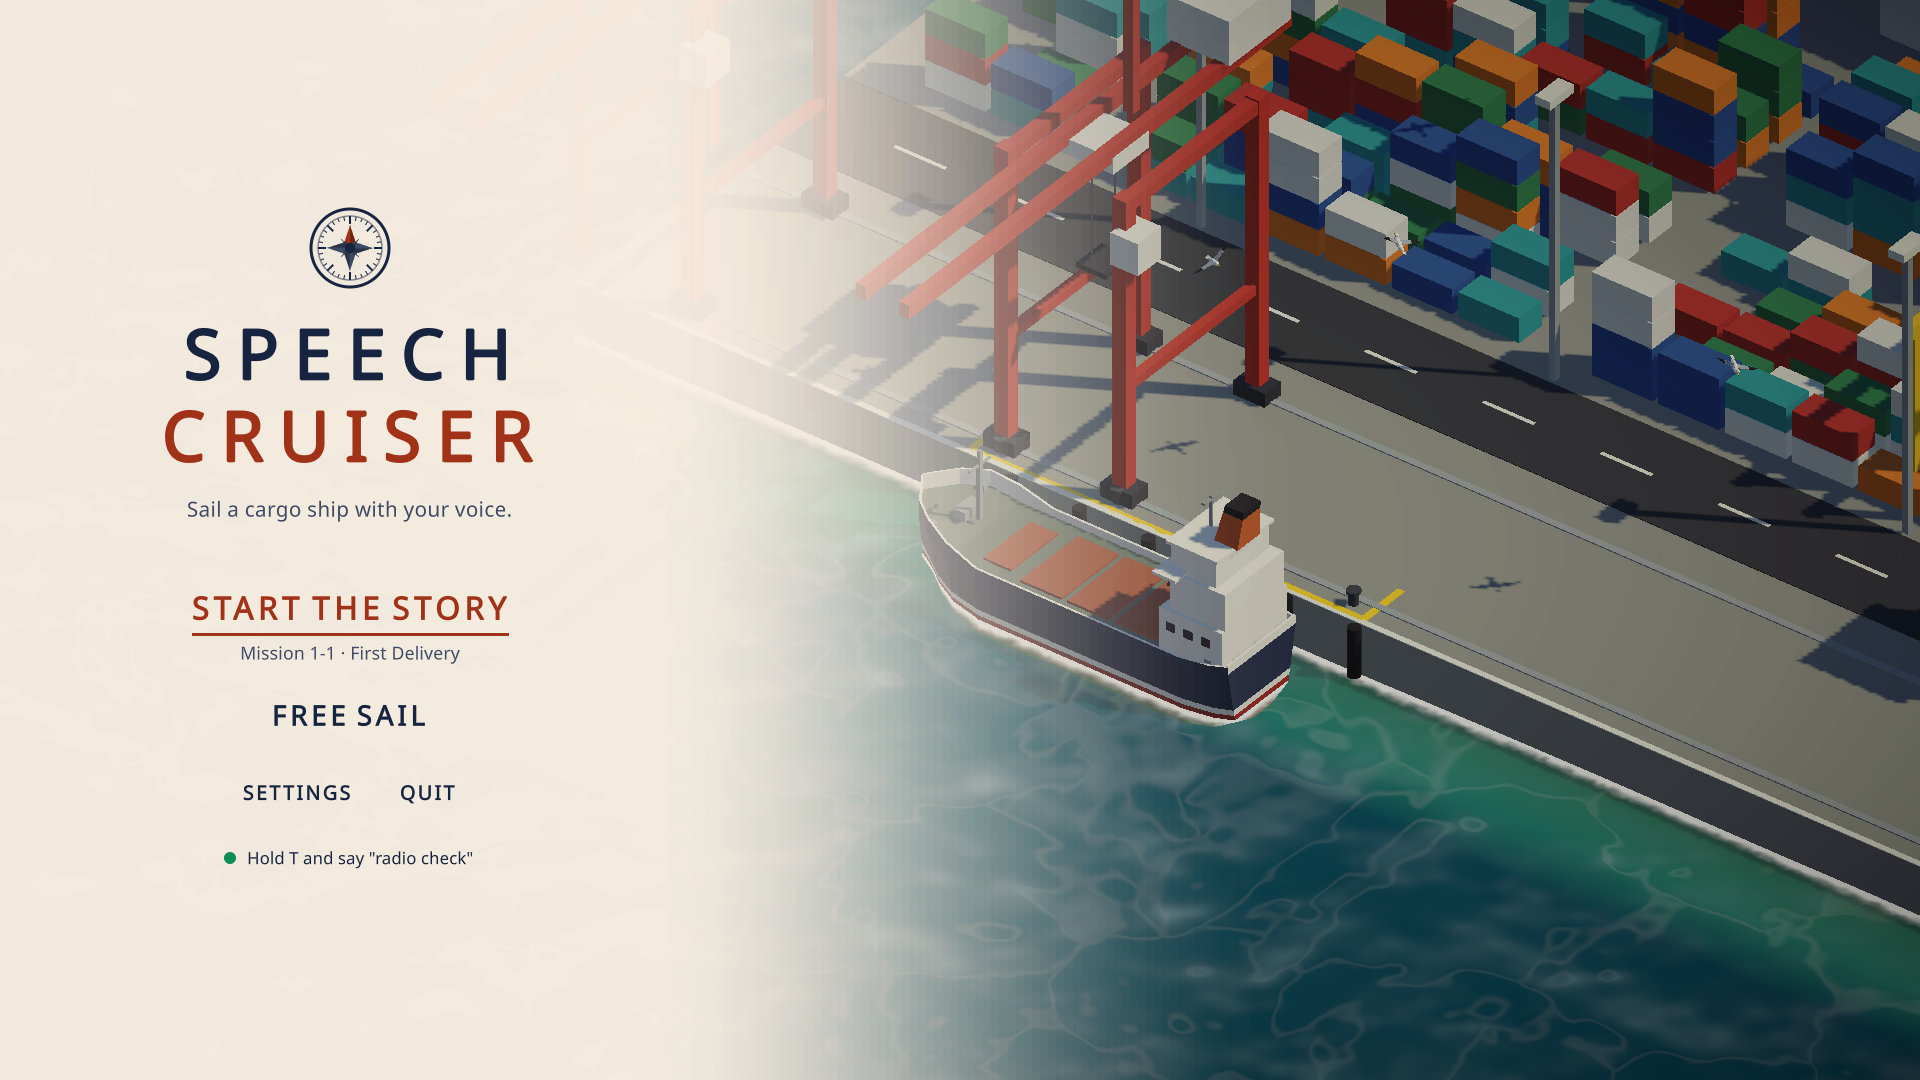
\includegraphics[width=\linewidth]{Document/GameDev/images/MainMenu.png}\vspace{0.1cm} &
\textbf{ฉากที่ 1: เมนูหลัก}\newline
เกมเริ่มที่เมนูหลัก ผู้เล่นเลือกโหมดเนื้อเรื่องหรือเดินเรืออิสระ ปุ่มโหมดเนื้อเรื่องแสดงชื่อภารกิจถัดไป และด้านล่างแสดงสถานะไมโครโฟนพร้อมชวนให้ผู้เล่นทดสอบวิทยุก่อนเริ่มเล่น \\ \hline

\vspace{0.1cm}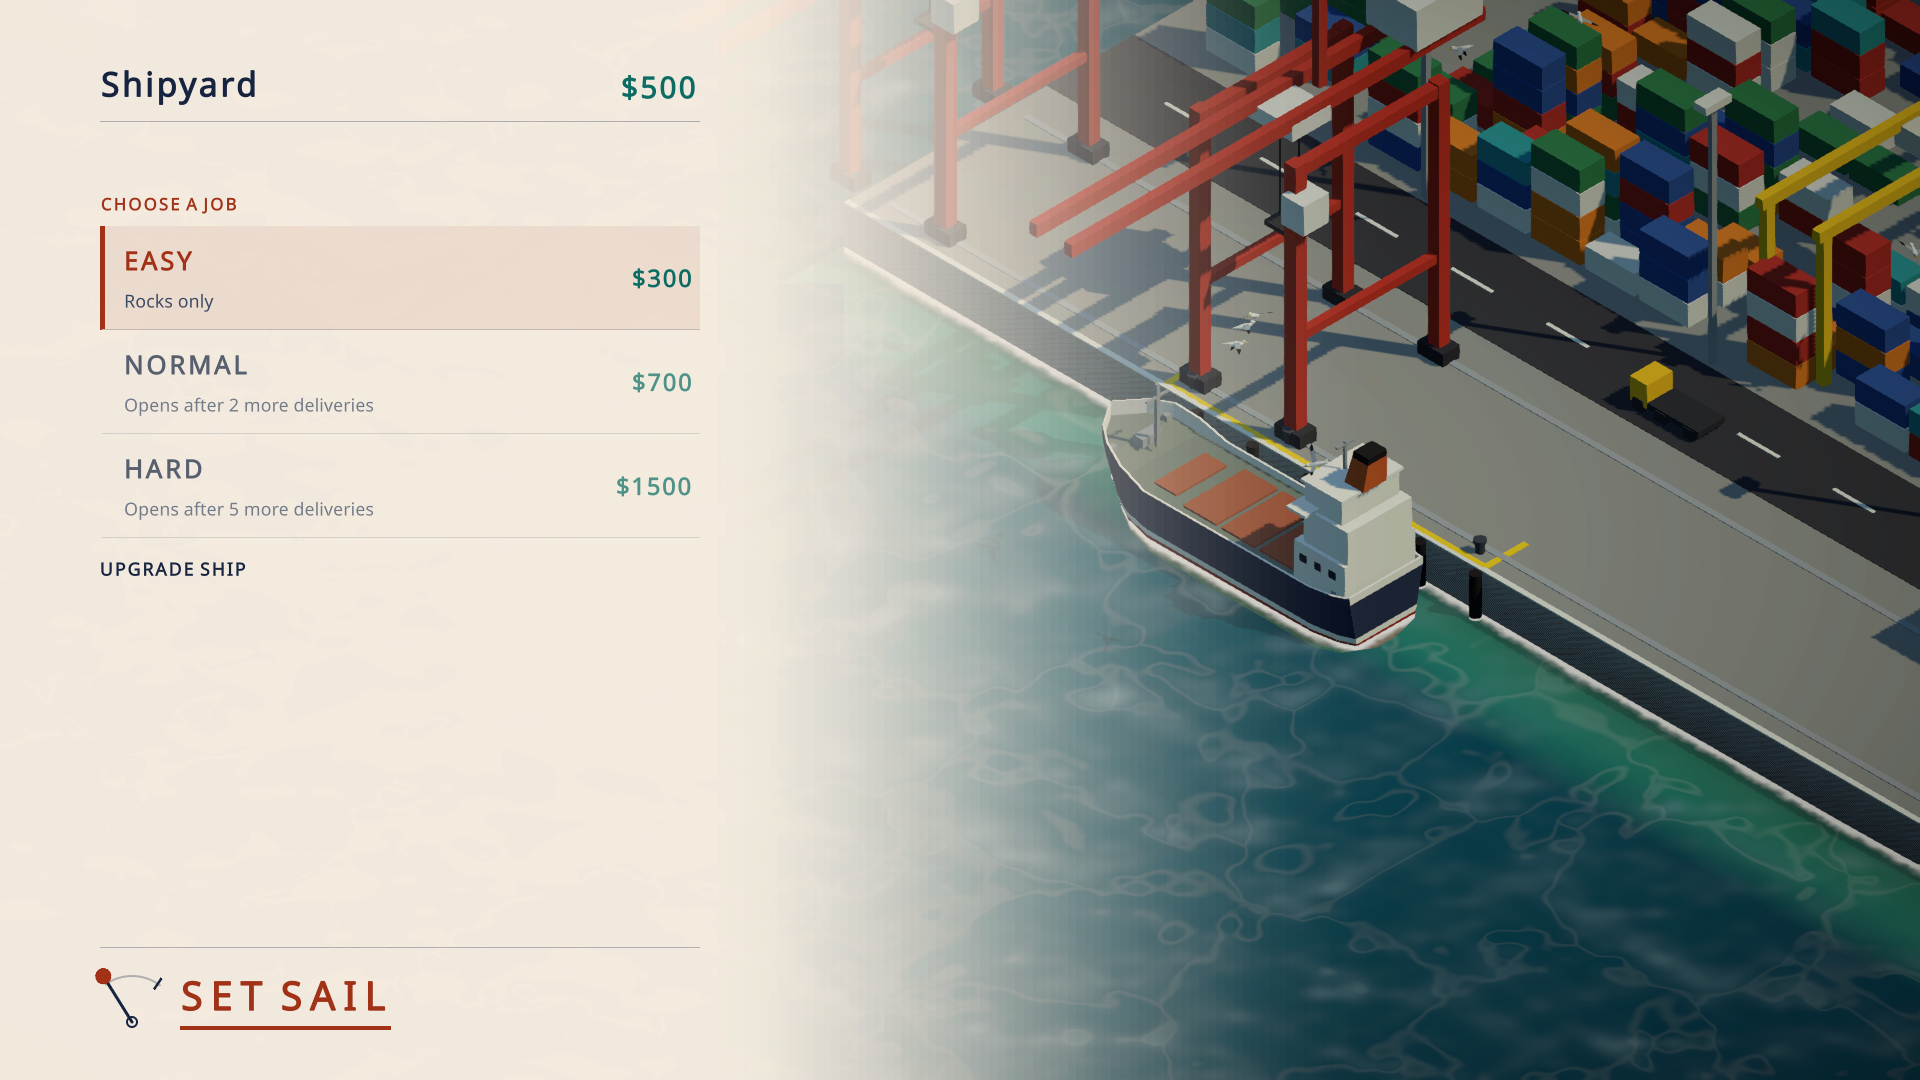
\includegraphics[width=\linewidth]{Document/GameDev/images/Shipyard.png}\vspace{0.1cm} &
\textbf{ฉากที่ 2: การรับมอบหมายภารกิจ}\newline
ในโหมดเดินเรืออิสระ ผู้เล่นเริ่มต้นในฐานะกัปตันเรือที่อู่ต่อเรือ (Shipyard) พร้อมเสียงคลื่นและนกนางนวลเพื่อสร้างความรู้สึกดื่มด่ำ (Immersion) กัปตันเลือกงานขนส่งสินค้าตามระดับความยาก แล้วสั่งออกเรือ (Set Sail) เพื่อนำเรือไปเทียบท่าปลายทางอย่างปลอดภัย ส่วนในโหมดเนื้อเรื่อง ภารกิจเริ่มจากบทสนทนาแนะนำเรื่องราวก่อนออกเรือ \\ \hline

\vspace{0.1cm}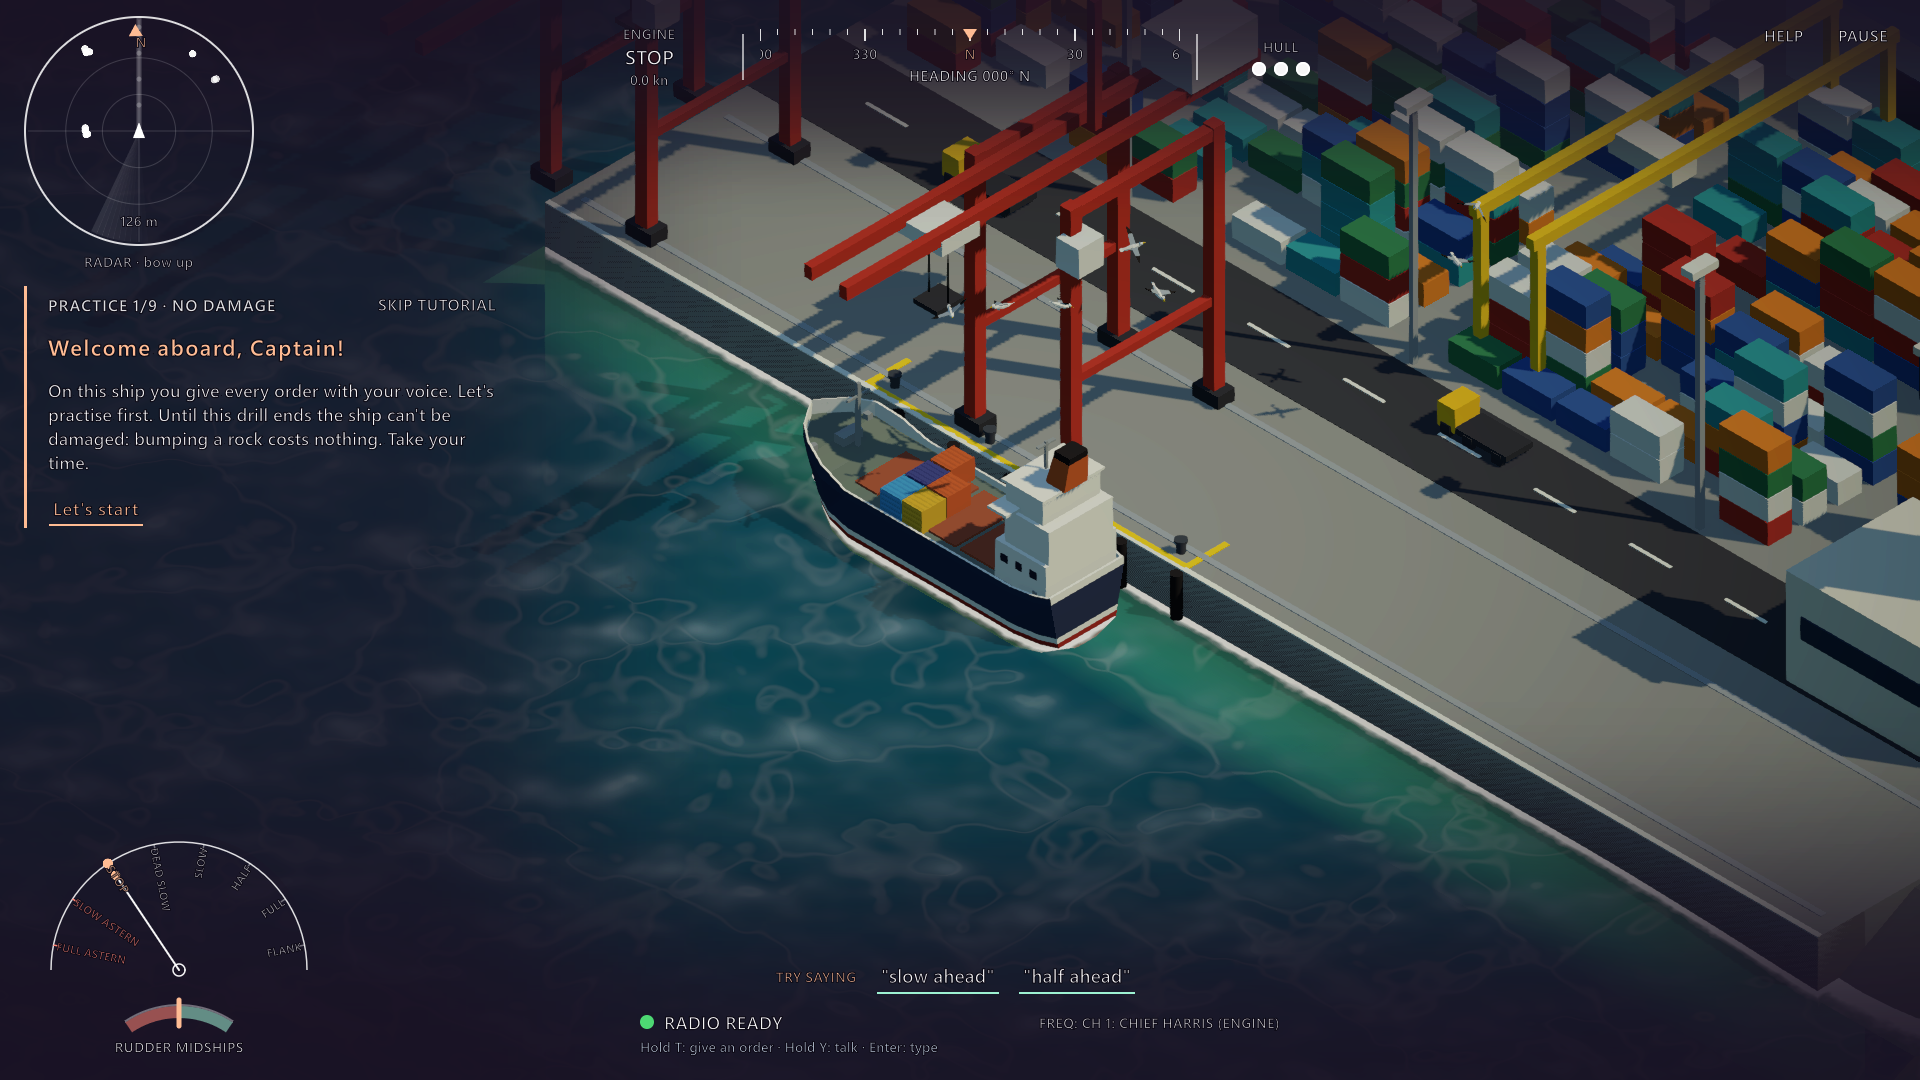
\includegraphics[width=\linewidth]{Document/GameDev/images/Tutorial.png}\vspace{0.1cm} &
\textbf{ฉากที่ 3: การแนะนำลูกเรือปัญญาประดิษฐ์}\newline
แนะนำลูกเรือทั้งสองตำแหน่ง ได้แก่ ต้นกลเรือผู้รอรับคำสั่งเครื่องยนต์และความเร็ว และพลถือท้ายผู้รอรับคำสั่งหางเสือและคอยแจ้งเตือนภัยจากเรดาร์ ในการเดินเรือครั้งแรก เกมเริ่มบทฝึกสอน (Tutorial) การออกคำสั่งเสียงภาษาอังกฤษพื้นฐาน \\ \hline
\end{tabular}
\end{table}

\begin{table}[!htbp]
\centering
\caption{ลำดับเหตุการณ์และสตอรี่บอร์ดของเกมเดินเรือ (ฉากที่ 4--6)}
\label{tab:storyboard2}
\begin{tabular}{|L{3.98cm}|L{9.74cm}|}
\hline
\textbf{ภาพประกอบ} & \textbf{คำอธิบายเนื้อเรื่องและเหตุการณ์} \\
\hline
\vspace{0.1cm}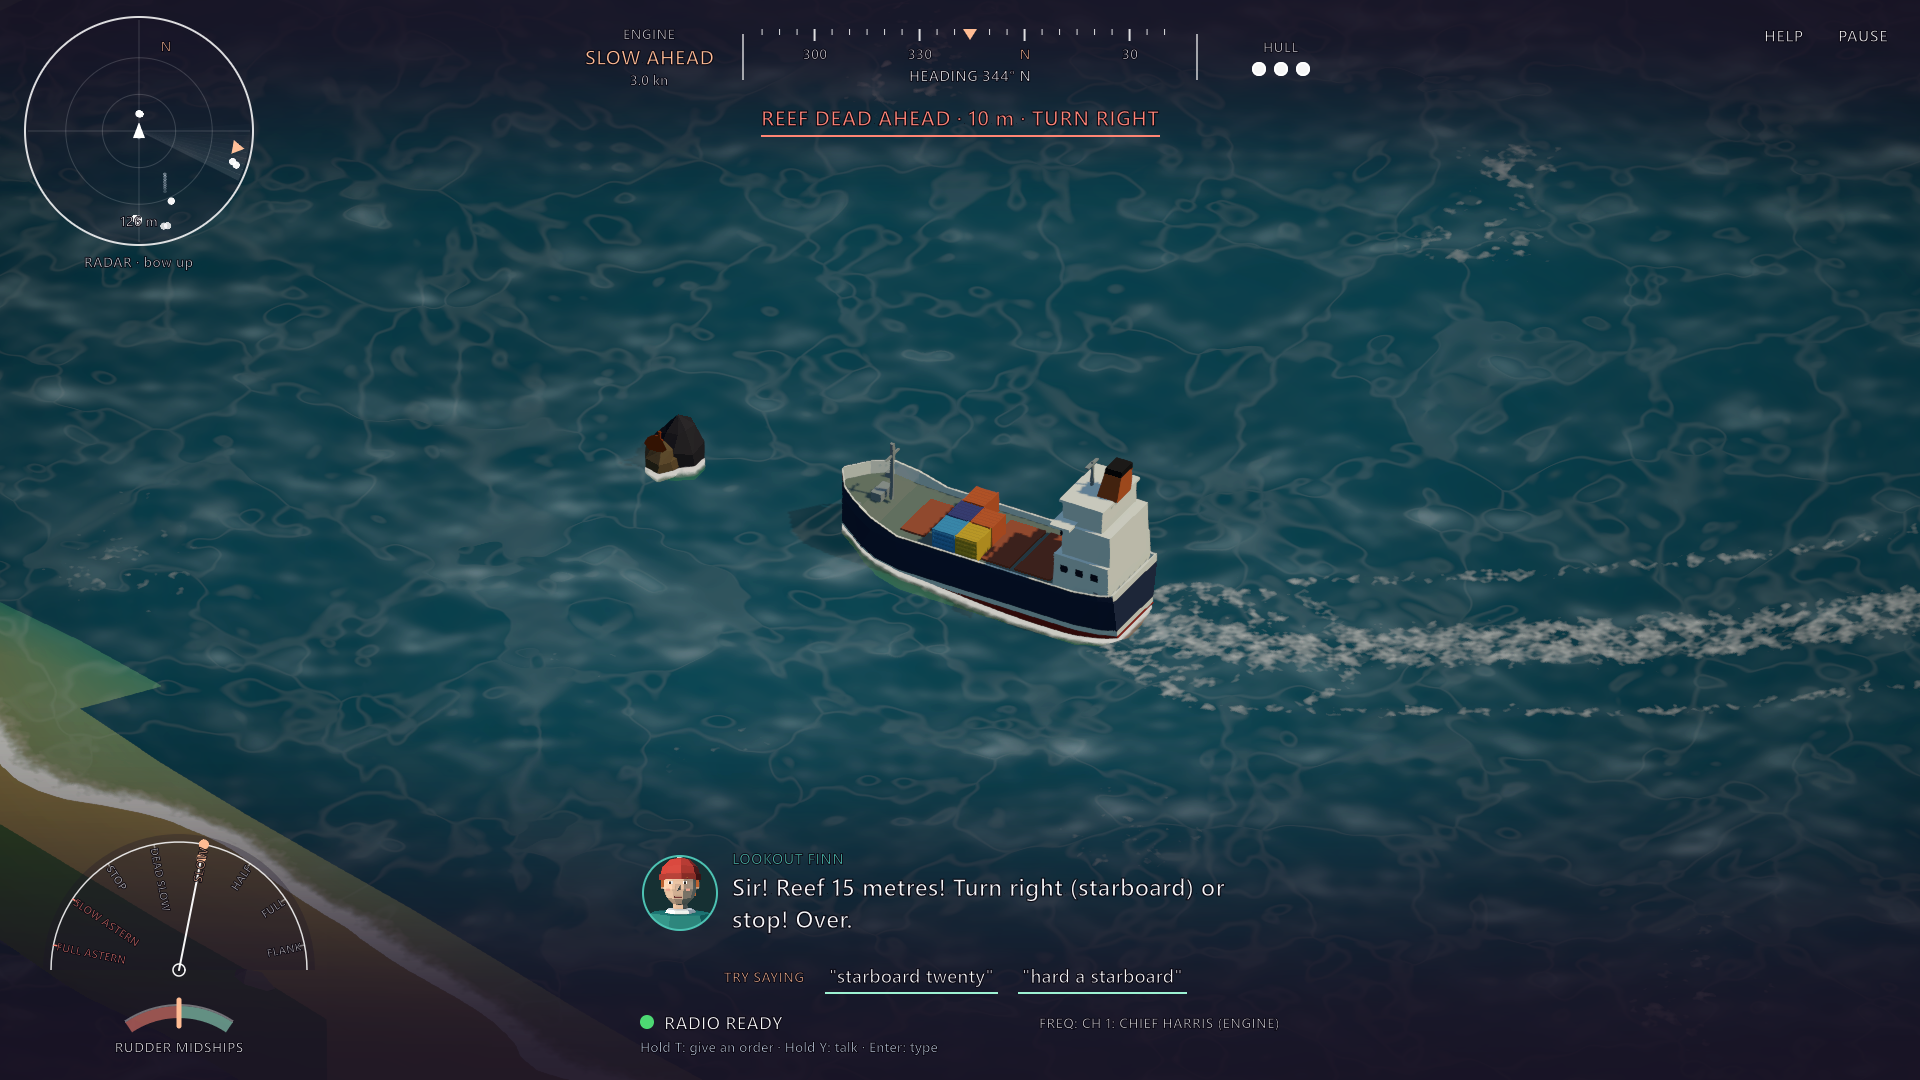
\includegraphics[width=\linewidth]{Document/GameDev/images/Hazard.png}\vspace{0.1cm} &
\textbf{ฉากที่ 4: สถานการณ์เผชิญหน้าสิ่งกีดขวาง}\newline
ระหว่างทางมีอุปสรรค เช่น แนวหินโสโครกหรือทุ่นระเบิดขวางหน้า เรดาร์และยามระวังหน้าส่งสัญญาณเตือนภัยพร้อมบอกระยะและทิศทางที่ควรหลบ ผู้เล่นต้องประเมินสถานการณ์และสั่งการให้ทันเวลา และในโหมดเนื้อเรื่อง ผู้เล่นต้องพูดคำสั่งฉุกเฉินที่แสดงบนจอภายในเวลาที่กำหนด \\ \hline

\vspace{0.1cm}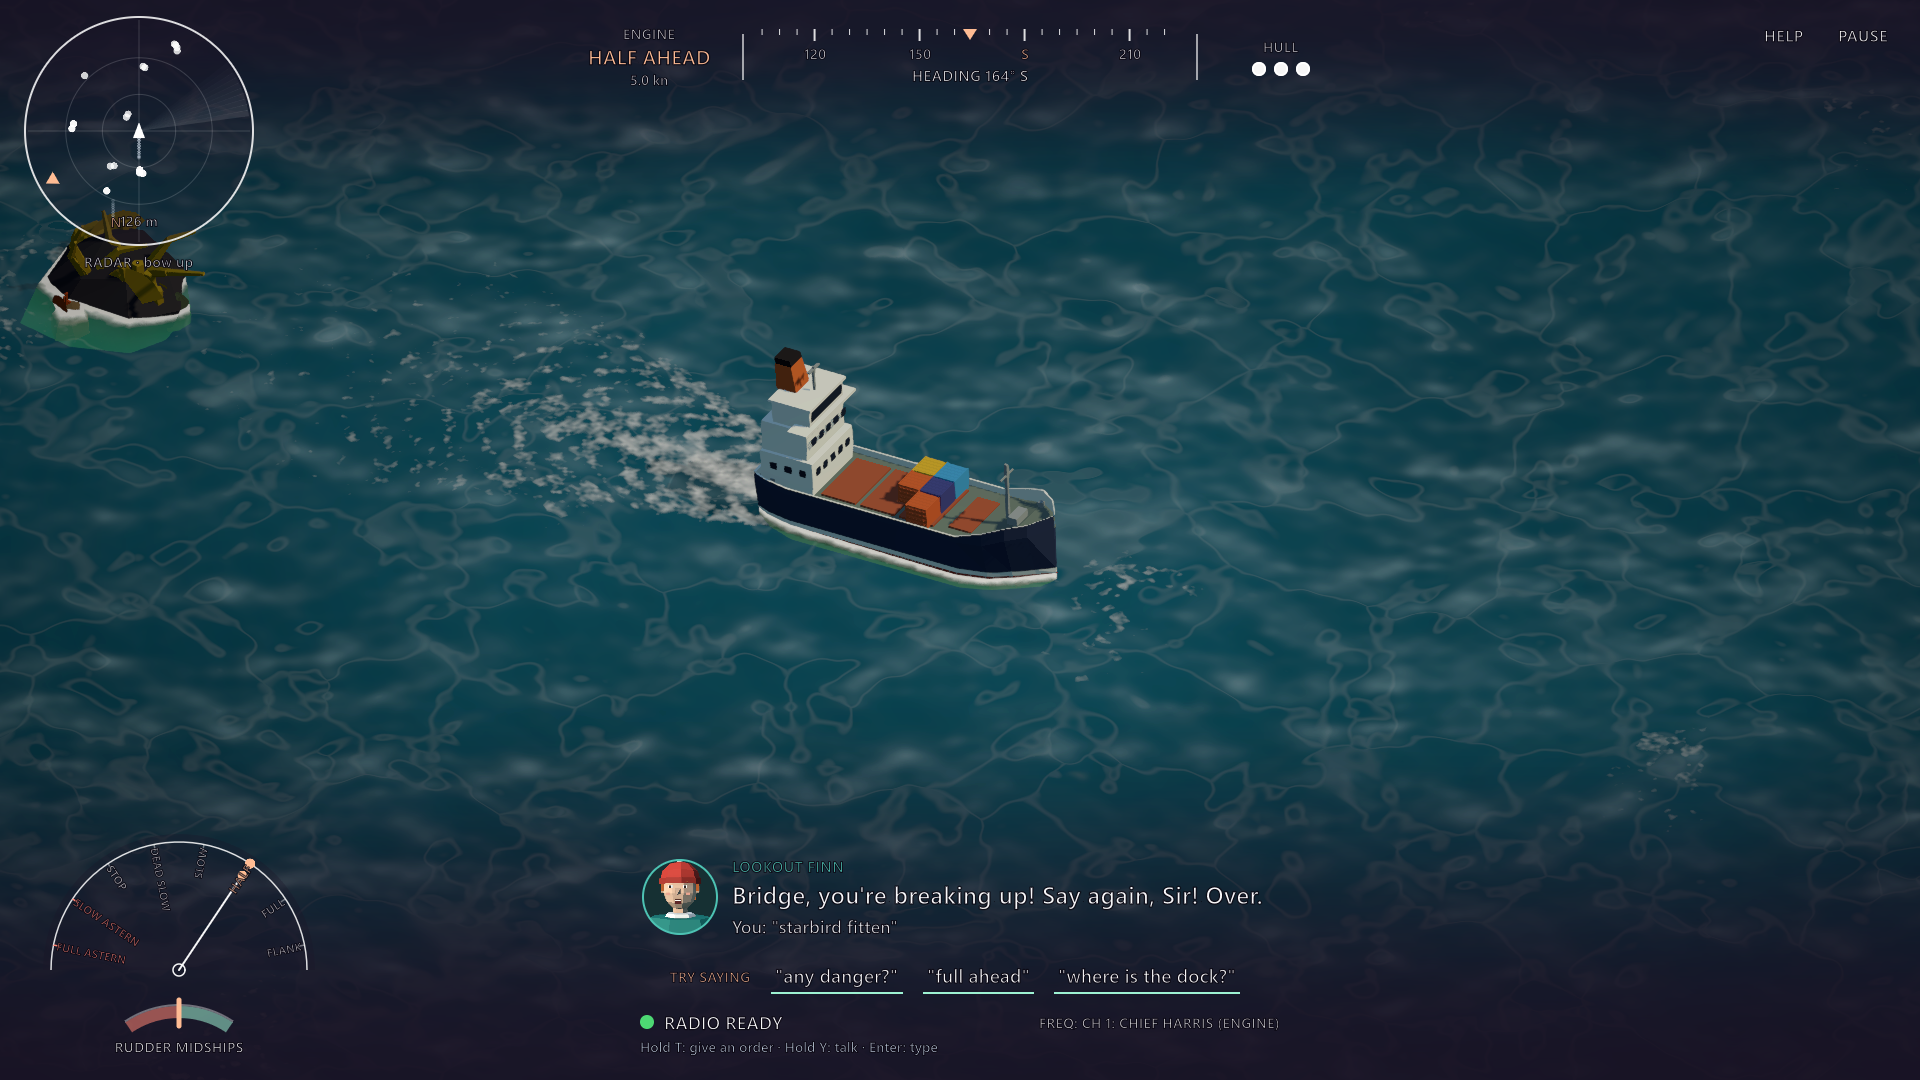
\includegraphics[width=\linewidth]{Document/GameDev/images/Sayagain.png}\vspace{0.1cm} &
\textbf{ฉากที่ 5: สถานการณ์สื่อสารติดขัด (Clarification Request)}\newline
หากผู้เล่นออกเสียงไม่ชัดเจนหรือใช้คำสั่งที่ระบบไม่เข้าใจ ลูกเรือจะขอให้พูดซ้ำ (Say again) เช่น \textit{``Say again, Bridge. Over.''} และให้คำใบ้รูปประโยคมาตรฐานเมื่อไม่เข้าใจติดกัน 2 ครั้ง เพื่อกระตุ้นให้ผู้เล่นแก้ไขการสื่อสารและเปล่งเสียงให้ชัดเจนขึ้น \\ \hline

\vspace{0.1cm}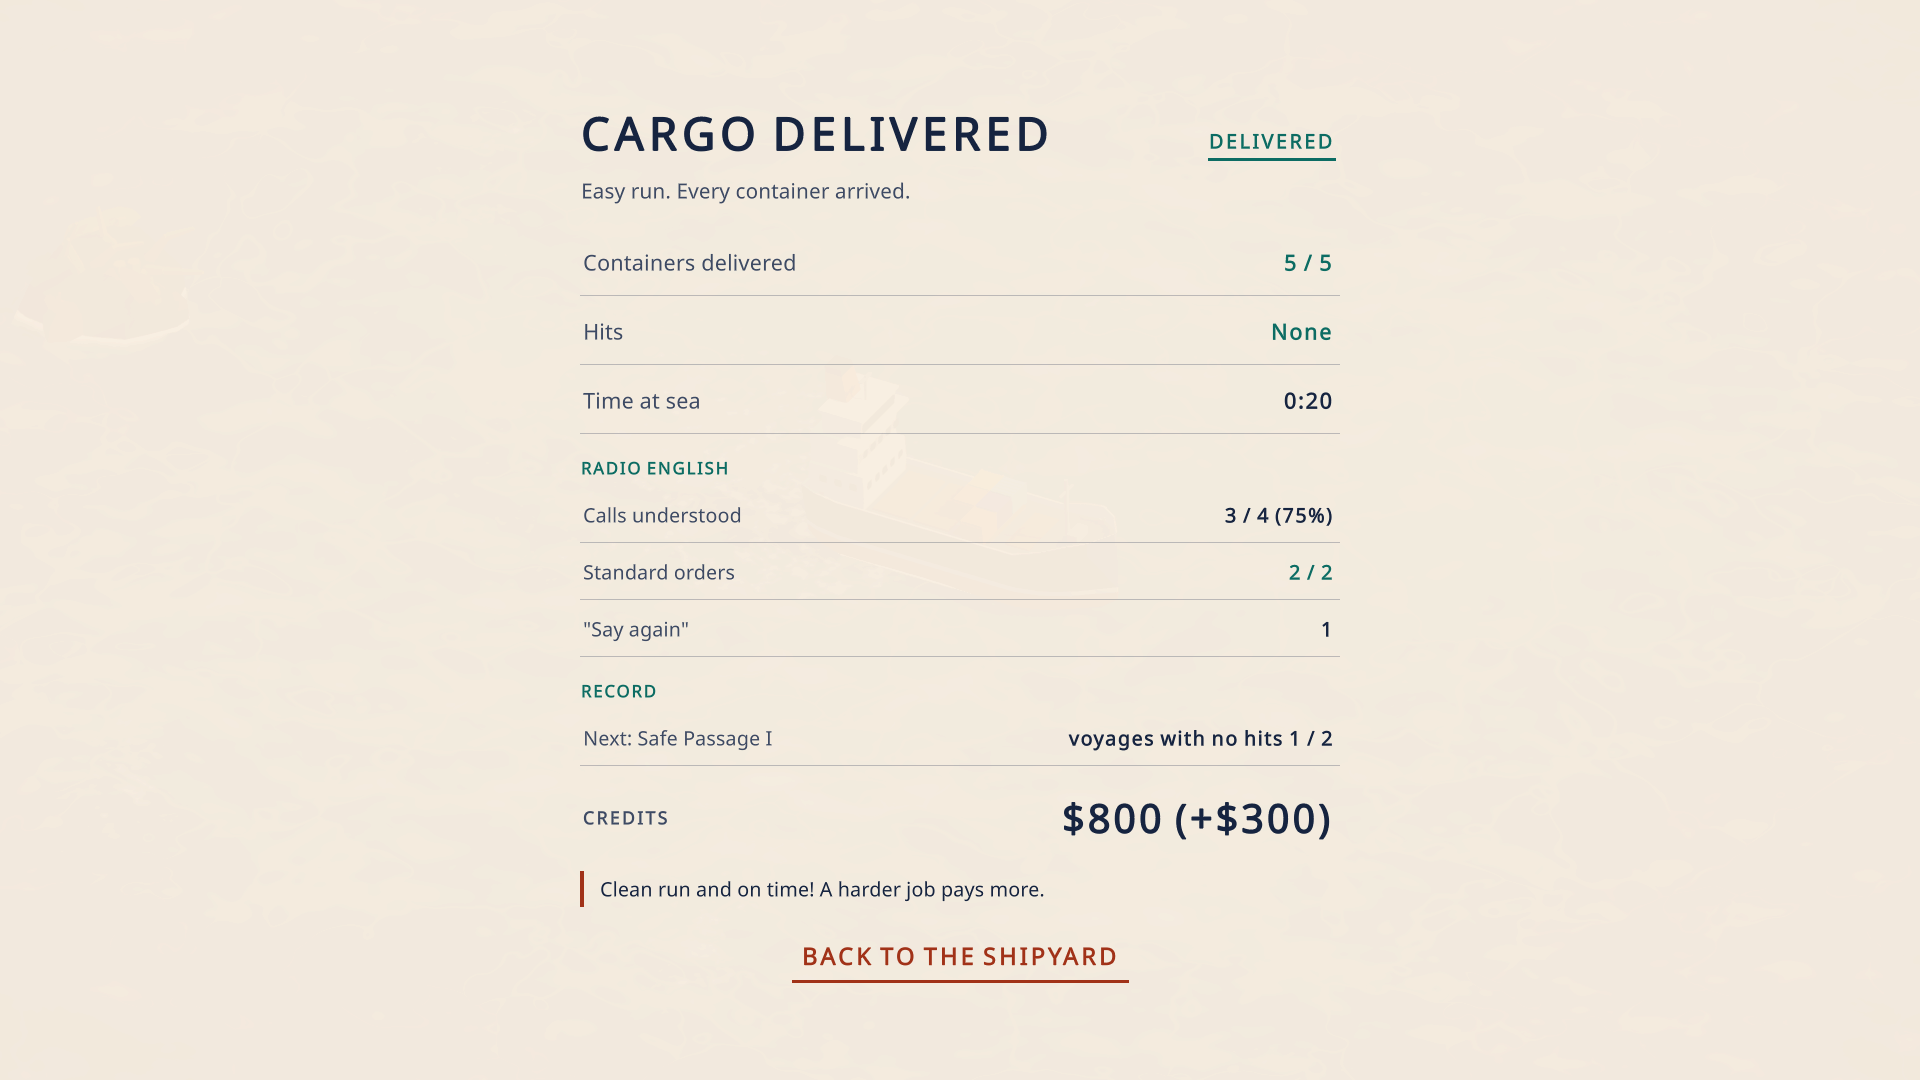
\includegraphics[width=\linewidth]{Document/GameDev/images/Victory.png}\vspace{0.1cm} &
\textbf{ฉากที่ 6: สรุปผลภารกิจ (Result Screen)}\newline
หากนำเรือเทียบท่าและผูกเรือได้สำเร็จ เกมจะแสดงหน้าจอสรุปผล (Cargo Delivered) พร้อมสรุปการสื่อสารภาษาอังกฤษทางวิทยุ ได้แก่ สัดส่วนคำสั่งที่ลูกเรือเข้าใจ จำนวนคำสั่งมาตรฐาน และจำนวนครั้งที่ลูกเรือขอให้พูดซ้ำ แต่หากชนสิ่งกีดขวางจนความทนทานของตัวเรือ (Hull) ลดลงเหลือศูนย์ จะแสดงหน้าจอเรืออับปาง (Ship Lost) และเรือลากจูงจะลากเรือกลับท่าโดยผู้เล่นเสียค่าลากเรือ \\
\hline
\end{tabular}
\end{table}

% -----------------------------------------------------------
% 4.3 การออกแบบระบบการเล่น
% -----------------------------------------------------------
\section{การออกแบบระบบการเล่น}

\subsection{วิธีการเล่นเกม (How to Play)}

ผู้เล่นรับบทเป็นกัปตันเรือขนส่งสินค้า มีหน้าที่สั่งการลูกเรือเพื่อนำเรือไปเทียบท่าปลายทางอย่างปลอดภัย กติกาการเล่นหลักมีดังนี้

\begin{enumerate}[label=\arabic*)]
    \item \textbf{การควบคุมผ่านวิทยุ:} ผู้เล่นไม่มีปุ่มบังคับหางเสือหรือเครื่องยนต์โดยตรง แต่ต้องออกคำสั่งเป็นภาษาอังกฤษทางวิทยุถึงลูกเรือปัญญาประดิษฐ์ ด้วยเสียง (ปุ่ม T) หรือพิมพ์คำสั่ง (ปุ่ม Enter) ขั้นตอนการสั่งการโดยละเอียดแสดงในตารางที่ \ref{tab:uc_order}
    \item \textbf{การหลบหลีกสิ่งกีดขวาง:} ร่องน้ำมีชายฝั่งและแนวหินกั้นทั้งสองข้าง และมีหิน แนวหินโสโครก สันดอน และทุ่นระเบิดกระจายอยู่ภายในร่องน้ำ ทุ่นระเบิดมีตั้งแต่ระดับ Normal ขึ้นไป และการชนทุ่นระเบิดทำให้เสียตู้สินค้า 2 ตู้ ส่วนสันดอนทำให้เรือเกยตื้นโดยไม่เสียหาย และผู้เล่นต้องสั่งถอยเรือออก ผู้เล่นต้องประเมินสถานการณ์จากภาพมุมไอโซเมตริกและเรดาร์ แล้วออกคำสั่งให้ทันเวลา เช่น ``Starboard fifteen'' หรือ ``Stop engine''
    \item \textbf{การตอบสนองของลูกเรือ:} หากลูกเรือเข้าใจคำสั่ง ลูกเรือที่รับผิดชอบจะทวนคำสั่งและบังคับเรือ ซึ่งเคลื่อนที่ตามแบบจำลองที่มีแรงเฉื่อย หากไม่เข้าใจ ลูกเรือจะตอบกลับตามบริบทหรือขอให้พูดซ้ำ (Say again)
    \item \textbf{ผลลัพธ์ของภารกิจ:}
    \begin{itemize}[leftmargin=1.5em,labelindent=0pt]
        \item \textbf{สำเร็จ (Cargo Delivered):} นำเรือถึงท่าปลายทาง ขอเทียบท่า (Request Docking) และผูกเรือ (Make Fast) ได้ก่อนความทนทานของตัวเรือหมด โดยการชนแต่ละครั้งทำให้ตู้สินค้าตกน้ำและค่าตอบแทนลดลง
        \item \textbf{ล้มเหลว (Ship Lost):} ชนสิ่งกีดขวางจนความทนทานของตัวเรือเหลือศูนย์ เรือลากจูงจะลากเรือกลับท่าโดยผู้เล่นเสียค่าลากเรือ
    \end{itemize}
\end{enumerate}

\subsection{กระบวนการเล่นหลัก (Core Game Loop)}

กระบวนการเล่นหลักแสดงกิจกรรมที่ผู้เล่นทำซ้ำระหว่างการเดินเรือหนึ่งรอบ และการโต้ตอบระหว่างผู้เล่น ลูกเรือ และแบบจำลองการเคลื่อนที่ของเรือ ดังภาพที่ \ref{fig:gameloop} ส่วนการเปลี่ยนสถานะของระบบทั้งเกม ตั้งแต่เมนูหลักจนถึงหน้าสรุปผล แสดงแยกเป็นแผนภาพสถานะในภาพที่ \ref{fig:state_main} ในภาคผนวก ค

\MermaidAdjustBoxOpts{max width=\linewidth, max height=0.88\textheight, center}
\begin{figure}[!htbp]
\centering
\begin{mermaid}
%%{init: {'flowchart': {'nodeSpacing': 25, 'rankSpacing': 28}}}%%
graph TD
    A[เริ่มภารกิจ] --> B[ประเมินสถานการณ์จากเรดาร์และภาพทะเล]
    B --> E[ผู้เล่นออกคำสั่ง เสียงหรือพิมพ์]
    E --> F[แปลงเสียงเป็นข้อความ]
    F --> G{ตัวแยกคำสั่งพบคำสั่งหรือไม่}
    G -- ไม่พบ --> Q[GPT-4o mini จำแนกเจตนา]
    Q --> R{พบคำสั่งหรือไม่}
    R -- ไม่พบ --> H[ลูกเรือสนทนาตอบ หรือขอให้พูดซ้ำ]
    H --> B
    R -- พบ --> I[ลูกเรือทวนคำสั่ง]
    G -- พบ --> I
    I --> J[เรือเคลื่อนที่ตามคำสั่ง]
    J --> K{ชนสิ่งกีดขวางหรือไม่}
    K -- ชน --> N[ความทนทานของตัวเรือลดลง ตู้สินค้าตกน้ำ]
    N --> O{ความทนทานเหลือ 0 หรือไม่}
    O -- เหลือ 0 --> P[Ship Lost ลากเรือกลับท่า]
    O -- ยังไม่เหลือ 0 --> B
    K -- ไม่ชน --> L{ถึงท่าปลายทางหรือยัง}
    L -- ยังไม่ถึง --> B
    L -- ถึงแล้ว --> S[ขอเทียบท่าและผูกเรือ]
    S --> M[Cargo Delivered]
\end{mermaid}
\caption{แผนภาพกระบวนการเล่นหลัก (Core Game Loop)}
\label{fig:gameloop}
\end{figure}
\MermaidAdjustBoxOpts{max width=\linewidth, max height=0.65\textheight, center}

จากภาพที่ \ref{fig:gameloop} ผู้เล่นออกคำสั่งได้ตลอดการเดินเรือ ไม่เฉพาะเมื่อพบสิ่งกีดขวาง ความท้าทายหลักของเกมไม่ได้อยู่ที่การกดปุ่ม แต่อยู่ที่การบริหารเวลาในการพูดคำสั่งและการแก้ปัญหาการสื่อสาร ขณะที่เรือยังคงเคลื่อนที่ต่อเนื่อง

\subsection{สถาปัตยกรรมของระบบ (System Architecture)}

สถาปัตยกรรมระบบเกมเดินเรือด้วยระบบสั่งการด้วยเสียงแสดงดังภาพที่ \ref{fig:architecture}

\begin{figure}[!htbp]
\centering
\begin{mermaid}
graph TD
    subgraph Client["Player PC (Client)"]
        Unity["Unity Engine (Game Client)"]
        Mic["Microphone (Audio Input)"]
        Speaker["Speaker/Headphones (Audio Output)"]
    end

    subgraph Core["Core Systems"]
        GameLogic["C# Game Logic, Command Parser and Ship Physics"]
        UI["UI and HUD"]
        STT["Speech-to-Text (Whisper, whisper.cpp on-device)"]
        TTS["Windows Speech (TTS)"]
    end

    subgraph ExternalAPI["External API"]
        LLM["OpenAI API (GPT-4o mini)"]
    end

    Mic -->|Voice Input| Unity
    Unity -->|Audio Clip| STT
    STT -->|Text| GameLogic
    GameLogic -->|unclear text / chat only| LLM
    LLM -->|intent JSON / reply text| GameLogic
    GameLogic -->|Control| UI
    GameLogic -->|crew line text| TTS
    TTS -->|crew voice| Speaker
\end{mermaid}
\caption{สถาปัตยกรรมของระบบเกม}
\label{fig:architecture}
\end{figure}

จากภาพที่ \ref{fig:architecture} ระบบทำงานบนเกมเอนจิน Unity เป็นหลัก โดยรับเสียงพูดภาษาอังกฤษผ่านไมโครโฟน และแปลงเป็นข้อความด้วยโมเดลการรู้จำเสียง Whisper~\cite{radford2023} ซึ่งทำงานภายในเครื่องของผู้เล่นผ่านไลบรารี whisper.cpp โดยไม่ส่งเสียงออกไปยังเครือข่าย จากนั้นตัวแยกคำสั่งภายในเครื่องแปลข้อความเป็นคำสั่งควบคุมเรือ ระบบส่งข้อความไปยัง GPT-4o mini ผ่านเครือข่ายเฉพาะ 2 กรณี ได้แก่ คำสั่งที่ตัวแยกคำสั่งไม่เข้าใจ (เพื่อจำแนกเจตนาเป็น JSON) และการสนทนากับลูกเรือ (เพื่อสร้างข้อความตอบกลับ) GPT-4o mini ส่งกลับมาเพียงข้อความ ส่วนเสียงของลูกเรือสร้างด้วยระบบสังเคราะห์เสียงของ Windows (Windows Speech) บนเครื่องของผู้เล่น

\subsection{แผนภาพการติดตั้ง (Deployment Diagram)}

แผนภาพการติดตั้งแสดงการจัดวางส่วนประกอบของเกมบนเครื่องของผู้เล่น ดังภาพที่ \ref{fig:deployment} เกมทั้งหมดรวมถึงโมเดลการรู้จำเสียงติดตั้งอยู่ในเครื่องคอมพิวเตอร์ของผู้เล่น มีเพียงบริการ OpenAI ที่เรียกผ่านอินเทอร์เน็ต

\begin{figure}[!htbp]
\centering
\begin{mermaid}
graph TD
    subgraph PC["เครื่องคอมพิวเตอร์ของผู้เล่น (Windows 10/11)"]
        Mic["ไมโครโฟน / ชุดหูฟัง"]
        subgraph App["SpeechCruiser.exe (Unity)"]
            Game["ตรรกะเกม ฟิสิกส์เรือ และ UI"]
            Whisper["whisper.cpp + ggml-base.en.bin"]
            TTS["เสียงลูกเรือ (Windows Speech)"]
        end
        Prefs["PlayerPrefs (Registry)"]
        Logs["แฟ้ม CSV ในโฟลเดอร์ Sessions"]
        Key["OPENAI_API_KEY หรือ openai.key"]
    end

    subgraph Cloud["บริการภายนอก"]
        OpenAI["OpenAI API (GPT-4o mini)"]
    end

    Mic -- "เสียงพูด" --> Whisper
    Whisper -- "ข้อความ" --> Game
    Game --> TTS
    Game --> Prefs
    Game --> Logs
    Key -.-> Game
    Game -- "HTTPS :443 (เฉพาะเมื่อจำเป็น)" --> OpenAI
\end{mermaid}
\caption{แผนภาพการติดตั้งระบบ}
\label{fig:deployment}
\end{figure}

จากภาพที่ \ref{fig:deployment} ระบบไม่ส่งเสียงของผู้เล่นออกนอกเครื่อง ข้อมูลที่ส่งไปยังบริการ OpenAI มีเพียงข้อความที่ถอดได้และสถานะของเรือ

\subsection{โครงสร้างโฟลเดอร์ของโครงการ (Project Structure)}

โครงสร้างแฟ้มข้อมูลของโครงการที่พัฒนาด้วยเกมเอนจิน Unity แสดงดังตารางที่ \ref{tab:folder}

\begin{table}[!htbp]
\centering
\caption{โครงสร้างโฟลเดอร์หลักของโครงการ}
\label{tab:folder}
\begin{tabular}{|L{4.50cm}|L{9.20cm}|}
\hline
\textbf{โฟลเดอร์} & \textbf{คำอธิบาย} \\
\hline
\texttt{Assets/Scenes/} & ฉาก Menu (เมนูหลักและโหมดเนื้อเรื่อง) และฉาก Game (อู่ต่อเรือ การเดินเรือ และหน้าสรุปผล) \\ \hline
\texttt{Assets/Script/} & ชุดคำสั่งภาษา C\# สำหรับแบบจำลองการเคลื่อนที่ของเรือ การรับคำสั่งเสียง ลูกเรือ และระบบ UI โดยมีโฟลเดอร์ย่อย เช่น \texttt{Command/} (ตัวแยกคำสั่ง) \texttt{Ship/} (สร้างโมเดลเรือของผู้เล่นด้วยโค้ด) \texttt{Teaching/} (ระบบช่วยสอนภาษาและบันทึกผลการทดลอง) และ \texttt{Story/} (โหมดเนื้อเรื่อง) \\ \hline
\texttt{Assets/Script/LLMManager/} & ชุดคำสั่งสำหรับเชื่อมต่อ OpenAI API \\ \hline
\texttt{Assets/Whisper/} & แพ็กเกจ whisper.unity (ไลบรารี whisper.cpp) สำหรับรู้จำเสียงภายในเครื่อง โดยแฟ้มโมเดล ggml-base.en เก็บอยู่ที่ \texttt{Assets/StreamingAssets/Whisper/} \\ \hline
\texttt{Assets/Prefab/} & วัตถุสำเร็จรูป ได้แก่ ตู้สินค้า ทุ่นระเบิด แนวหิน และท่าเรือ \\ \hline
\texttt{Assets/Mesh/} & แฟ้มโมเดล 3 มิติ (3D Models) ของตู้สินค้า ทุ่นระเบิด แนวหิน และท่าเรือ \\ \hline
\texttt{Assets/Audio/} & ดนตรีประกอบและเสียงเอฟเฟกต์ (SFX) ส่วนเสียงทะเลและนกนางนวลสังเคราะห์ด้วยโค้ด \\ \hline
\texttt{Assets/UI/} & แฟ้มโครงหน้าจอ (UXML) และรูปแบบการแสดงผล (USS) ของ UI Toolkit สำหรับเมนู HUD และอู่ต่อเรือ \\
\hline
\end{tabular}
\end{table}

\subsection{การออกแบบหน้าจอ}

ผู้จัดทำออกแบบหน้าจอของเกมให้จำลองสถานการณ์การเดินเรือได้สมจริงและอ่านข้อมูลง่าย โดยไม่บดบังภาพทะเล หน้าจอหลักของเกมแสดงดังตารางที่ \ref{tab:mockups}

\begin{table}[!htbp]
\centering
\caption{รายการต้นแบบหน้าจอ}
\label{tab:mockups}
\begin{tabular}{|L{1.48cm}|L{3.44cm}|L{8.36cm}|}
\hline
\textbf{รหัสหน้าจอ} & \textbf{ชื่อหน้าจอ} & \textbf{ส่วนประกอบหลัก} \\
\hline
UI-01 & หน้าจอหลัก (Main Menu) & ชื่อเกม ปุ่มโหมดเนื้อเรื่อง (Story) ที่บอกภารกิจถัดไป ปุ่มเดินเรืออิสระ (Free Sail) ปุ่มเริ่มอาชีพใหม่ (New Career) ปุ่มตั้งค่า (Settings) ปุ่มออกเกม (Quit) และสถานะไมโครโฟนพร้อมคำแนะนำให้ทดสอบวิทยุ \\ \hline
UI-02 & หน้าจอเล่นเกม (Gameplay HUD) & ภาพเรือมุมไอโซเมตริก เรดาร์ เข็มทิศและองศาหัวเรือ คันโทรเลขเครื่องยนต์และความเร็ว ตัวแสดงมุมหางเสือ ความทนทานของตัวเรือ (Hull) กล่องสถานะวิทยุ ช่องวิทยุที่เลือก คำบรรยายบทพูดของลูกเรือ และคำแนะนำประโยคที่ควรพูด (Try Saying) \\ \hline
UI-03 & หน้าจออู่ต่อเรือ (Shipyard) & ยอดเงิน รายการงานขนส่งสินค้าตามระดับความยาก (Easy Normal Hard) พร้อมค่าตอบแทน ปุ่มอัปเกรดเรือ (Upgrade Ship) ซึ่งใช้เงินร่วมกับใบรับรองทักษะภาษา และปุ่มออกเรือ (Set Sail) โดยการซ่อมแซมเรือไม่มีค่าใช้จ่าย \\ \hline
UI-04 & หน้าจอสรุปผล (Result Screen) & หัวข้อ Cargo Delivered (Mission Complete ในโหมดเนื้อเรื่อง) หรือ Ship Lost ผลการเดินเรือ (ตู้สินค้าที่ส่งถึง หรือตู้สินค้าที่เสียและค่าลากเรือ จำนวนครั้งที่ชน เวลาที่ใช้) สรุปการสื่อสารทางวิทยุ (สัดส่วนคำสั่งที่ลูกเรือเข้าใจ จำนวนคำสั่งมาตรฐาน จำนวนครั้งที่ลูกเรือขอให้พูดซ้ำ เวลาเฉลี่ยในการสั่งหลังได้รับคำเตือน และจำนวนคำสั่งฉุกเฉินที่ทันเวลา) ความคืบหน้าของใบรับรอง เงินที่ได้รับ และคำแนะนำสำหรับรอบถัดไป \\ \hline
UI-05 & เมนูหยุดเกม (Pause) & ปุ่มเล่นต่อ (Resume) ตั้งค่า (Settings) เล่นบทฝึกสอนซ้ำ (Replay Tutorial) กลับเมนูหลัก (Main Menu) และออกเกม (Quit) \\ \hline
UI-06 & หน้าจอตั้งค่า (Settings) & เลือกไมโครโฟน ระดับเสียง ขนาดคำบรรยาย ปุ่มสั่งการและปุ่มสนทนา โหมดกดค้างหรือกดสลับเพื่อพูด และรหัสผู้เข้าร่วม (Participant Code) \\
\hline
\end{tabular}
\end{table}

\subsubsection{UI-01: หน้าจอหลัก (Main Menu)}

หน้าจอหลักเป็นหน้าแรกเมื่อเปิดเกม ใช้พื้นหลังสีกระดาษและภาพท่าเรือจริงจากในเกม ดังภาพที่ \ref{fig:ui_menu}

\begin{figure}[!htbp]
\centering
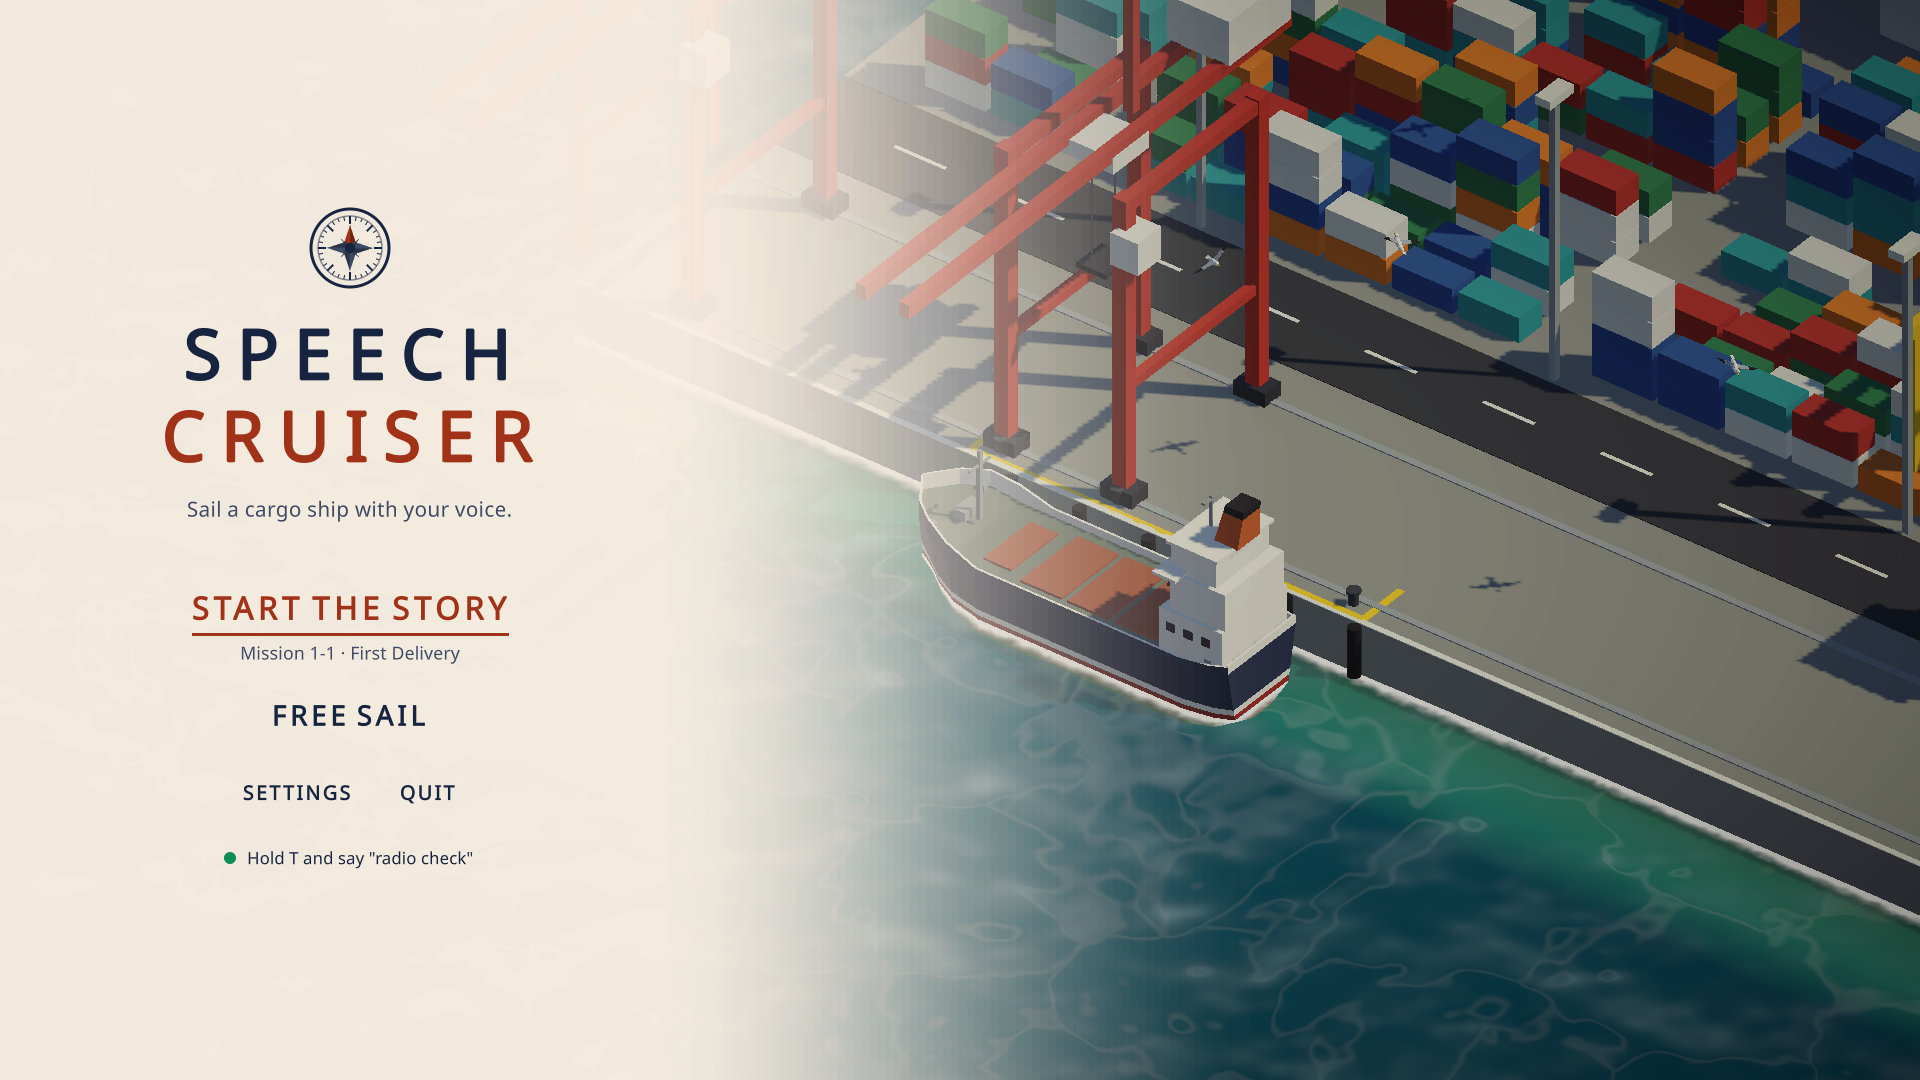
\includegraphics[width=0.8\textwidth]{Document/GameDev/images/MainMenu.png}
\caption{หน้าจอหลัก (UI-01)}
\label{fig:ui_menu}
\end{figure}

จากภาพที่ \ref{fig:ui_menu} ปุ่มโหมดเนื้อเรื่องแสดงชื่อภารกิจถัดไป (เช่น Mission 1-1 · First Delivery) ปุ่มเดินเรืออิสระพาไปยังอู่ต่อเรือ และด้านล่างแสดงสถานะไมโครโฟนพร้อมชวนให้ผู้เล่นทดสอบวิทยุด้วยคำว่า ``radio check'' ก่อนเริ่มเล่น

\subsubsection{UI-02: หน้าจอเล่นเกม (Gameplay HUD)}

หน้าจอเล่นเกมเป็นหน้าจอที่ผู้เล่นใช้ตลอดการเดินเรือ ออกแบบตามมุมมองไอโซเมตริก (Isometric View) เพื่อให้ข้อมูลที่จำเป็นครบถ้วนแต่ไม่บดบังภาพทะเล ดังภาพที่ \ref{fig:wf_gameplay}

\begin{figure}[!htbp]
\centering
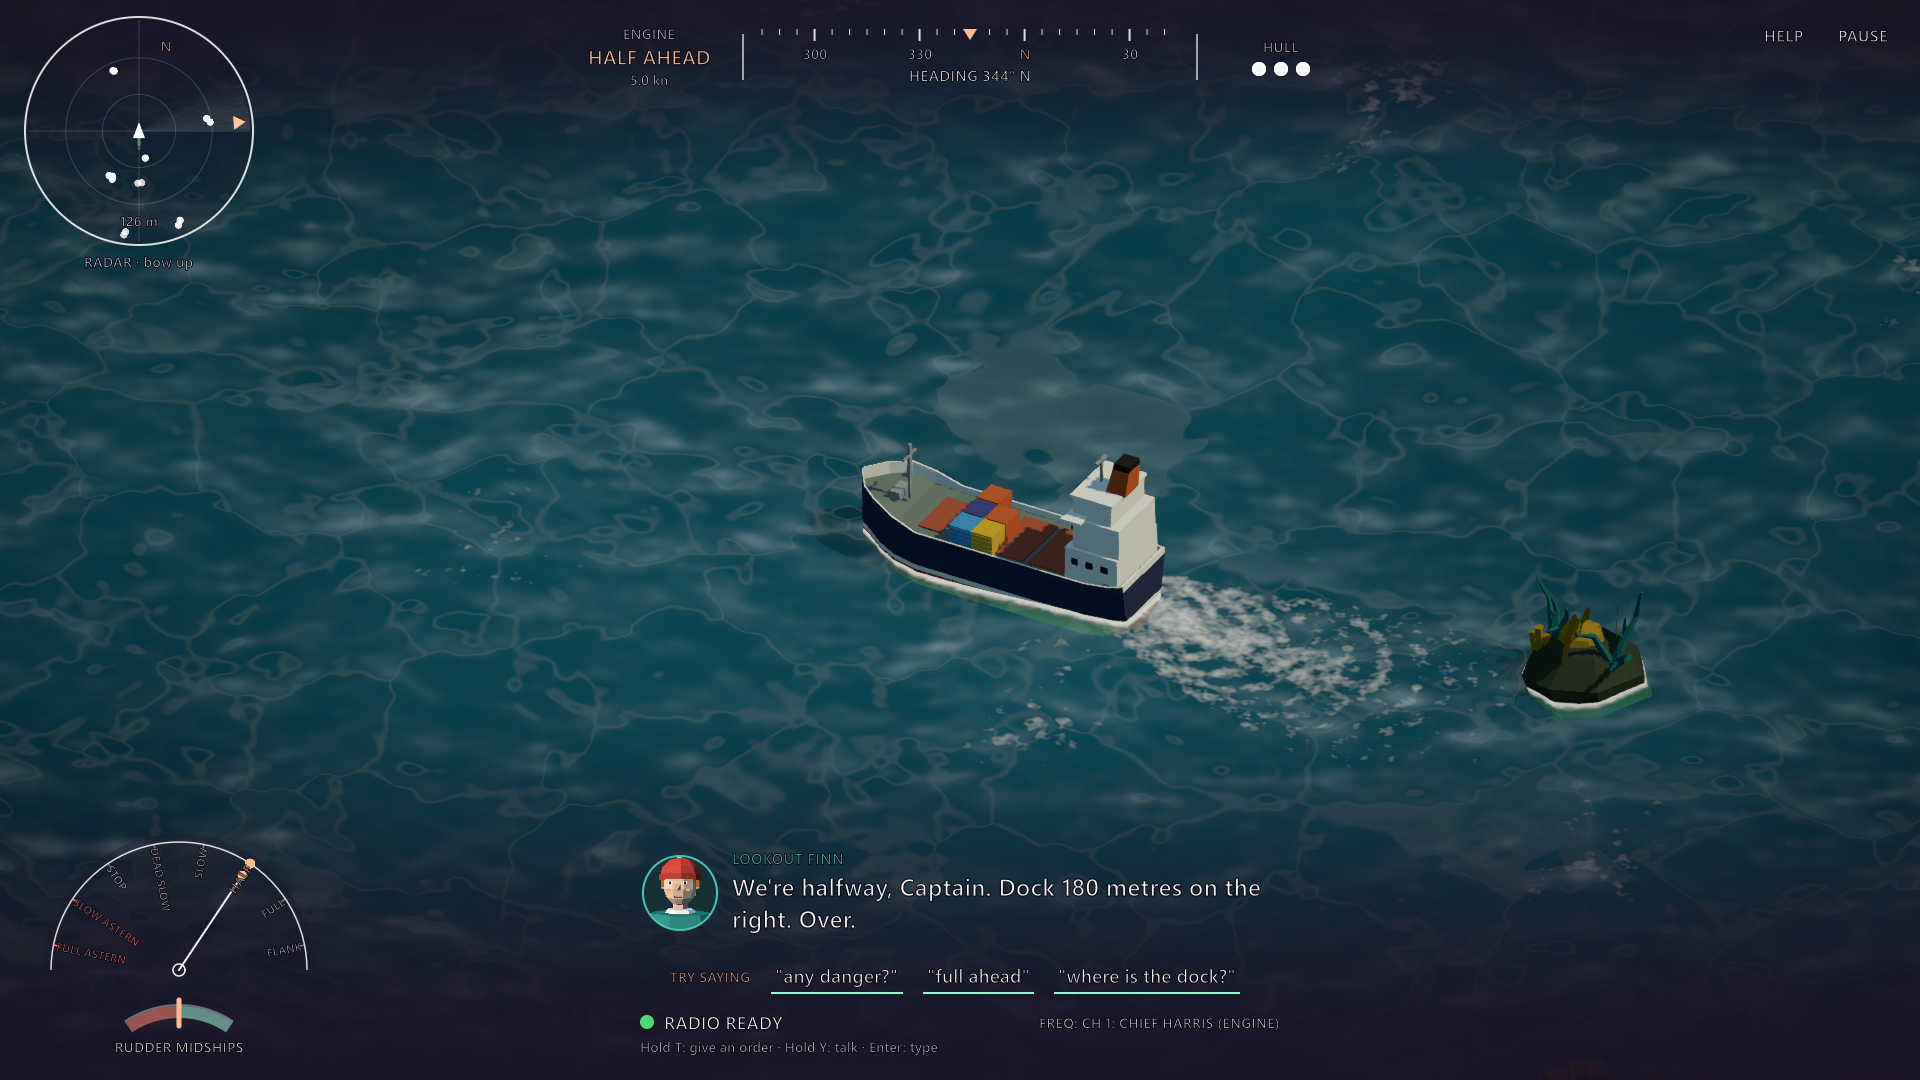
\includegraphics[width=0.8\textwidth]{Document/GameDev/images/StartUI.png}
\caption{หน้าจอเล่นเกม (UI-02)}
\label{fig:wf_gameplay}
\end{figure}

จากภาพที่ \ref{fig:wf_gameplay} ผู้เล่นมองเห็นตัวเรือ สภาพแวดล้อมทางทะเล และตำแหน่งของสิ่งกีดขวางโดยรอบจากมุมมองไอโซเมตริก องค์ประกอบบนหน้าจอมีดังนี้
\begin{itemize}
    \item แถบด้านบนกลางแสดงคำสั่งเครื่องยนต์และความเร็ว แถบเข็มทิศบอกองศาหัวเรือ และความทนทานของตัวเรือเป็นจุดกลมเรียงกัน (HULL) ซึ่งลดลงหนึ่งจุดเมื่อชน
    \item มุมซ้ายบนเป็นเรดาร์ที่แสดงร่องน้ำ แนวหิน ทุ่นระเบิด และท่าปลายทาง เพื่อช่วยประเมินสถานการณ์ล่วงหน้า
    \item มุมซ้ายล่างเป็นคันโทรเลขเครื่องยนต์ (Engine Telegraph) และตัวแสดงมุมหางเสือ (Rudder Angle Indicator)
    \item ด้านล่างกลางมีคำแนะนำประโยคที่ควรพูด (Try Saying) คำบรรยายบทพูดของลูกเรือ และกล่องวิทยุแสดงสถานะขณะรับเสียง (SENDING ORDER) และขณะแปลงเสียง (DECODING...)
\end{itemize}
กล่องวิทยุช่วยให้ผู้เล่นรู้ว่าควรเริ่มพูดหรือรอเมื่อใด จึงบริหารเวลาในการสื่อสารได้

\subsubsection{UI-03: หน้าจออู่ต่อเรือ (Shipyard)}

หน้าจออู่ต่อเรือเป็นจุดเริ่มของการเดินเรือแต่ละรอบ ดังภาพที่ \ref{fig:ui_shipyard}

\begin{figure}[!htbp]
\centering
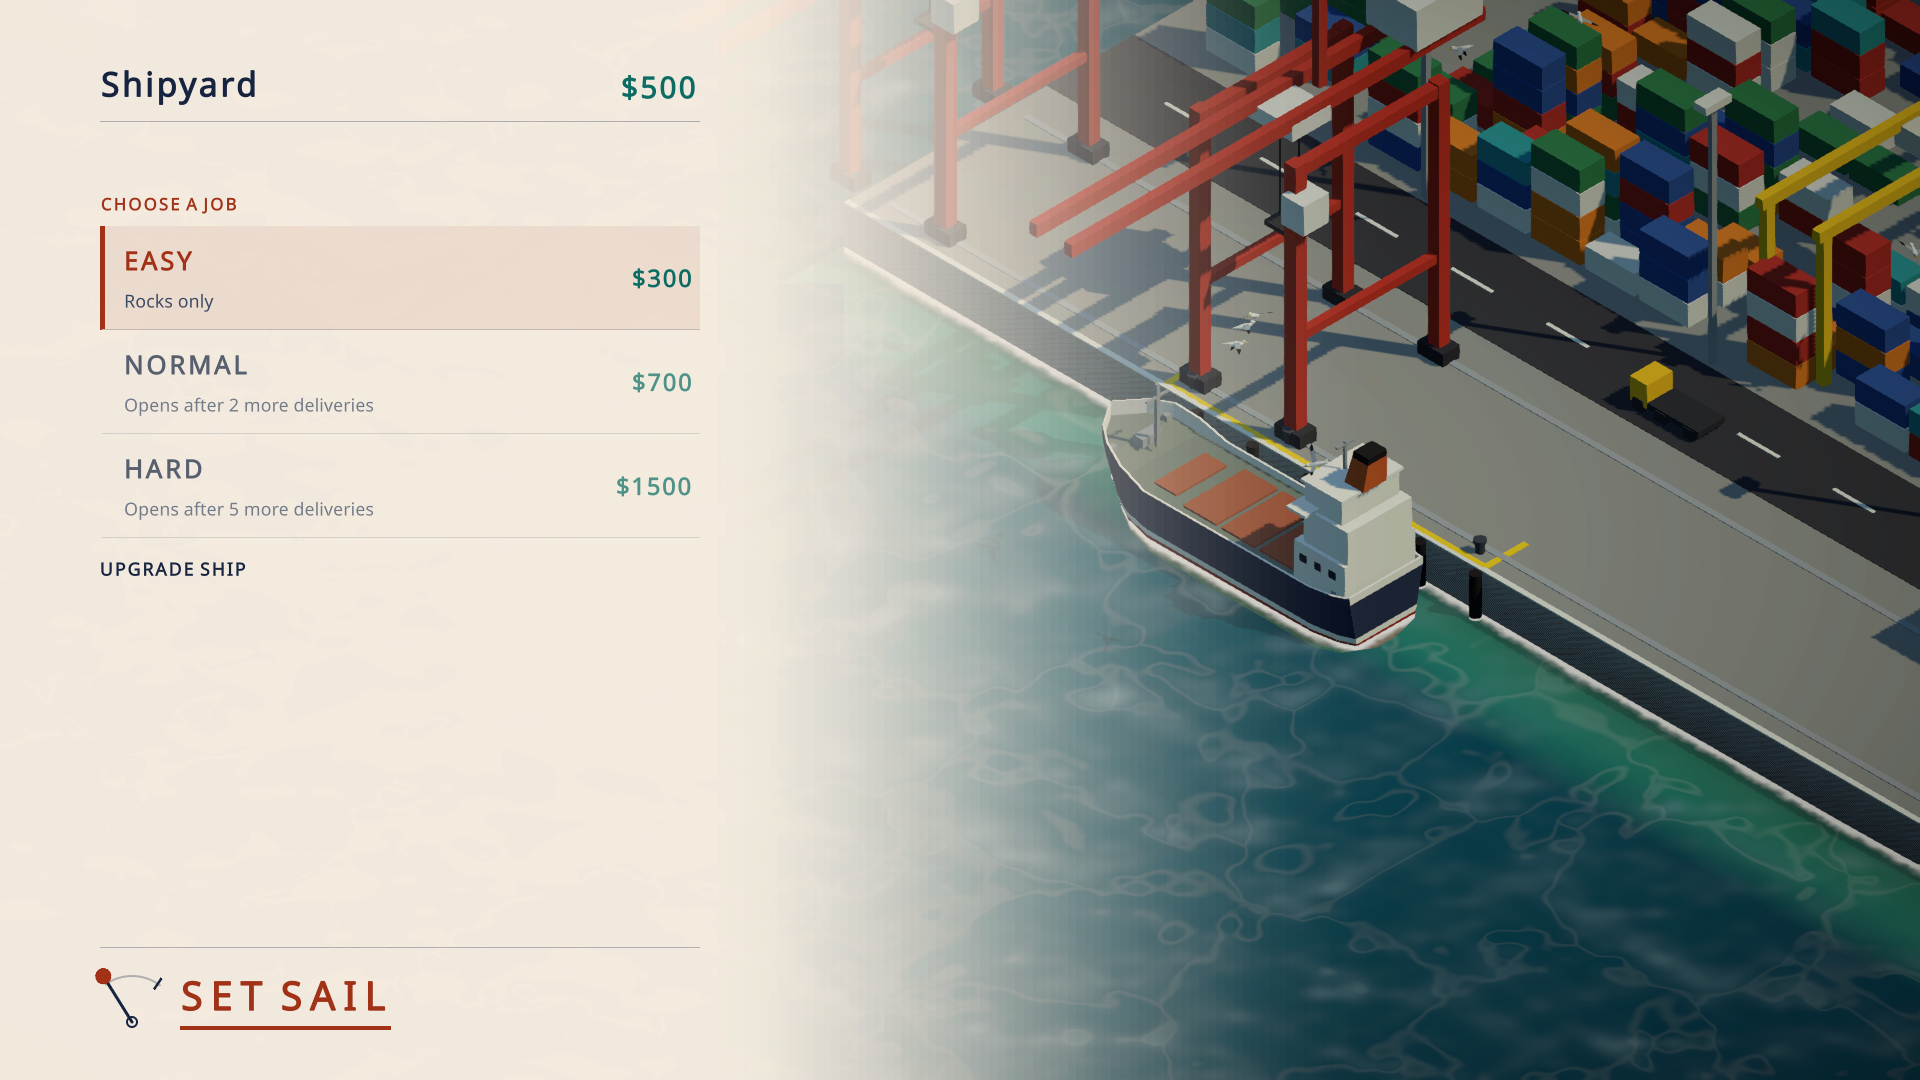
\includegraphics[width=0.8\textwidth]{Document/GameDev/images/Shipyard.png}
\caption{หน้าจออู่ต่อเรือ (UI-03)}
\label{fig:ui_shipyard}
\end{figure}

จากภาพที่ \ref{fig:ui_shipyard} ด้านซ้ายแสดงยอดเงินและรายการงานขนส่ง 3 ระดับ พร้อมค่าตอบแทนและเงื่อนไขการปลดล็อก ส่วนปุ่มอัปเกรดเรือเปิดรายการอัปเกรด 5 ด้าน ได้แก่ เครื่องยนต์ หางเสือ ยามระวังหน้า ตัวเรือ และลูกเรือ ซึ่งต้องใช้ทั้งเงินและใบรับรองทักษะภาษาที่ได้จากการใช้รูปประโยคมาตรฐาน และปุ่ม SET SAIL เริ่มการเดินเรือ ด้านขวาแสดงเรือของผู้เล่นที่ท่าเรือ

\subsubsection{UI-04: หน้าจอสรุปผล (Result Screen)}

หน้าจอสรุปผลแสดงหลังจบการเดินเรือทุกรอบ ดังภาพที่ \ref{fig:ui_result}

\begin{figure}[!htbp]
\centering
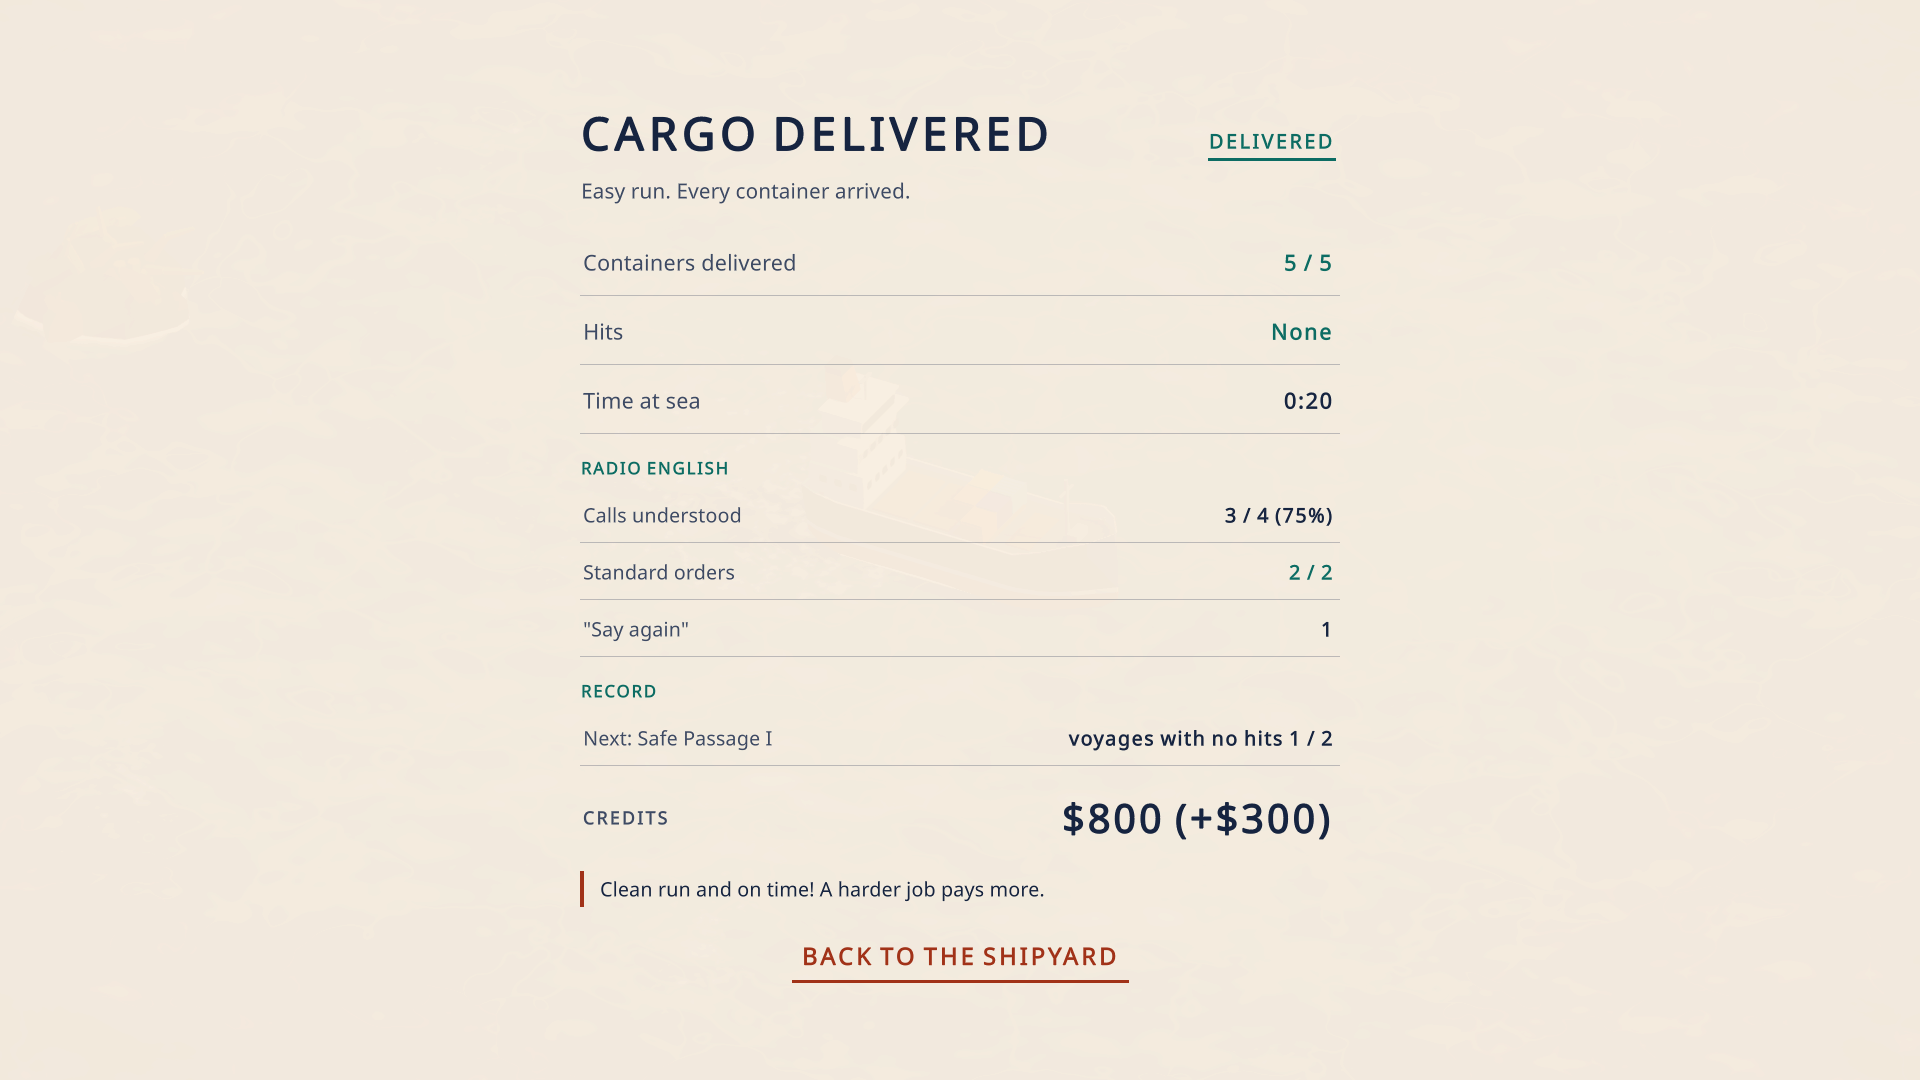
\includegraphics[width=0.8\textwidth]{Document/GameDev/images/Victory.png}
\caption{หน้าจอสรุปผล (UI-04)}
\label{fig:ui_result}
\end{figure}

จากภาพที่ \ref{fig:ui_result} หัวข้อแสดง CARGO DELIVERED (หรือ MISSION COMPLETE ในโหมดเนื้อเรื่อง) ส่วนบนแสดงผลการเดินเรือ ได้แก่ จำนวนตู้สินค้าที่ส่งถึง จำนวนครั้งที่ชน และเวลาที่ใช้ ส่วน RADIO ENGLISH สรุปการสื่อสาร ได้แก่ สัดส่วนคำสั่งที่ลูกเรือเข้าใจ จำนวนคำสั่งมาตรฐาน จำนวนครั้งที่ลูกเรือขอให้พูดซ้ำ เวลาเฉลี่ยในการสั่งหลังได้รับคำเตือน และจำนวนคำสั่งฉุกเฉินที่ทันเวลา โดยแต่ละบรรทัดแสดงเมื่อมีข้อมูลในรอบนั้น ส่วน RECORD แสดงความคืบหน้าของใบรับรองถัดไป และด้านล่างแสดงเงินที่ได้รับพร้อมคำแนะนำสำหรับรอบถัดไป หากเรืออับปาง หัวข้อจะเปลี่ยนเป็น SHIP LOST และแสดงจำนวนตู้สินค้าที่เสียและค่าลากเรือกลับท่าแทนจำนวนตู้สินค้าที่ส่งถึง

\subsubsection{UI-05: เมนูหยุดเกม (Pause)}

เมื่อกดปุ่ม PAUSE หรือ Esc ระหว่างเดินเรือ เกมจะหยุดและแสดงเมนูหยุดเกมทับหน้าจอเล่นเกม ดังภาพที่ \ref{fig:ui_pause}

\begin{figure}[!htbp]
\centering
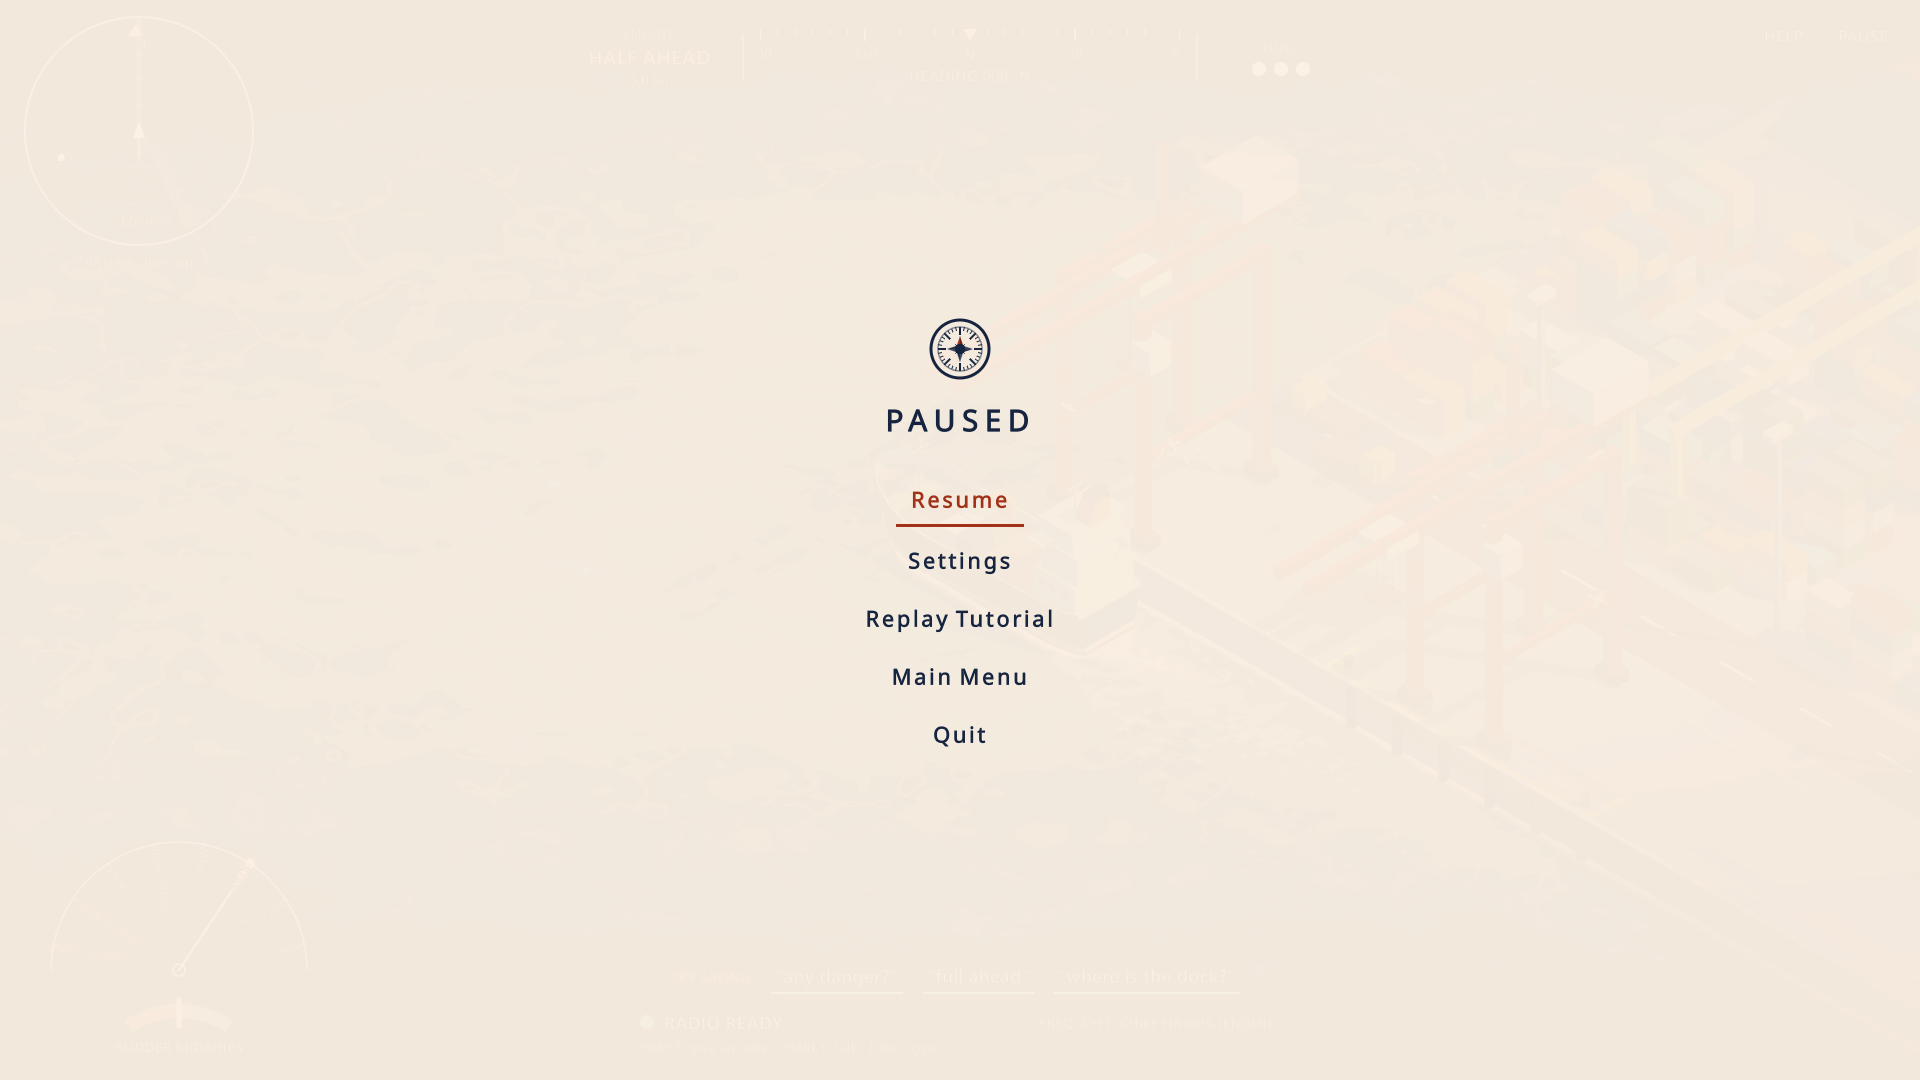
\includegraphics[width=0.8\textwidth]{Document/GameDev/images/Pause.png}
\caption{เมนูหยุดเกม (UI-05)}
\label{fig:ui_pause}
\end{figure}

จากภาพที่ \ref{fig:ui_pause} เมนูหยุดเกมประกอบด้วย Resume Settings Replay Tutorial Main Menu และ Quit และเกมยกเลิกการบันทึกเสียงที่ค้างอยู่เมื่อหยุดเกม

\subsubsection{UI-06: หน้าจอตั้งค่า (Settings)}

หน้าจอตั้งค่าเปิดได้ทั้งจากหน้าจอหลักและเมนูหยุดเกม ดังภาพที่ \ref{fig:ui_settings}

\begin{figure}[!htbp]
\centering
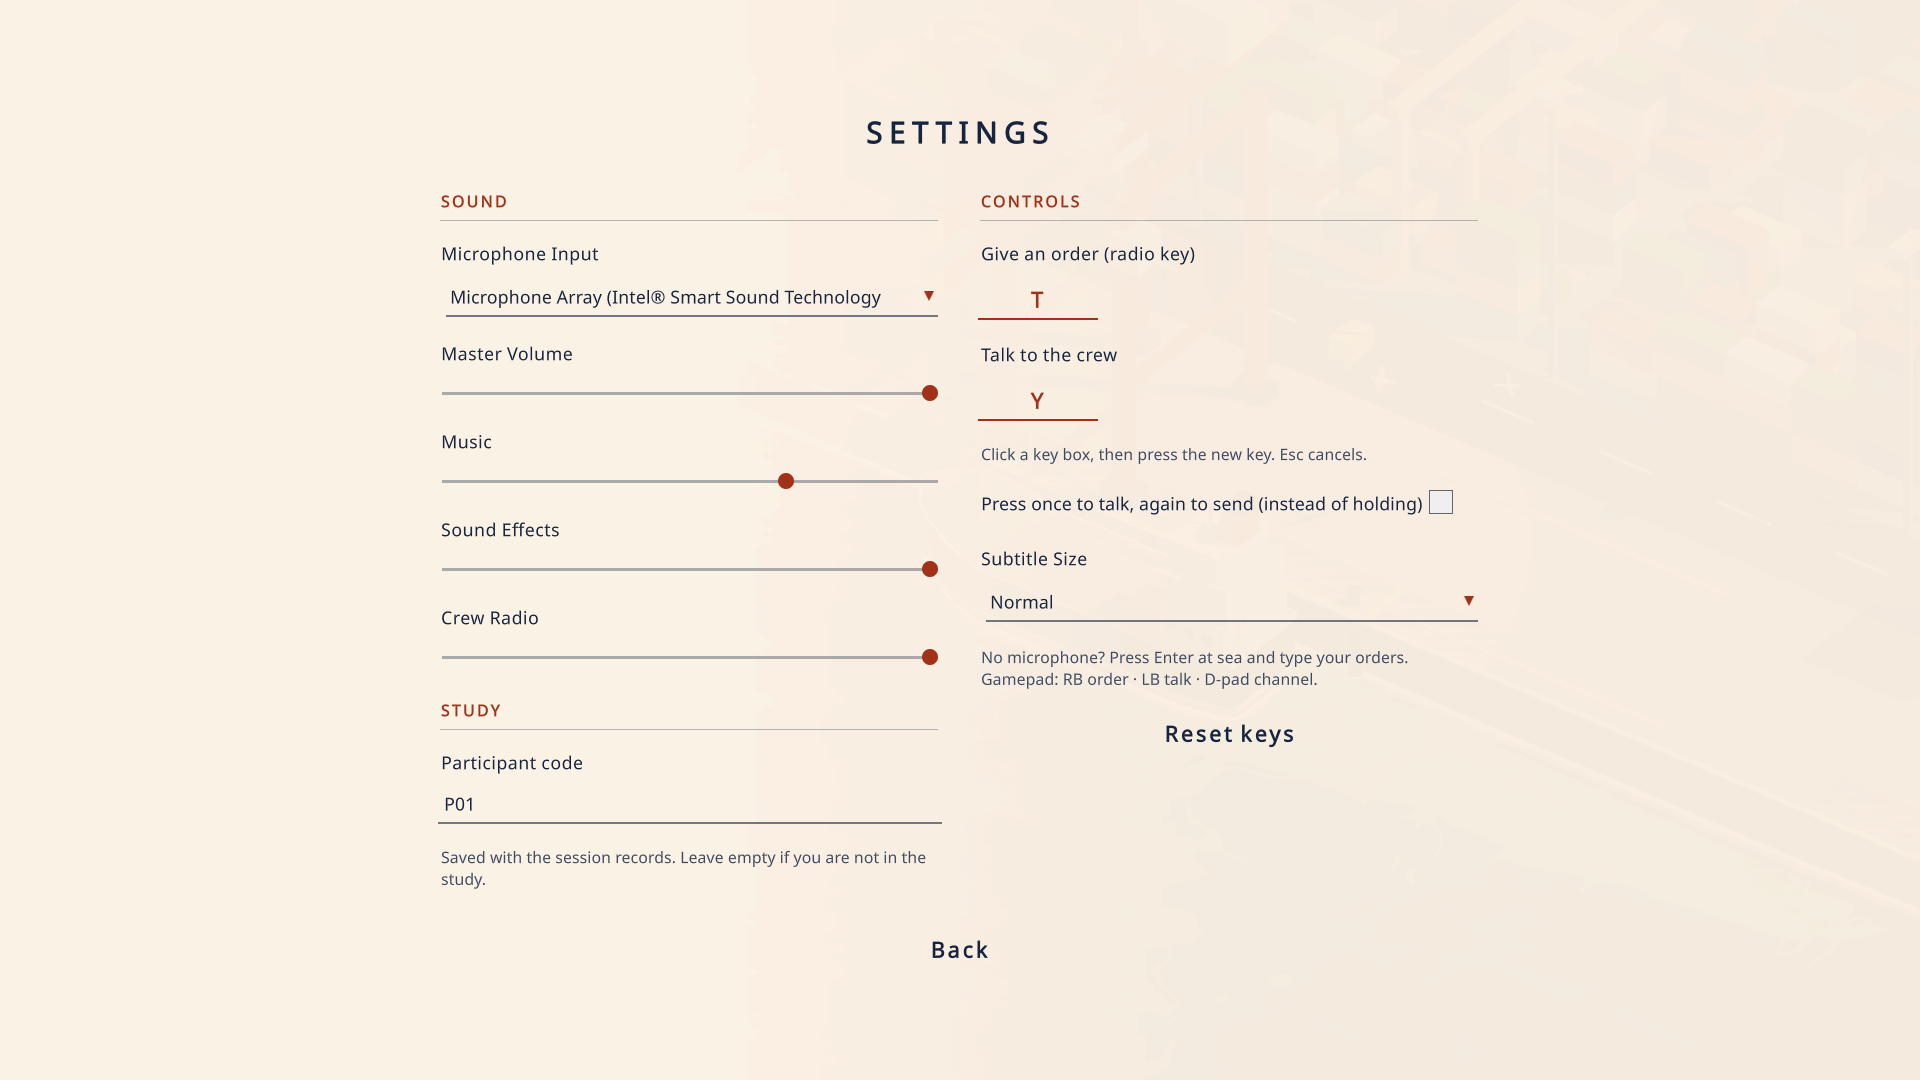
\includegraphics[width=0.8\textwidth]{Document/GameDev/images/Settings.png}
\caption{หน้าจอตั้งค่า (UI-06)}
\label{fig:ui_settings}
\end{figure}

จากภาพที่ \ref{fig:ui_settings} หน้าจอตั้งค่าแบ่งเป็น 3 ส่วน ได้แก่ SOUND (เลือกไมโครโฟน ระดับเสียงรวม ดนตรี เสียงประกอบ และเสียงวิทยุของลูกเรือ) CONTROLS (ปุ่มสั่งการ ปุ่มสนทนา โหมดกดครั้งเดียวเพื่อพูดและกดอีกครั้งเพื่อส่งแทนการกดค้าง และขนาดคำบรรยาย พร้อมคำแนะนำการพิมพ์คำสั่งและการใช้จอยเกม) และ STUDY (รหัสผู้เข้าร่วม ซึ่งบันทึกไปพร้อมกับแฟ้มบันทึกผล และเว้นว่างได้หากไม่ได้เข้าร่วมการทดลอง)

% =============================================================
% 4.4 การออกแบบองค์ประกอบในเกม
% โครงงาน: การออกแบบและพัฒนาเกมเดินเรือด้วยระบบสั่งการด้วยเสียงเพื่อส่งเสริมทักษะการสื่อสาร
% =============================================================

\section{การออกแบบองค์ประกอบในเกม}

องค์ประกอบภายในเกมได้รับการออกแบบเพื่อสร้างสภาพแวดล้อมจำลองที่สมจริง (Immersive Environment) และเอื้อต่อการเรียนรู้และการฝึกทักษะการสื่อสารภาษาอังกฤษ โดยแบ่งองค์ประกอบออกเป็น 3 ส่วนหลัก ดังนี้

\subsection{การออกแบบตัวละครและบทบาท (Characters and Roles)}

เกมจำลองสถานการณ์การทำงานร่วมกันระหว่างสะพานเดินเรือกับห้องเครื่อง โดยแบ่งบทบาทตัวละครออกเป็น 3 ตำแหน่งหลัก ดังนี้

\begin{enumerate}[label=\arabic*)]
    \item \textbf{กัปตัน:} ตัวแทนของผู้เล่น (Player Character) เป็นผู้มีอำนาจตัดสินใจสูงสุดและเป็นผู้ออกคำสั่งภาษาอังกฤษเพียงผู้เดียว
    \item \textbf{ต้นกลเรือ:} ลูกเรือปัญญาประดิษฐ์ชื่อ Harris ประจำห้องเครื่อง ทำหน้าที่รับคำสั่งเครื่องยนต์และความเร็วจากกัปตันผ่านวิทยุช่องที่ 1 (เช่น ``Slow ahead'' ``Stop engine'' ``Full astern'') แล้วตั้งคันโทรเลขเครื่องยนต์ตามคำสั่ง พร้อมทวนคำสั่ง (Read-back) เพื่อยืนยันความเข้าใจ
    \item \textbf{พลถือท้ายและยามระวังหน้า:} ลูกเรือปัญญาประดิษฐ์ชื่อ Finn ทำหน้าที่รับคำสั่งหางเสือจากกัปตันผ่านวิทยุช่องที่ 2 (เช่น ``Starboard fifteen'' ``Midships'' ``hard-a-port'') เพื่อบังคับหางเสือ พร้อมทวนคำสั่ง และคอยเฝ้าระวังรอบตัวเรือ แจ้งเตือนภัยจากเรดาร์และระยะห่างของสิ่งกีดขวาง เพื่อให้กัปตันนำข้อมูลไปตัดสินใจ
\end{enumerate}

กัปตันเลือกช่องวิทยุเพื่อสั่งการลูกเรือแต่ละคน หากผู้เล่นส่งคำสั่งผิดช่อง เช่น สั่งหางเสือผ่านช่องของต้นกลเรือ ลูกเรือจะแจ้งให้กัปตันสั่งการกับลูกเรือที่รับผิดชอบแทน ซึ่งช่วยฝึกให้ผู้เล่นระบุผู้รับสารให้ถูกต้องตามแบบการสื่อสารบนเรือจริง

\subsection{การออกแบบอุปสรรคและสิ่งกีดขวาง (Obstacles and Hazards)}

เพื่อให้เกมมีความท้าทายและป้องกันไม่ให้ผู้เล่นท่องจำเส้นทาง โหมดเดินเรืออิสระจึงสุ่มวางสิ่งกีดขวางใหม่ทุกครั้ง ส่วนภารกิจในโหมดเนื้อเรื่องใช้แผนที่คงที่ ร่องน้ำมีชายฝั่งและแนวหินกั้นทั้งสองข้าง และมีสิ่งกีดขวางกระจายอยู่ภายในร่องน้ำ ดังนี้

\begin{itemize}
    \item \textbf{หินและแนวหินโสโครก:} กำหนดให้ผู้เล่นต้องประเมินระยะห่างและสั่งการเลี้ยวหลบให้ทันเวลา การชนแต่ละครั้งทำให้ความทนทานของตัวเรือลดลงและเสียตู้สินค้า 1 ตู้
    \item \textbf{ทุ่นระเบิด:} ปรากฏตั้งแต่งานระดับ Normal ขึ้นไป เป็นกลุ่มละ 2--3 ลูก การชนทุ่นระเบิดทำให้เสียตู้สินค้า 2 ตู้
    \item \textbf{สันดอน:} ทำให้เรือเกยตื้นโดยตัวเรือไม่เสียหาย แต่ผู้เล่นต้องสั่งถอยหรือเดินหน้าช้าเพื่อนำเรือออก
\end{itemize}

\subsection{การออกแบบกราฟิกและเสียงประกอบ (Graphic and Audio Design)}

การออกแบบด้านทัศนศิลป์และเสียงมุ่งสร้างความรู้สึกดื่มด่ำ ให้ผู้เล่นรู้สึกราวกับบัญชาการเรือจริง

\begin{itemize}
    \item \textbf{กราฟิก (Graphic):} นำเสนอในมุมมองไอโซเมตริก เพื่อให้ผู้เล่นมองเห็นตัวเรือ สภาพแวดล้อมทางทะเล และตำแหน่งของสิ่งกีดขวางโดยรอบได้อย่างชัดเจนในมุมกว้าง
    \item \textbf{เสียงแวดล้อม (Ambient Audio):} เสียงคลื่นและนกนางนวลสังเคราะห์ด้วยโค้ดขณะเล่นจึงไม่วนซ้ำ ร่วมกับเสียงเครื่องยนต์เรือที่ดังต่อเนื่อง เพื่อสร้างบรรยากาศการเดินเรือที่สมจริง
    \item \textbf{เสียงเอฟเฟกต์:} ใช้เสียงสัญญาณเตือนภัย (Alarm) จากเรดาร์เมื่อเรือเคลื่อนเข้าใกล้สิ่งกีดขวาง เพื่อกระตุ้นความตื่นตัวและสร้างความกดดันด้านเวลาให้ผู้เล่นต้องรีบออกคำสั่ง
\end{itemize}
% =============================================================
% 4.5 การออกแบบเชิงการศึกษาและการประเมินผล
% โครงงาน: การออกแบบและพัฒนาเกมเดินเรือด้วยระบบสั่งการด้วยเสียงเพื่อส่งเสริมทักษะการสื่อสาร
% =============================================================

\section{การออกแบบเชิงการศึกษาและการประเมินผล}

เนื่องจากโครงงานนี้เป็นเกมเพื่อการเรียนรู้ (Serious Game) การออกแบบจึงบูรณาการการเรียนรู้โดยใช้เกมเป็นฐาน (Digital Game-Based Learning) เข้ากับทฤษฎีการเรียนรู้ภาษา เพื่อให้ผู้เล่นได้พัฒนาทักษะเชิงปฏิบัติ~\cite{sadigzade2025} โดยแบ่งออกเป็น 2 ส่วน ดังนี้

\subsection{การออกแบบเชิงการศึกษา (Educational Design)}

การออกแบบกลไกเพื่อส่งเสริมการเรียนรู้ประกอบด้วยแนวคิดหลัก ดังนี้

\begin{enumerate}[label=\arabic*)]
    \item \textbf{การเรียนรู้ตามสถานการณ์ (Situated Learning):} ผู้เล่นไม่ได้เรียนรู้คำศัพท์จากการท่องจำ แต่เรียนรู้ผ่านการจำลองการสื่อสารทางวิทยุในการเดินเรือ เช่น การสั่งหางเสือหรือการปรับความเร็ว เพื่อให้เข้าใจภาษาในบริบทที่ใช้จริง~\cite{lave1991} ซึ่งสอดคล้องกับแนวทางการเรียนรู้โดยใช้เกมเป็นฐาน~\cite{sadigzade2025}
    \item \textbf{การลดตัวกรองทางอารมณ์ (Affective Filter Hypothesis):} สมมติฐานนี้เสนอว่าความวิตกกังวลขัดขวางการรับภาษา~\cite{krashen1982} การให้ผู้เล่นฝึกพูดสั่งการกับลูกเรือปัญญาประดิษฐ์แทนการสนทนากับมนุษย์ จึงออกแบบมาเพื่อสร้างพื้นที่ปลอดภัย (Safe Space) ลดความกลัวความผิดพลาด และบรรเทาความวิตกกังวลในการใช้ภาษาต่างประเทศ (Language Anxiety)
    \item \textbf{การเรียนรู้จากข้อผิดพลาด (Learning from Failure):} เมื่อผู้เล่นออกเสียงไม่ชัดเจน ระบบไม่ลงโทษด้วยการตัดจบทันที แต่ลูกเรือจะขอให้พูดซ้ำ และเมื่อผู้เล่นใช้รูปประโยคที่ไม่ใช่มาตรฐาน ลูกเรือจะทวนกลับด้วยรูปประโยคมาตรฐาน (Recast) ทั้งสองแบบเป็นข้อมูลป้อนกลับ (Feedback) ที่กระตุ้นให้ผู้เล่นแก้ไขการพูดด้วยตนเอง~\cite{zargham2024}
\end{enumerate}

\subsection{แนวทางการประเมินผล (Evaluation Approach)}

ผู้จัดทำออกแบบการประเมินผลให้ครอบคลุมทั้งประสิทธิภาพของเทคโนโลยีและผลด้านการเรียนรู้ของผู้เล่น ดังนี้

\begin{itemize}
    \item \textbf{การประเมินผลภายในเกม (In-game Evaluation):} ประเมินจากร้อยละของการสื่อสารที่ลูกเรือเข้าใจ จำนวนครั้งที่ลูกเรือขอให้พูดซ้ำ ความรวดเร็วในการสั่งการหลังได้รับคำเตือน จำนวนครั้งที่ชน และจำนวนคำสั่งฉุกเฉินที่ทันเวลา
    \item \textbf{การประเมินประสิทธิภาพทางเทคนิค (Technical Evaluation):} ประเมินความแม่นยำของการแปลงเสียงเป็นข้อความโดยให้ผู้เข้าร่วมแต่ละคนอ่านรายการคำสั่งมาตรฐาน 10 คำสั่ง (คำสั่งเป้าหมาย) ระหว่างการเล่น แล้วคำนวณร้อยละของคำสั่งเป้าหมายที่ระบบถอดความและแยกคำสั่งได้ถูกต้อง โดยเทียบรายการคำสั่งเป้าหมายกับคอลัมน์ข้อความที่ได้ยินและคำสั่งที่ระบบแยกได้ในแฟ้ม turns.csv ส่วนการเล่นอิสระรายงานเฉพาะร้อยละของการสื่อสารที่ลูกเรือเข้าใจ นอกจากนี้วัดความหน่วง (Latency) ตั้งแต่ผู้เล่นปล่อยปุ่มวิทยุจนเรือเริ่มตอบสนอง
    \item \textbf{การประเมินความวิตกกังวลในการพูดภาษาอังกฤษ (Speaking Anxiety Evaluation):} ผู้เล่นตอบแบบวัดความวิตกกังวลในการพูดภาษาอังกฤษ 12 ข้อ ที่ดัดแปลงจาก FLCAS~\cite{horwitz1986} ทั้งก่อนและหลังเล่นเกม เพื่อเปรียบเทียบว่าความวิตกกังวลลดลงหรือไม่
    \item \textbf{การประเมินประสบการณ์ผู้เล่น (User Experience Evaluation):} ประเมินผ่านแบบสอบถามหลังการเล่น 10 ข้อ ครอบคลุมความเข้าใจง่าย ความสมจริง การตอบกลับของลูกเรือ ประโยชน์ของคำแนะนำประโยคและการทวนด้วยรูปประโยคมาตรฐาน ความรู้สึกปลอดภัยในการพูด และความสนุก โดยแบบวัดและแบบสอบถามทั้งหมดแสดงในภาคผนวก ก และวิธีวิเคราะห์ผลอธิบายในบทที่ 3
\end{itemize}
% =============================================================
% 4.x การออกแบบข้อมูล
% =============================================================

\section{การออกแบบข้อมูล}

เกมเป็นเกมผู้เล่นเดี่ยวที่ทำงานบนเครื่องของผู้เล่นเพียงเครื่องเดียว จึงไม่ใช้ระบบฐานข้อมูล แต่จัดเก็บข้อมูล 2 กลุ่ม ได้แก่ (1) ข้อมูลความก้าวหน้าและการตั้งค่า ซึ่งเก็บด้วย PlayerPrefs ของ Unity ในรูปแบบคู่คีย์และค่า (Key-Value) และ (2) ข้อมูลบันทึกผลการทดลอง ซึ่งเก็บเป็นแฟ้ม CSV 3 แฟ้ม เพื่อให้ผู้ดำเนินการทดลองนำไปวิเคราะห์ด้วยโปรแกรมตารางคำนวณหรือโปรแกรมสถิติได้โดยตรง ดังภาพที่ \ref{fig:data_overview}

\begin{figure}[!htbp]
\centering
\begin{mermaid}
graph LR
    subgraph Game["เกม (Unity)"]
        GS["GameSession / Progression"]
        ST["StoryProgress"]
        SS["SettingsService"]
        RL["ResearchLog"]
    end

    subgraph Prefs["PlayerPrefs (Windows Registry)"]
        P1["career.*"]
        P2["progress.*"]
        P3["story.done.*"]
        P4["การตั้งค่า"]
    end

    subgraph Files["แฟ้ม CSV (Sessions)"]
        F1["turns.csv"]
        F2["voyages.csv"]
        F3["emergencies.csv"]
    end

    GS --> P1
    GS --> P2
    ST --> P3
    SS --> P4
    RL --> F1
    RL --> F2
    RL --> F3
\end{mermaid}
\caption{ภาพรวมการจัดเก็บข้อมูลของเกม}
\label{fig:data_overview}
\end{figure}

\subsection{ข้อมูลความก้าวหน้าของผู้เล่น}

ข้อมูลความก้าวหน้าบันทึกทุกครั้งที่ผู้เล่นจบการเดินเรือหรือซื้ออัปเกรด ดังตารางที่ \ref{tab:data_progress}

\begin{table}[!htbp]
\centering
\caption{คีย์ข้อมูลความก้าวหน้าของผู้เล่น}
\label{tab:data_progress}
\begin{tabular}{|L{4.46cm}|L{1.55cm}|L{7.27cm}|}
\hline
\textbf{คีย์} & \textbf{ชนิด} & \textbf{ความหมาย} \\
\hline
\texttt{career.\allowbreak credits} & int & เงินสะสมของผู้เล่น \\ \hline
\texttt{career.\allowbreak engine}, \texttt{career.\allowbreak helm}, \texttt{career.\allowbreak lookout}, \texttt{career.\allowbreak plating}, \texttt{career.\allowbreak crew} & int & ระดับอัปเกรดของเครื่องยนต์ หางเสือ การเฝ้าระวัง ตัวเรือ และลูกเรือ \\ \hline
\texttt{career.\allowbreak hull} & int & ความทนทานของตัวเรือที่เหลืออยู่ \\ \hline
\texttt{career.\allowbreak delivered}, \texttt{career.\allowbreak voyages} & int & จำนวนงานที่ส่งสำเร็จ และจำนวนการเดินเรือทั้งหมด \\ \hline
\texttt{career.\allowbreak job} & string & ระดับงานขนส่งที่เลือกล่าสุด (EASY, NORMAL, HARD) \\ \hline
\texttt{career.\allowbreak atsea} & int & ผู้เล่นออกจากเกมระหว่างเดินเรือหรือไม่ (1 = ใช่) \\ \hline
\texttt{progress.\allowbreak skill.\allowbreak <ทักษะ>} & int & จำนวนครั้งที่ใช้ทักษะภาษาแต่ละด้าน ได้แก่ EngineOrders, HelmOrders, HelmDegrees, Questions, CrewTalk, CleanVoyages, ClearVoyages, Emergencies \\ \hline
\texttt{progress.\allowbreak cert.\allowbreak <รหัส>} & int & ได้รับใบรับรองแล้วหรือไม่ (1 = ได้รับ) ใช้ปลดล็อกการอัปเกรด \\ \hline
\texttt{story.\allowbreak done.\allowbreak <บท-ภารกิจ>} & int & ภารกิจในโหมดเนื้อเรื่องที่ผ่านแล้ว เช่น \texttt{story.\allowbreak done.1-2} \\ \hline
\texttt{tutorial\_\allowbreak done}, \texttt{tutorial\_\allowbreak step} & int & เล่นบทฝึกสอนจบแล้วหรือไม่ และขั้นตอนล่าสุดที่เล่นถึง \\
\hline
\end{tabular}
\end{table}

\subsection{ข้อมูลการตั้งค่า}

ข้อมูลการตั้งค่าบันทึกเมื่อผู้เล่นเปลี่ยนค่าในหน้าตั้งค่า ดังตารางที่ \ref{tab:data_settings}

\begin{table}[!htbp]
\centering
\caption{คีย์ข้อมูลการตั้งค่า}
\label{tab:data_settings}
\begin{tabular}{|L{4.46cm}|L{1.55cm}|L{7.27cm}|}
\hline
\textbf{คีย์} & \textbf{ชนิด} & \textbf{ความหมาย} \\
\hline
\texttt{Selected\allowbreak Microphone} & string & ชื่ออุปกรณ์ไมโครโฟนที่เลือก \\ \hline
\texttt{MasterVolume}, \texttt{MusicVolume}, \texttt{EffectsVolume}, \texttt{RadioVolume} & float & ระดับเสียงรวม ดนตรี เสียงประกอบ และเสียงวิทยุ (0--1) \\ \hline
\texttt{ToggleToTalk} & int & 0 = กดค้างเพื่อพูด, 1 = กดครั้งแรกเพื่อเริ่ม กดอีกครั้งเพื่อส่ง \\ \hline
\texttt{SubtitleScale} & float & ขนาดคำบรรยายบทพูดของลูกเรือ \\ \hline
\texttt{Binding.\allowbreak CommandPtt}, \texttt{Binding.\allowbreak ConversationPtt} & string & ปุ่มสั่งการและปุ่มสนทนาที่ผู้เล่นกำหนดเอง (JSON) \\ \hline
\texttt{research.\allowbreak participant} & string & รหัสผู้เข้าร่วมการทดลอง (ไม่เกิน 24 ตัวอักษร) \\
\hline
\end{tabular}
\end{table}

\subsection{แฟ้มบันทึกผลการทดลอง}

แฟ้มบันทึกผลเก็บที่โฟลเดอร์ \texttt{Sessions} ในโฟลเดอร์ข้อมูลของเกมบนเครื่องผู้เล่น ทุกแถวขึ้นต้นด้วยคอลัมน์ร่วม ได้แก่ \texttt{session} (วันเวลาที่เปิดเกม), \texttt{participant} (รหัสผู้เข้าร่วม), \texttt{voyage} (ลำดับการเดินเรือ), \texttt{mission} (ชื่อภารกิจหรืองาน) และ \texttt{time\_utc} (เวลาที่บันทึก) ส่วนคอลัมน์เฉพาะของแต่ละแฟ้มแสดงดังตารางที่ \ref{tab:data_turns}--\ref{tab:data_emergencies}

\begin{table}[!htbp]
\centering
\caption{โครงสร้างแฟ้ม turns.csv (หนึ่งแถวต่อการสื่อสารหนึ่งครั้ง)}
\label{tab:data_turns}
\begin{tabular}{|L{4.90cm}|L{8.80cm}|}
\hline
\textbf{คอลัมน์} & \textbf{ความหมาย} \\
\hline
\texttt{input}, \texttt{key} & พูดหรือพิมพ์ (voice, typed) และปุ่มที่ใช้ (order = T, talk = Y) \\ \hline
\texttt{speech\_s} & ความยาวเสียงที่บันทึก (วินาที) \\ \hline
\texttt{heard} & ข้อความที่ Whisper ถอดได้ หรือข้อความที่พิมพ์ \\ \hline
\texttt{outcome} & ผลลัพธ์ ได้แก่ order, answered, word, unclear, no reply (ไม่มีลูกเรือตอบ), rejected:none (ไม่มีข้อความ) หรือ rejected:<เหตุผล> \\ \hline
\texttt{route} & ส่วนที่เข้าใจคำสั่ง ได้แก่ local (ตัวแยกคำสั่ง), classifier (GPT จำแนกเจตนา บันทึกแม้ไม่ได้เรียกบริการจริง), chat (GPT สนทนา) \\ \hline
\texttt{actions}, \texttt{standard}, \texttt{taught} & คำสั่งที่ทำ, ใช้รูปประโยคมาตรฐานหรือไม่ และรูปประโยคมาตรฐานที่ลูกเรือทวนให้ \\ \hline
\texttt{reply\_by}, \texttt{reply} & ลูกเรือที่ตอบ และข้อความที่ตอบ \\ \hline
\texttt{stt\_ms} & เวลาตั้งแต่ปล่อยปุ่มจนได้ข้อความ (มิลลิวินาที) \\ \hline
\texttt{reply\_ms}, \texttt{total\_ms} & เวลาตั้งแต่ได้ข้อความจนลูกเรือตอบ และเวลารวมตั้งแต่ปล่อยปุ่มจนลูกเรือตอบ \\ \hline
\texttt{ship\_ms} & เวลาตั้งแต่ปล่อยปุ่มจนเรือเริ่มทำตามคำสั่ง \\ \hline
\texttt{danger}, \texttt{hull} & มีสิ่งกีดขวางใกล้เรือขณะสั่งหรือไม่ และความทนทานของเรือขณะนั้น \\
\hline
\end{tabular}
\end{table}

\begin{table}[!htbp]
\centering
\caption{โครงสร้างแฟ้ม voyages.csv (หนึ่งแถวต่อการเดินเรือหนึ่งรอบ)}
\label{tab:data_voyages}
\begin{tabular}{|L{4.90cm}|L{8.80cm}|}
\hline
\textbf{คอลัมน์} & \textbf{ความหมาย} \\
\hline
\texttt{delivered}, \texttt{seconds}, \texttt{par\_seconds} & ส่งสินค้าสำเร็จหรือไม่ เวลาที่ใช้ และเวลามาตรฐานของด่าน \\ \hline
\texttt{hits}, \texttt{mine\_hits} & จำนวนครั้งที่ชนสิ่งกีดขวาง และจำนวนครั้งที่ชนทุ่นระเบิด \\ \hline
\texttt{cargo\_loaded}, \texttt{cargo\_delivered} & จำนวนตู้สินค้าที่บรรทุก และจำนวนที่ส่งถึง \\ \hline
\texttt{calls}, \texttt{understood}, \texttt{understood\_pct} & จำนวนครั้งที่สื่อสาร จำนวนที่ลูกเรือเข้าใจ และร้อยละที่เข้าใจ \\ \hline
\texttt{orders}, \texttt{standard\_orders} & จำนวนคำสั่ง และจำนวนคำสั่งที่ใช้รูปประโยคมาตรฐาน \\ \hline
\texttt{say\_again}, \texttt{words\_asked} & จำนวนครั้งที่ลูกเรือขอให้พูดซ้ำ และจำนวนคำศัพท์ที่ผู้เล่นถามความหมาย \\ \hline
\texttt{avg\_reaction\_s} & เวลาเฉลี่ยตั้งแต่ลูกเรือเตือนภัยจนผู้เล่นออกคำสั่ง \\ \hline
\texttt{practise} & รูปประโยคที่แนะนำให้ผู้เล่นฝึกต่อ \\ \hline
\texttt{avg\_stt\_ms}, \texttt{avg\_total\_ms}, \texttt{avg\_ship\_ms} & ค่าเฉลี่ยของเวลาตอบสนองในรอบนั้น \\ \hline
\texttt{emergencies}, \texttt{emergencies\_saved} & จำนวนสถานการณ์ฉุกเฉิน และจำนวนที่ผู้เล่นหลบได้ทัน \\
\hline
\end{tabular}
\end{table}

\begin{table}[!htbp]
\centering
\caption{โครงสร้างแฟ้ม emergencies.csv (หนึ่งแถวต่อสถานการณ์ฉุกเฉินหนึ่งครั้ง)}
\label{tab:data_emergencies}
\begin{tabular}{|L{4.90cm}|L{8.80cm}|}
\hline
\textbf{คอลัมน์} & \textbf{ความหมาย} \\
\hline
\texttt{hazard}, \texttt{distance\_m} & ชนิดสิ่งกีดขวาง และระยะห่างเมื่อเริ่มสถานการณ์ (เมตร) \\ \hline
\texttt{window\_s} & เวลาที่ผู้เล่นมีในการออกคำสั่ง (วินาที) \\ \hline
\texttt{outcome} & ผลลัพธ์ ได้แก่ saved (หลบทัน), hit (ชน), cleared (พ้นอันตรายเอง) หรือ ended (ภารกิจจบก่อน) \\ \hline
\texttt{reaction\_ms}, \texttt{tries} & เวลาจริงตั้งแต่เริ่มสถานการณ์จนออกคำสั่งที่ถูกต้อง (รวมเวลาบันทึกและแปลงเสียง ขณะที่ \texttt{window\_s} ไม่นับเวลาดังกล่าว) และจำนวนครั้งที่พูด \\ \hline
\texttt{standard}, \texttt{said} & ใช้รูปประโยคมาตรฐานหรือไม่ และข้อความที่ผู้เล่นพูด \\
\hline
\end{tabular}
\end{table}

จากตารางที่ \ref{tab:data_turns}--\ref{tab:data_emergencies} ข้อมูลที่บันทึกใช้รหัสผู้เข้าร่วมและไม่มีแฟ้มเสียง จึงไม่บันทึกชื่อจริงโดยตรง แต่คอลัมน์ \texttt{heard} อาจมีคำที่ผู้เล่นพูดเอง ผู้จัดทำจะตรวจและลบข้อมูลที่ระบุตัวตนได้ก่อนวิเคราะห์ เพื่อคุ้มครองความเป็นส่วนตัวของกลุ่มตัวอย่าง หากเขียนแฟ้มไม่สำเร็จ ระบบจะบันทึกข้อผิดพลาดเพียงครั้งเดียวและให้เกมเล่นต่อได้ตามปกติ

% =============================================================
% 4.x การออกแบบการเชื่อมต่อบริการ
% =============================================================

\section{การออกแบบการเชื่อมต่อบริการ}

เกมเชื่อมต่อกับส่วนประมวลผลภายนอกตัวเกม 2 ส่วน ได้แก่ โมเดลการรู้จำเสียง Whisper ซึ่งทำงานภายในเครื่องของผู้เล่น และบริการ OpenAI Chat Completions ซึ่งเรียกใช้ผ่านอินเทอร์เน็ต โดยออกแบบให้คำสั่งที่ตัวแยกคำสั่งเข้าใจได้ไม่ต้องเรียกบริการภายนอกเลย บริการ OpenAI จึงจะเรียกใช้เฉพาะเมื่อจำเป็น ดังตารางที่ \ref{tab:services}

\begin{table}[!htbp]
\centering
\caption{บริการที่เกมเชื่อมต่อ}
\label{tab:services}
\begin{tabular}{|L{3.09cm}|L{2.44cm}|L{2.25cm}|L{5.06cm}|}
\hline
\textbf{บริการ} & \textbf{ผู้เรียกใช้} & \textbf{ตำแหน่ง} & \textbf{ใช้เมื่อ} \\
\hline
Whisper (whisper.cpp) & RadioMic & ภายในเครื่อง & ทุกครั้งที่ผู้เล่นส่งเสียงพูด \\ \hline
OpenAI: จำแนกเจตนา & IntentClassifier & อินเทอร์เน็ต & ตัวแยกคำสั่งไม่พบคำสั่งที่ชัดเจน และการเทียบคำแบบใกล้เคียงภายในเครื่องไม่ผ่านเกณฑ์ \\ \hline
OpenAI: สนทนา & OpenAIClient & อินเทอร์เน็ต & ผู้เล่นกดปุ่มสนทนา (Y) ถามคำถามที่ตอบจากข้อมูลในเกมไม่ได้ หรือตัวจำแนกเจตนาไม่ได้คำสั่ง \\
\hline
\end{tabular}
\end{table}

\subsection{การตั้งค่าโมเดลการรู้จำเสียง}

โมเดล Whisper เรียกผ่านแพ็กเกจ whisper.unity โดยตั้งค่าให้เหมาะกับคำสั่งการเดินเรือภาษาอังกฤษสั้น ๆ ดังตารางที่ \ref{tab:whisper_config}

\begin{table}[!htbp]
\centering
\caption{การตั้งค่าโมเดลการรู้จำเสียง}
\label{tab:whisper_config}
\begin{tabular}{|L{4.00cm}|L{9.70cm}|}
\hline
\textbf{รายการ} & \textbf{ค่าที่ใช้และเหตุผล} \\
\hline
โมเดล & \texttt{ggml-base.\allowbreak en.\allowbreak bin} โมเดลขนาด base สำหรับภาษาอังกฤษเท่านั้น สมดุลระหว่างความแม่นยำและความเร็วบนซีพียู \\ \hline
ภาษา & \texttt{en} และปิดการแปลภาษา เนื่องจากต้องการข้อความภาษาอังกฤษตามที่ผู้เล่นพูดจริง \\ \hline
การประมวลผล & เปิดใช้การ์ดจอ (GPU) ผ่าน Vulkan ซึ่งเร็วกว่าการใช้ซีพียูประมาณ 27 เท่าบนเครื่องทดสอบ (ตารางที่ \ref{tab:gpu_bench}) หากเครื่องไม่มีการ์ดจอที่รองรับ whisper.cpp จะใช้ซีพียูแทน \\ \hline
ข้อความนำ (Initial Prompt) & ``Captain to crew. Port, starboard, midships, slow ahead, half ahead, full ahead, astern, stop, any danger, where is the dock.'' เพื่อให้โมเดลถอดคำศัพท์การเดินเรือได้ถูกต้องขึ้น \\ \hline
การตรวจจับเสียงพูด & เปิดใช้ VAD (Voice Activity Detection) \\ \hline
ความยาวเสียง & 0.35--8 วินาที และเติมช่วงเงียบท้ายเสียงก่อนส่งเข้าโมเดล เพื่อไม่ให้ประโยคสั้นมากถูกปฏิเสธ \\
\hline
\end{tabular}
\end{table}

\subsection{การเรียกบริการ OpenAI}

การเรียกบริการทั้ง 2 แบบใช้ปลายทาง \texttt{POST} \url{https://api.openai.com/v1/chat/completions} ด้วยโมเดล GPT-4o mini แต่ตั้งค่าต่างกันตามหน้าที่ ดังตารางที่ \ref{tab:openai_params}

\begin{table}[!htbp]
\centering
\caption{ค่าพารามิเตอร์การเรียกบริการ OpenAI}
\label{tab:openai_params}
\begin{tabular}{|L{3.49cm}|L{4.56cm}|L{5.23cm}|}
\hline
\textbf{พารามิเตอร์} & \textbf{จำแนกเจตนา} & \textbf{สนทนา} \\
\hline
\texttt{model} & gpt-4o-mini & gpt-4o-mini \\ \hline
\texttt{temperature} & 0 (ให้ผลเหมือนเดิมทุกครั้ง) & 0.6 (คำตอบเป็นธรรมชาติ) \\ \hline
\texttt{top\_\allowbreak p} & -- & 0.9 \\ \hline
\texttt{frequency\_\allowbreak penalty} & -- & 0.15 \\ \hline
\texttt{max\_\allowbreak tokens} & -- & 60 (คำตอบสั้นแบบวิทยุ) \\ \hline
\texttt{response\_\allowbreak format} & \texttt{json\_\allowbreak object} & ข้อความปกติ \\ \hline
เวลารอสูงสุด & 6 วินาที & 15 วินาที \\ \hline
ข้อมูลที่ส่ง & คำสั่งของผู้เล่นและรายการชื่อคำสั่งที่เกมรองรับ & บุคลิกของลูกเรือ สถานะเรือปัจจุบัน และบทสนทนาล่าสุด 3 ครั้งของลูกเรือคนนั้น \\
\hline
\end{tabular}
\end{table}

ก่อนเรียกบริการจำแนกเจตนา ระบบจะเทียบข้อความกับรายการวลีคำสั่งภายในเครื่องก่อน หากความคล้ายคลึงตั้งแต่ 0.75 ขึ้นไป จะใช้คำสั่งนั้นทันทีโดยไม่เรียกบริการ ตัวอย่างข้อมูลรับส่งของการจำแนกเจตนาแสดงดังภาพที่ \ref{lst:intent_json}

\begin{figure}[!htbp]
\centering
\begin{lstlisting}[basicstyle=\ttfamily\footnotesize,numbers=none]
Request:
{
  "model": "gpt-4o-mini",
  "temperature": 0,
  "response_format": { "type": "json_object" },
  "messages": [
    { "role": "system", "content": "Map a ship captain's spoken order to exactly
        one action code. ... Port is left, starboard is right. ..." },
    { "role": "user", "content": "Order: \"hard to pork\"" }
  ]
}

Response (choices[0].message.content):
{ "action": "HardPort" }
\end{lstlisting}
\caption{ตัวอย่างข้อมูลรับส่งของการจำแนกเจตนา}
\label{lst:intent_json}
\end{figure}

ระบบรับเฉพาะชื่อคำสั่งที่ตรงกับรายการคำสั่งของเกม ได้แก่ คำสั่งเครื่องยนต์ (เช่น EngineSlow, EngineFullAstern) คำสั่งหางเสือ (เช่น TurnPort, RudderMidships) คำถามสถานะ (เช่น QueryHazard, QueryDestination) การยกเลิกคำสั่ง (Belay) และคำสั่งเทียบท่า (RequestDocking, MakeFast) หากได้ \texttt{None} หรือชื่อที่ไม่อยู่ในรายการ ระบบจะส่งข้อความต่อให้ลูกเรือตอบผ่านบริการสนทนา และหากไม่สำเร็จลูกเรือจะขอให้พูดซ้ำ

\subsection{การจัดการข้อผิดพลาด}

เนื่องจากการสื่อสารเป็นหัวใจของเกม ข้อผิดพลาดของบริการทุกกรณีจึงถูกแปลงเป็นพฤติกรรมที่สมจริงของลูกเรือ แทนการแสดงข้อความแจ้งข้อผิดพลาดทางเทคนิค ดังตารางที่ \ref{tab:service_errors}

\begin{table}[!htbp]
\centering
\caption{การจัดการข้อผิดพลาดของบริการ}
\label{tab:service_errors}
\begin{tabular}{|L{4.60cm}|L{9.10cm}|}
\hline
\textbf{สถานการณ์} & \textbf{การตอบสนองของเกม} \\
\hline
ไม่มีเสียงจากไมโครโฟน & แสดง ``No sound from the microphone. Check Settings.'' ที่ช่องสถานะวิทยุ \\ \hline
เสียงสั้นหรือเบาเกินไป & แสดงคำแนะนำให้กดปุ่มค้างระหว่างพูด หรือพูดดังขึ้น โดยไม่ส่งคำสั่ง \\ \hline
โมเดล Whisper ยังโหลดไม่เสร็จ & แจ้งว่าระบบเสียงยังไม่พร้อม ให้ลองใหม่อีกครั้ง \\ \hline
Whisper ถอดได้เพียงเสียงรบกวน & แจ้ง ``Didn't catch that. Try again, short and clear.'' \\ \hline
ไม่มีกุญแจ API ของ OpenAI & ข้ามการเรียกบริการ ลูกเรือขอให้พูดซ้ำ หรือบอกคำถามที่ถามได้ในกรณีเป็นคำถาม และคำสั่งที่ตัวแยกคำสั่งเข้าใจยังใช้งานได้ตามปกติ \\ \hline
บริการตอบผิดพลาดหรือหมดเวลา & ลูกเรือขอให้พูดซ้ำ (``Say again'') และเกมเล่นต่อได้ \\ \hline
ได้คำตอบหลังจากเปลี่ยนฉากแล้ว & ทิ้งคำตอบนั้น เพื่อไม่ให้คำตอบของการเดินเรือรอบก่อนปรากฏในรอบใหม่ \\
\hline
\end{tabular}
\end{table}

จากตารางที่ \ref{tab:service_errors} เกมยังเล่นได้ครบทุกฟังก์ชันหลักแม้ไม่มีการเชื่อมต่ออินเทอร์เน็ต เนื่องจากการรู้จำเสียงและการแยกคำสั่งมาตรฐานทำงานภายในเครื่องทั้งหมด

% =============================================================
% การพัฒนาเกม
% โครงงาน: การออกแบบและพัฒนาเกมเดินเรือด้วยระบบสั่งการด้วยเสียงเพื่อส่งเสริมทักษะการสื่อสาร
% =============================================================

\section{การพัฒนาเกม}

การพัฒนาเกมดำเนินการบนเอนจิน Unity และใช้ภาษา C\# เป็นหลัก โดยแบ่งการพัฒนาออกเป็นระบบย่อยและการบูรณาการเทคโนโลยีปัญญาประดิษฐ์เข้ากับกลไกของเกม ดังนี้

\subsection{การพัฒนาระบบรับคำสั่งเสียง (Speech Recognition System)}
ระบบรับคำสั่งเสียงพัฒนาโดยเชื่อมต่อไมโครโฟนเข้ากับโมเดลการรู้จำเสียง Whisper~\cite{radford2023} ซึ่งทำงานภายในเครื่องของผู้เล่นผ่านแพ็กเกจ whisper.unity (ไลบรารี whisper.cpp) ด้วยโมเดล ggml-base.en สำหรับภาษาอังกฤษ ระบบรับเสียงพูดภาษาอังกฤษของผู้เล่นขณะกดปุ่มวิทยุ และแปลงเสียงเป็นข้อความ (Speech-to-Text) หลังผู้เล่นปล่อยปุ่มวิทยุ จากนั้นส่งข้อความที่ได้เข้าสู่ตัวแยกคำสั่ง (Command Parser) เพื่อนำไปสั่งการเรือต่อไป ดังภาพที่ \ref{fig:code_speech} (ดูภาคผนวก ข ภาพที่ \ref{fig:code_stt})

\begin{figure}[!htbp]
\centering
\begin{lstlisting}[language={[Sharp]C},basicstyle=\ttfamily\footnotesize,firstnumber=522]
// Only the Whisper call is guarded here, so a bug in routing is never reported
// to the player as a speech error.
string text;
_transcribing = true;
try
{
    var result = await _whisperManager.GetTextAsync(speech, SAMPLING_RATE, channels);
    text = (result != null && result.Result != null) ? result.Result.Trim() : null;
}
catch (Exception ex)
{
    Debug.LogException(ex);
    _transcribing = false;
    Reject(RadioStatus.Failed, "Radio error. Try again.", "(transcription failed)");
    return;
}
_transcribing = false;
\end{lstlisting}
\vspace{0.3em}
\begin{lstlisting}[language={[Sharp]C},basicstyle=\ttfamily\footnotesize,firstnumber=555]
if (CommandRouter.LooksLikeNoise(text))
{
    LanguageLog.Call();
    LanguageLog.Unclear();
    Reject(RadioStatus.NotUnderstood, "Didn't catch that. Try again, short and clear.", "(nothing intelligible: \"" + text + "\")");
    return;
}
\end{lstlisting}
\vspace{0.3em}
\begin{lstlisting}[language={[Sharp]C},basicstyle=\ttfamily\footnotesize,firstnumber=578]
CommandRouter router = CommandRouter.Instance;
if (router == null)
{
    router = FindAnyObjectByType<CommandRouter>();
}

if (router != null)
{
    router.RouteCommand(text, modeUsed == RadioMode.Conversation);
}
\end{lstlisting}
\caption{รหัสต้นฉบับส่วนการรับคำสั่งเสียงและการแปลงเป็นข้อความ (RadioMic.cs บรรทัด 522--538, 555--561, 578--587)}
\label{fig:code_speech}
\end{figure}

\subsection{การพัฒนาระบบลูกเรือปัญญาประดิษฐ์ (AI Crew System)}
ระบบนี้ใช้บริการ API ของ OpenAI (GPT-4o mini) ช่วยตีความและโต้ตอบ ข้อความคำสั่งจะผ่านตัวแยกคำสั่งภายในเครื่องก่อน หากไม่พบคำสั่งที่ชัดเจนจึงส่งให้ GPT-4o mini จำแนกเจตนา ส่วนการสนทนากับลูกเรือ (ภาพที่ \ref{fig:code_ai_crew}) ส่งบุคลิก สถานะเรือ และบทสนทนาล่าสุดให้ GPT-4o mini สร้างคำตอบ หากยังไม่เข้าใจคำสั่งหรือบริการขัดข้อง ลูกเรือจะขอให้ผู้เล่นพูดซ้ำ (ดูภาคผนวก ข ภาพที่ \ref{fig:code_ai})

\begin{figure}[!htbp]
\centering
\begin{lstlisting}[language={[Sharp]C},basicstyle=\ttfamily\footnotesize,firstnumber=164]
private IEnumerator ConverseCoroutine(RadioChannel crew, string speech, bool conversational)
{
    _busy = true;
    int epoch = RadioEpoch.Current;

    var telemetry = ShipTelemetry.Capture();
    string crewName = CrewVoice.DisplayName(crew);

    List<string> log;
    _history.TryGetValue(crew, out log);
    string prompt = CrewPersona.StatelessPrompt(telemetry, lastFinnReport, crew, log, speech);

    var requestData = new OpenAIRequest(
        Model,
        new List<OpenAIMessage>
        {
            new OpenAIMessage("system", CrewPersona.SystemPrompt(crew)),
            new OpenAIMessage("user", prompt)
        },
        Temperature,
        TopP,
        RepeatPenalty,
        MaxTokens
    );

    string body = JsonUtility.ToJson(requestData);
\end{lstlisting}
\caption{รหัสต้นฉบับส่วนการสร้างคำขอสนทนาของลูกเรือปัญญาประดิษฐ์ (OpenAIClient.cs บรรทัด 164--189)}
\label{fig:code_ai_crew}
\end{figure}

\subsection{การพัฒนาระบบฟิสิกส์และการควบคุมเรือ (Ship Physics)}
การควบคุมเรือเขียนด้วยภาษา C\# เพื่อจำลองการเคลื่อนที่ของเรือขนาดใหญ่ โดยคำนวณความเฉื่อย (Inertia) อัตราการหันที่เพิ่มขึ้นทีละน้อย (Yaw Acceleration) และการไถลด้านข้าง (Lateral Drift) ทำให้เรือไม่ตอบสนองต่อการเลี้ยวหรือการหยุดเรือในทันทีที่ได้รับคำสั่ง ดังภาพที่ \ref{fig:code_physics} (ดูภาคผนวก ข ภาพที่ \ref{fig:code_engine})

\begin{figure}[!htbp]
\centering
\begin{lstlisting}[language={[Sharp]C},basicstyle=\ttfamily\footnotesize,firstnumber=151]
private void UpdateRotation(float rudder)
{
    float speed = _engine.Speed;

    // Rudder bite ramps from a slow standstill pivot up to full authority,
    // and reverses when the ship is making way astern.
    float bite = Mathf.Lerp(PivotAuthority, 1f, Mathf.Clamp01(Mathf.Abs(speed) / FullAuthoritySpeed));
    float cargo = GameSession.Instance != null ? GameSession.Instance.CargoTurnFactor : 1f;
    // The rudder upgrade turns the ship itself faster, not just the rudder blade.
    float helm = GameSession.Instance != null ? GameSession.Instance.HelmTurnFactor : 1f;
    float target = rudder * TurningPower * helm * cargo * bite * Sternward;

    _turnRate = Mathf.MoveTowards(_turnRate, target, YawAccel * helm * Time.deltaTime);
    if (Mathf.Abs(_turnRate) < 0.01f) return;

    transform.Rotate(0f, _turnRate * Time.deltaTime, 0f, Space.World);
}

private void UpdateTranslation(float rudder)
{
    if (_knockbackVelocity.sqrMagnitude > 0.001f)
    {
        transform.position += _knockbackVelocity * Time.deltaTime;
        _knockbackVelocity = Vector3.Lerp(_knockbackVelocity, Vector3.zero, Time.deltaTime * 4f);
    }

    float speed = _engine.Speed;
    if (Mathf.Abs(speed) < 0.01f) return;

    // Slide away from the turn so the stern kicks out. The turn reverses when going
    // astern, so the slide does too. Flattened to the water plane.
    Vector3 drift = transform.right * (-rudder * Sternward * LateralDrift * Mathf.Abs(speed));
    drift.y = 0f;

    Vector3 forward = transform.forward;
    forward.y = 0f;
    transform.position += (forward.normalized * speed + drift) * Time.deltaTime;
}
\end{lstlisting}
\caption{รหัสต้นฉบับส่วนระบบฟิสิกส์และการจำลองการเดินเรือ (ShipMovement.cs บรรทัด 151--188)}
\label{fig:code_physics}
\end{figure}

\subsection{ระยะการพัฒนาเกม (Development Phases)}
การพัฒนาเกมตัวต้นแบบแบ่งออกเป็น 4 ระยะหลัก เพื่อให้การทำงานเป็นระบบและทดสอบได้ในแต่ละขั้นตอน ดังนี้

\begin{enumerate}[label=\arabic*)]
    \item \textbf{ระยะที่ 1 (Prototype):} พัฒนาระบบพื้นฐาน โดยเน้นการเชื่อมต่อไมโครโฟนเข้ากับโมเดล Whisper และทดสอบการแปลงเสียงเป็นข้อความแล้วส่งเข้าตัวแยกคำสั่ง เพื่อขยับวัตถุเรือเบื้องต้น
    \item \textbf{ระยะที่ 2 (Alpha):} พัฒนาระบบสภาพแวดล้อมทางทะเล การสุ่มสร้างสิ่งกีดขวาง (Obstacle Generation) และเพิ่มเสียงพูดของลูกเรือปัญญาประดิษฐ์
    \item \textbf{ระยะที่ 3 (Beta):} พัฒนาระบบ UI/UX ให้สมบูรณ์ ปรับจูนความยากง่าย (เช่น ความเร็วของเรือ ระยะห่างของสิ่งกีดขวาง) และความแม่นยำ (Tolerance) ในการรับคำสั่งเสียง
    \item \textbf{ระยะที่ 4 (Release Candidate):} ตรวจสอบและแก้ไขข้อผิดพลาด (Bug Fixing) และเตรียมแพ็กเกจเกมสำหรับนำไปทดสอบกับผู้ใช้งานจริง
\end{enumerate}
% =============================================================
% 4.x การทดสอบระบบ
% =============================================================

\section{การทดสอบระบบ}

\subsection{แผนการทดสอบ}

การทดสอบแบ่งออกเป็น 3 ระดับ ดังตารางที่ \ref{tab:test_plan} โดยในรายงานความก้าวหน้าฉบับนี้ ดำเนินการทดสอบระดับที่ 1 และ 2 แล้ว ส่วนระดับที่ 3 จะดำเนินการกับกลุ่มตัวอย่างจำนวน 10--20 คนในระยะถัดไป

\begin{table}[!htbp]
\centering
\caption{แผนการทดสอบ}
\label{tab:test_plan}
\begin{tabular}{|L{3.10cm}|L{6.11cm}|L{4.07cm}|}
\hline
\textbf{ระดับ} & \textbf{วิธีการ} & \textbf{สถานะ} \\
\hline
1. การทดสอบหน่วย (Unit Testing) & ชุดทดสอบอัตโนมัติด้วย Unity Test Framework (NUnit) ในโหมด EditMode ทดสอบตรรกะที่ไม่ต้องเปิดฉากเกม เช่น ตัวแยกคำสั่ง ระบบช่วยสอน และระบบความก้าวหน้า (ชุด StoryTests ใช้ PlayerPrefs จริง จึงเป็นการทดสอบระดับส่วนประกอบในโหมด EditMode) & ดำเนินการแล้ว 363 กรณี \\ \hline
2. การทดสอบระบบเบื้องต้นโดยผู้จัดทำ (Developer System Testing) & ผู้จัดทำเล่นเกมด้วยไมโครโฟนและการพิมพ์คำสั่ง แล้วตรวจผลจากหน้าจอและแฟ้มบันทึกผล CSV & ดำเนินการแล้วเมื่อวันที่ 8 ตุลาคม 2569 (รอบการเปิดเกมที่มีการสั่งการ 4 รอบ) \\ \hline
3. การทดสอบการยอมรับของผู้ใช้ (UAT) & กลุ่มตัวอย่างตอบแบบวัดความวิตกกังวลก่อนเล่น เล่นเกม แล้วตอบแบบวัดซ้ำและแบบสอบถามประสบการณ์ (ภาคผนวก ก) พร้อมเก็บแฟ้มบันทึกผลแยกตามรอบการเปิดเกม & รอดำเนินการ \\
\hline
\end{tabular}
\end{table}

\subsection{ผลการทดสอบหน่วย}

ชุดทดสอบหน่วยทั้ง 363 กรณี ทดสอบเมื่อวันที่ 9 ตุลาคม 2569 ผ่านทั้งหมด ใช้เวลารวมประมาณ 0.3 วินาที (0.306 วินาที ตามแฟ้มผลการทดสอบของ Unity Test Framework) ดังตารางที่ \ref{tab:unit_result}

\begin{table}[!htbp]
\centering
\caption{ผลการทดสอบหน่วย}
\label{tab:unit_result}
\begin{tabular}{|L{3.50cm}|L{6.42cm}|L{1.36cm}|L{1.56cm}|}
\hline
\textbf{ชุดทดสอบ} & \textbf{สิ่งที่ทดสอบ} & \textbf{จำนวน} & \textbf{ผ่าน} \\
\hline
CommandParserTests & ตัวแยกคำสั่ง: คำสั่งมาตรฐาน องศาหางเสือ คำสั่งผสม การแก้คำสั่งกลางประโยค คำสั่งขัดแย้ง คำถาม และการเรียกชื่อลูกเรือ & 236 & 236 \\ \hline
TeachingTests & การทวนด้วยรูปประโยคมาตรฐาน การอธิบายคำศัพท์ และรายงานภาษา & 36 & 36 \\ \hline
SmallTalkTests & การคุยเล่นกับลูกเรือ และไม่รับคำสั่งเรือเป็นการคุยเล่น & 28 & 28 \\ \hline
StoryTests & โหมดเนื้อเรื่อง 3 บท 9 ภารกิจ ลำดับการปลดล็อก และการบันทึกความก้าวหน้า & 27 & 27 \\ \hline
EmergencyCallTests & การตัดสินคำสั่งฉุกเฉิน เวลาที่ให้ และการนับผล & 14 & 14 \\ \hline
PhraseHintsTests & คำแนะนำประโยคตามสถานการณ์ & 10 & 10 \\ \hline
ProgressionTests & ทักษะภาษา ใบรับรอง และการปลดล็อกอัปเกรด & 9 & 9 \\ \hline
ResearchLogTests & รูปแบบแฟ้ม CSV และการคำนวณเวลาตอบสนอง & 3 & 3 \\
\hline
\multicolumn{2}{|c|}{\textbf{รวม}} & \textbf{363} & \textbf{363 (100\%)} \\
\hline
\end{tabular}
\end{table}

\subsection{ผลการทดสอบตามความต้องการ}

ผลการทดสอบตามความต้องการเชิงฟังก์ชันแสดงดังตารางที่ \ref{tab:test_result}--\ref{tab:test_result2} โดยระบุหลักฐานของแต่ละกรณี กรณีที่ทดสอบได้เพียงบางส่วนจะทดสอบให้ครบในการทดสอบระดับที่ 3

\begin{table}[!htbp]
\centering
\caption{ผลการทดสอบตามความต้องการเชิงฟังก์ชัน (TC-01 ถึง TC-10)}
\label{tab:test_result}
\begin{tabular}{|L{1.12cm}|L{1.21cm}|L{5.04cm}|L{3.36cm}|L{1.68cm}|}
\hline
\textbf{รหัส} & \textbf{FR} & \textbf{รายการทดสอบ} & \textbf{หลักฐาน} & \textbf{ผล} \\
\hline
TC-01 & FR-01, 02 & พูดคำสั่งแล้วได้ข้อความถูกต้อง & การทดลองเล่นของผู้จัดทำ: ถอดเป็นคำสั่งที่ตั้งใจ 2 จาก 7 ครั้ง & ผ่านบางส่วน \\ \hline
TC-02 & FR-03 & ปฏิเสธเสียงที่ไม่มีสัญญาณ ฟังไม่ออก สั้นหรือเบาเกินไป & การทดลองเล่นของผู้จัดทำ (ไม่มีเสียง เสียงรบกวน) และตรวจโค้ด (สั้นหรือเบาเกินไป) & ผ่านบางส่วน \\ \hline
TC-03 & FR-04 & แยกคำสั่งมาตรฐานและคำสั่งผสม & ทดสอบหน่วย 236 กรณี & ผ่าน \\ \hline
TC-04 & FR-05 & ส่งคำสั่งไม่ชัดเจนให้ GPT จำแนกเจตนา & การทดลองวันที่ 11 ต.ค. 2569: GPT-4o mini จำแนกคำสั่งที่ไม่ใช่รูปประโยคมาตรฐาน 2 คำสั่งได้ถูกต้อง & ผ่าน \\ \hline
TC-05 & FR-06 & ทวนคำสั่ง ขอให้พูดซ้ำ และทวนด้วยรูปประโยคมาตรฐาน & ทดสอบหน่วย และการทดลองเล่นของผู้จัดทำ & ผ่าน \\ \hline
TC-06 & FR-07 & สนทนากับลูกเรือโดยอ้างอิงสถานะเรือ & ทดสอบหน่วย และการทดลองวันที่ 11 ต.ค. 2569: ลูกเรือทั้ง 2 คนตอบ 3 คำถามด้วย GPT-4o mini โดยอ้างอิงสถานะเรือ & ผ่าน \\ \hline
TC-07 & FR-08 & แยกลูกเรือที่ถูกเรียกชื่อและแจ้งเมื่อสั่งผิดช่อง & ทดสอบหน่วย (การเรียกชื่อ) & ผ่านบางส่วน \\ \hline
TC-08 & FR-09 & เรือเคลื่อนที่ตามคันโทรเลขและหางเสือ & การทดลองเล่นของผู้จัดทำ & ผ่าน \\ \hline
TC-09 & FR-10 & สุ่มสร้างด่านที่ต่างกันในแต่ละรอบ & การเดินเรืออิสระ 4 รอบระหว่างจับภาพหน้าจอ ได้แผนที่ต่างกันทุกรอบ & ผ่าน \\ \hline
TC-10 & FR-11 & เตือนภัยและตัดสินคำสั่งฉุกเฉิน & ทดสอบหน่วย และการทดลองเล่นของผู้จัดทำ (พิมพ์คำสั่ง ยังไม่ทดสอบด้วยเสียง) & ผ่านบางส่วน \\ \hline
\end{tabular}
\end{table}

\begin{table}[!htbp]
\centering
\caption{ผลการทดสอบตามความต้องการเชิงฟังก์ชัน (TC-11 ถึง TC-19)}
\label{tab:test_result2}
\begin{tabular}{|L{1.12cm}|L{1.21cm}|L{5.04cm}|L{3.36cm}|L{1.68cm}|}
\hline
\textbf{รหัส} & \textbf{FR} & \textbf{รายการทดสอบ} & \textbf{หลักฐาน} & \textbf{ผล} \\
\hline
TC-11 & FR-12 & บทฝึกสอนเริ่มเมื่อเดินเรือครั้งแรก & การทดลองเล่นของผู้จัดทำ (ขั้นตอนแรก) & ผ่านบางส่วน \\ \hline
TC-12 & FR-13 & คำแนะนำประโยคและรายงานภาษา & ทดสอบหน่วย และการทดลองเล่นของผู้จัดทำ & ผ่าน \\ \hline
TC-13 & FR-14 & ใบรับรองและการปลดล็อกอัปเกรด & ทดสอบหน่วย (ตรรกะเท่านั้น ยังไม่ทดสอบหน้าอู่ต่อเรือ) & ผ่านบางส่วน \\ \hline
TC-14 & FR-15 & โหมดเนื้อเรื่องและการบันทึกภารกิจ & ทดสอบหน่วย (ตรรกะเท่านั้น ยังไม่ทดสอบหน้าเลือกภารกิจ) & ผ่านบางส่วน \\ \hline
TC-15 & FR-16 & ขอเทียบท่าและผูกเรือ & ทดสอบหน่วย (แยกคำสั่ง) & ผ่านบางส่วน \\ \hline
TC-16 & FR-17 & แสดงหน้าสรุปผลหลังจบการเดินเรือ & การทดลองเล่นของผู้จัดทำ & ผ่าน \\ \hline
TC-17 & FR-18 & บันทึกแฟ้ม CSV ครบทุกคอลัมน์ & ทดสอบหน่วย และแฟ้มจากการทดลองเล่น พบว่าหัวตารางของ voyages.csv เดิมไม่ปรับตามคอลัมน์ที่เพิ่มขึ้น ต้องแก้ไขและลบแฟ้มเดิมก่อนเก็บข้อมูลจริง & ผ่านบางส่วน \\ \hline
TC-18 & FR-19 & พิมพ์คำสั่งแทนการพูด & การทดลองเล่นของผู้จัดทำ & ผ่าน \\ \hline
TC-19 & FR-20 & บันทึกและเรียกคืนความก้าวหน้า & ทดสอบหน่วย (ตรรกะเท่านั้น ใช้ที่เก็บข้อมูลจำลอง ยังไม่ทดสอบ SettingsService และหน้าจอ) & ผ่านบางส่วน \\
\hline
\multicolumn{4}{|c|}{\textbf{รวม}} & \textbf{ผ่าน 9 ผ่านบางส่วน 10 (จาก 19)} \\
\hline
\end{tabular}
\end{table}

จากตารางที่ \ref{tab:test_result}--\ref{tab:test_result2} กรณีทดสอบผ่าน 9 ผ่านบางส่วน 10 (จาก 19) กรณีที่ผ่านบางส่วน ได้แก่ TC-01, TC-02, TC-07, TC-10, TC-11, TC-13, TC-14, TC-15, TC-17 และ TC-19 โดยมีสาเหตุ 3 กลุ่ม ได้แก่ (1) ความแม่นยำของการถอดเสียงยังต่ำและยังไม่ได้วัดอย่างเป็นระบบ (TC-01) (2) ยังไม่ได้ทดสอบบางเส้นทาง เช่น เสียงสั้นหรือเบาเกินไป และคำสั่งฉุกเฉินด้วยเสียง (TC-02, TC-10) และ (3) ตรรกะภายในผ่านการทดสอบหน่วยแล้ว แต่ยังต้องทดสอบหน้าจอและการทำงานครบทั้งขั้นตอนในเกม (TC-07, TC-11, TC-13, TC-14, TC-15, TC-19) ส่วน TC-17 พบข้อผิดพลาดของหัวตาราง voyages.csv ซึ่งต้องแก้ไขก่อนเก็บข้อมูล กรณีเหล่านี้จะทดสอบให้ครบก่อนและระหว่างการทดสอบระดับที่ 3

สำหรับบริการ OpenAI การทดลองเมื่อวันที่ 11 ตุลาคม 2569 ส่งข้อความพิมพ์ 6 ข้อความให้ลูกเรือระหว่างเดินเรือ พบว่า (1) การสนทนา 3 ข้อความได้คำตอบจาก GPT-4o mini ตามบุคลิกของลูกเรือ ลงท้ายด้วย ``Over'' และอ้างอิงสถานะเรือจริง เช่น ระยะถึงท่าและสภาพทะเล (2) ตัวจำแนกเจตนาแปลง ``Give her everything she has'' เป็นคำสั่งเดินหน้าเต็มกำลังสูงสุด (Flank Speed) ใน 0.84 วินาที และ ``Could you ease back a touch'' เป็นคำสั่งลดความเร็วใน 1.35 วินาที จากนั้นลูกเรือแนะนำรูปประโยคมาตรฐาน ``flank speed'' และ ``reduce speed'' และ (3) คำสั่งมาตรฐาน ``Steady on that course'' ตัวแยกคำสั่งเข้าใจเองโดยไม่เรียกบริการ เวลาของตัวจำแนกเจตนาจึงเพิ่มเข้าไปในเวลาตอบสนองเฉพาะคำสั่งที่ไม่ใช่รูปประโยคมาตรฐาน ทั้งนี้พบว่าลูกเรือตอบว่าเส้นทางข้างหน้าปลอดภัยจากสถานะเรือ ณ ขณะที่ถาม ก่อนที่ระบบเตือนภัยจะแจ้งแนวหินโสโครกในเวลาต่อมา จึงควรชี้แจงผู้เข้าร่วมว่าคำตอบของลูกเรือเป็นข้อมูล ณ ขณะที่ถามเท่านั้น

\subsection{รายละเอียดกรณีทดสอบที่สำคัญ}

\subsubsection{TC-03: แยกคำสั่งมาตรฐานและคำสั่งผสม}

รายละเอียดกรณีทดสอบ TC-03 แสดงดังตารางที่ \ref{tab:tc03}

\begin{table}[!htbp]
\centering
\caption{กรณีทดสอบ TC-03: แยกคำสั่งมาตรฐานและคำสั่งผสม}
\label{tab:tc03}
\begin{tabular}{|L{3.50cm}|L{10.20cm}|}
\hline
\textbf{รายการ} & \textbf{รายละเอียด} \\
\hline
วัตถุประสงค์ & ตรวจว่าตัวแยกคำสั่งเข้าใจคำสั่งมาตรฐานและคำสั่งผสม ใช้คำสั่งสุดท้ายเมื่อผู้เล่นแก้คำสั่งกลางประโยค และไม่ทำคำสั่งเมื่อไม่ควรทำ \\ \hline
ข้อมูลทดสอบ & ``Port twenty'', ``Full ahead and hard to port'', ``Left! No, right!'', ``Full ahead then astern'', ``The tank is full'' \\ \hline
ผลที่คาดหวัง & ได้ค่า 20 องศา; เดินหน้าเต็มกำลังพร้อมหักซ้ายสุด; เลี้ยวขวา (ใช้คำสั่งที่แก้แล้ว); ตัวแยกคำสั่งระบุว่าคำสั่งขัดแย้งและไม่ทำคำสั่ง; ไม่ทำคำสั่งใด เพราะคำว่า full ในประโยคทั่วไปไม่ใช่คำสั่ง \\ \hline
ผลที่ได้ & ตรงตามที่คาดหวังทุกข้อ (ชุดทดสอบ CommandParserTests 236 กรณีผ่านทั้งหมด) \\
\hline
\end{tabular}
\end{table}

\subsubsection{TC-10: เตือนภัยและตัดสินคำสั่งฉุกเฉิน}

รายละเอียดกรณีทดสอบ TC-10 แสดงดังตารางที่ \ref{tab:tc10}

\begin{table}[!htbp]
\centering
\caption{กรณีทดสอบ TC-10: เตือนภัยและตัดสินคำสั่งฉุกเฉิน}
\label{tab:tc10}
\begin{tabular}{|L{3.50cm}|L{10.20cm}|}
\hline
\textbf{รายการ} & \textbf{รายละเอียด} \\
\hline
วัตถุประสงค์ & ตรวจว่าเกมเตือนภัยเมื่อเรือแล่นเข้าหาสิ่งกีดขวาง และตัดสินคำสั่งฉุกเฉินตามความหมาย ไม่ใช่ตามการสะกด \\ \hline
ขั้นตอน & 1) เล่นภารกิจ 1-2 ในโหมดเนื้อเรื่องจนเรือแล่นเข้าหาแนวหินโสโครก 2) ตรวจหน้าจอ 3) ออกคำสั่งหลบ 4) ชุดทดสอบหน่วยส่งคำสั่งหลบทั้งแบบมาตรฐานและแบบไม่มาตรฐาน ทั้งทิศถูกและทิศผิด \\ \hline
ผลที่คาดหวัง & หน้าจอแสดง ``REEF DEAD AHEAD'' พร้อมระยะและทิศทางที่ควรหลบ ยามระวังหน้าเตือนทางวิทยุ และคำแนะนำประโยคเปลี่ยนเป็นคำสั่งหลบ; คำสั่งที่หลบถูกทิศช่วยเรือได้ทั้งแบบมาตรฐานและไม่มาตรฐาน ส่วนคำสั่งที่หลบผิดทิศไม่ช่วยเรือ \\ \hline
ผลที่ได้ & ผ่านบางส่วน ส่วนที่ทดสอบตรงตามที่คาดหวัง ได้แก่ (1) ภาพหน้าจอฉากที่ 4 ในตารางที่ \ref{tab:storyboard2} (2) แฟ้ม emergencies.csv จากการทดลองเล่นของผู้จัดทำ มีสถานการณ์ฉุกเฉิน 2 ครั้ง ผลเป็น saved ทั้ง 2 ครั้ง (ระยะเริ่มต้น 35.92 และ 22.14 เมตร) โดยพิมพ์คำสั่ง ``hard a port'' และ (3) ชุดทดสอบ EmergencyCallTests 14 กรณีผ่านทั้งหมด ส่วนเส้นทางการพูดคำสั่งฉุกเฉินผ่านวิทยุ ยังไม่ทดสอบด้วยเสียง \\
\hline
\end{tabular}
\end{table}

\subsection{ผลการทดสอบความต้องการที่ไม่ใช่เชิงฟังก์ชัน}

เวลาตอบสนองวัดจากการทดลองเล่นของผู้จัดทำเมื่อวันที่ 8 ตุลาคม 2569 ซึ่งมีการกดปุ่มวิทยุ 8 ครั้ง ถอดเสียงได้ 7 ครั้ง (ไม่มีเสียง 1 ครั้ง) ความยาวเสียง 1.42--1.89 วินาที ขณะนั้นเกมยังประมวลผลเสียงด้วยซีพียู พบว่าเวลาแปลงเสียงเป็นข้อความอยู่ระหว่าง 2.47--2.87 วินาที (เฉลี่ย 2.73 วินาที, n = 7) และคำสั่ง ``Stop the engine'' 2 ครั้ง เรือเริ่มทำตามภายใน 2.47 และ 2.56 วินาทีหลังปล่อยปุ่ม ส่วนความแม่นยำของการถอดเสียง ใน 7 ครั้งที่ถอดได้ มีเพียง 2 ครั้งที่ถอดเป็นคำสั่งที่ตั้งใจ (``Stop the engine'' ทั้ง 2 ครั้ง) แต่แฟ้มบันทึกผลไม่มีข้อความที่ผู้เล่นตั้งใจพูดไว้เทียบ และไม่ได้บันทึกเสียง จึงยังคำนวณความแม่นยำไม่ได้ ในการทดสอบระดับที่ 3 ผู้เข้าร่วมแต่ละคนจะอ่านรายการคำสั่งมาตรฐานที่กำหนด 10 คำสั่ง (คำสั่งเป้าหมาย) ระหว่างเล่น และวัดความแม่นยำเป็นร้อยละของคำสั่งเป้าหมายที่ระบบถอดความและแยกคำสั่งได้ถูกต้อง โดยเทียบรายการคำสั่งเป้าหมายกับคอลัมน์ \texttt{heard} และ \texttt{actions} ของแฟ้ม turns.csv ส่วนการเล่นอิสระจะรายงานเพียงร้อยละของการสื่อสารที่ลูกเรือเข้าใจ (\texttt{understood\_pct}) ผลการทดสอบทั้งหมดแสดงดังตารางที่ \ref{tab:nfr_result}

เนื่องจากเวลาแปลงเสียงเป็นส่วนที่ใช้เวลามากที่สุด ผู้จัดทำจึงวัดเวลาแปลงเสียงของ whisper.cpp เปรียบเทียบระหว่างซีพียูกับการ์ดจอบนเครื่องทดสอบในตารางที่ \ref{tab:hardware} เมื่อวันที่ 11 ตุลาคม 2569 โดยใช้เสียงสังเคราะห์ภาษาอังกฤษของ Windows พูดคำสั่งมาตรฐาน 5 คำสั่ง (``Starboard twenty'', ``Hard a port'', ``Slow ahead'', ``Stop the engine'' และ ``Midships'') เติมช่วงเงียบแบบเดียวกับเกม และใช้การตั้งค่าโมเดลเดียวกับเกม ถอดเสียงคำสั่งละ 5 ครั้งโดยไม่นับรอบแรก (Warm-up) ผลแสดงดังตารางที่ \ref{tab:gpu_bench}

\begin{table}[!htbp]
\centering
\caption{เวลาแปลงเสียงเป็นข้อความของ whisper.cpp บนซีพียูและการ์ดจอ (n = 25 ครั้งต่ออุปกรณ์)}
\label{tab:gpu_bench}
\begin{tabular}{|L{4.2cm}|L{2.0cm}|L{2.0cm}|L{2.0cm}|L{2.0cm}|}
\hline
\textbf{อุปกรณ์} & \textbf{ค่ามัธยฐาน} & \textbf{ค่าเฉลี่ย} & \textbf{ต่ำสุด} & \textbf{สูงสุด} \\
\hline
ซีพียู (i5-13420H) & 1{,}603 ms & 1{,}673 ms & 1{,}440 ms & 2{,}254 ms \\ \hline
การ์ดจอ (RTX 4050, Vulkan) & 58 ms & 150 ms & 49 ms & 1{,}935 ms \\
\hline
\end{tabular}
\end{table}

จากตารางที่ \ref{tab:gpu_bench} การ์ดจอลดค่ามัธยฐานของเวลาแปลงเสียงจาก 1.60 วินาทีเหลือ 0.06 วินาที (เร็วขึ้นประมาณ 27 เท่า) และข้อความที่ถอดได้เหมือนกันทุกคำสั่งทั้งสองแบบ ค่าสูงสุดของการ์ดจอเกิดในครั้งแรกของคำสั่งแต่ละความยาว ซึ่งเป็นช่วงที่การ์ดจอเตรียมการคำนวณ ผู้จัดทำจึงเปิดใช้การ์ดจอเป็นค่าเริ่มต้นของเกม ทั้งนี้ผลนี้ใช้เสียงสังเคราะห์และเครื่องเดียว และพบว่าทั้งสองแบบถอดคำสั่ง ``Hard a port'' ผิดเป็น ``Hard Report.'' ซึ่งตัวแยกคำสั่งต้องรองรับคำที่ได้ยินผิดนี้ เวลาตอบสนองจริงของเกมเมื่อใช้การ์ดจอจะวัดซ้ำในการทดสอบระดับที่ 3

\begin{table}[!htbp]
\centering
\caption{ผลการทดสอบความต้องการที่ไม่ใช่เชิงฟังก์ชัน}
\label{tab:nfr_result}
\begin{tabular}{|L{1.45cm}|L{6.85cm}|L{2.80cm}|L{1.74cm}|}
\hline
\textbf{รหัส} & \textbf{ผลการวัด} & \textbf{วิธีตรวจ} & \textbf{ผล} \\
\hline
NFR-01 & เรือเริ่มทำตามคำสั่งภายใน 2.47 และ 2.56 วินาที (เกณฑ์ 3 วินาที) & แฟ้มบันทึกผลการทดลองเล่นของผู้จัดทำ & ผ่านเบื้องต้น (n = 2) \\ \hline
NFR-02 & ไม่มีการส่งเสียงออกนอกเครื่อง และไม่มีการเขียนแฟ้มเสียงของผู้เล่น & ตรวจโค้ด & ผ่าน \\ \hline
NFR-03 & กำหนดเวลารอ 6 และ 15 วินาที และมีเส้นทางขอให้พูดซ้ำเมื่อขัดข้อง เส้นทางไม่มีกุญแจ API ทดสอบแล้วในการทดลองวันที่ 8 และ 11 ต.ค. 2569 (ลูกเรือขอให้พูดซ้ำ) และเมื่อมีกุญแจ API บริการตอบภายในเวลาที่กำหนด (0.84--1.35 วินาที) ส่วนกรณีหมดเวลายังรอทดสอบ & ตรวจโค้ด และการทดลองเล่นของผู้จัดทำ & ผ่านบางส่วน \\ \hline
NFR-04 & กุญแจ API อ่านจากตัวแปรสภาพแวดล้อมหรือแฟ้ม openai.key ที่ระบุใน .gitignore & ตรวจโค้ด & ผ่าน \\ \hline
NFR-05 & ปฏิเสธเสียงที่สั้นหรือเบาเกินไป และตัดเสียงที่ 8 วินาที & ตรวจโค้ด (RadioMic.cs) & รอทดสอบ \\ \hline
NFR-06 & สั่งการด้วยการพิมพ์ได้ (9 ครั้งในการทดลอง) เปลี่ยนปุ่มได้ ปรับขนาดคำบรรยายได้ จอยเกม: ยังไม่ทดสอบ & การทดลองเล่นของผู้จัดทำ & ผ่านบางส่วน \\ \hline
NFR-07 & ทุกประโยคที่แนะนำเป็นรูปประโยคมาตรฐานที่ตัวแยกคำสั่งเข้าใจ & ทดสอบหน่วย & ผ่าน \\
\hline
\end{tabular}
\end{table}

จากตารางที่ \ref{tab:nfr_result} เวลาแปลงเสียงเป็นข้อความคิดเป็นเกือบทั้งหมดของเวลาตอบสนอง ส่วนตัวแยกคำสั่งและการสั่งเรือใช้เวลาเพียงไม่กี่มิลลิวินาที ผู้จัดทำจึงเปิดใช้การ์ดจอประมวลผลเสียงแล้ว (ตารางที่ \ref{tab:gpu_bench}) ผลในตารางที่ \ref{tab:nfr_result}เป็นการวัดเบื้องต้นจากผู้จัดทำคนเดียว (ถอดเสียง n = 7, เวลาเรือตอบสนอง n = 2) ยังสรุปเชิงสถิติไม่ได้ จะวัดซ้ำกับกลุ่มตัวอย่างในการทดสอบระดับที่ 3 ส่วนกรณีหมดเวลาของ NFR-03 ซึ่งต้องจำลองการขัดข้องของเครือข่าย การปฏิเสธเสียงสั้นหรือเบาเกินไปของ NFR-05 และการใช้จอยเกมของ NFR-06 จะทดสอบเพิ่มเติมในระยะถัดไป



\chapter{สรุปผลการดำเนินงาน}
% =============================================================
% บทที่ 5 - สรุปผลและอภิปรายผล
% โครงงาน: การออกแบบและพัฒนาเกมเดินเรือด้วยระบบสั่งการด้วยเสียงเพื่อส่งเสริมทักษะการสื่อสาร
% =============================================================

\section{ผลการดำเนินงานที่แล้วเสร็จ}

รายงานความก้าวหน้าฉบับนี้สรุปผลการดำเนินงานของโครงงานการออกแบบและพัฒนาเกมเดินเรือด้วยระบบสั่งการด้วยเสียงเพื่อส่งเสริมทักษะการสื่อสาร ณ วันที่ 9 ตุลาคม 2569 ซึ่งครอบคลุมการศึกษาทฤษฎีและงานวิจัยที่เกี่ยวข้อง การออกแบบ การพัฒนา และการทดสอบระบบ โดยมีรายละเอียดดังนี้

ในด้านการออกแบบ ผู้จัดทำได้กำหนดเนื้อเรื่องและสตอรี่บอร์ด กระบวนการเล่นหลัก (Core Game Loop) สถาปัตยกรรมของระบบ ส่วนติดต่อผู้ใช้ (UI/HUD) และบทบาทของตัวละครทั้งสามตำแหน่ง ได้แก่ กัปตัน (ผู้เล่น) ต้นกลเรือ และพลถือท้ายและยามระวังหน้า รวมถึงจัดทำคลังคำสั่งการเดินเรือมาตรฐาน (Standard Marine Communication Phrases: SMCP) สำหรับใช้เป็นเกณฑ์ตรวจสอบความถูกต้องของคำสั่งเสียง ดังแสดงในภาคผนวก ง

ในด้านการพัฒนา ผู้จัดทำได้พัฒนาระบบหลักของเกมบน Unity ด้วยภาษา C\# ครบทุกระบบ ได้แก่ (1) ระบบวิทยุรับคำสั่งเสียง ซึ่งแปลงเสียงเป็นข้อความด้วยโมเดล ggml-base.en ผ่าน whisper.cpp ภายในเครื่องหลังผู้เล่นปล่อยปุ่มวิทยุ (2) ตัวแยกคำสั่ง (Command Parser) ซึ่งตีความข้อความภายในเครื่องก่อน และส่งข้อความไปยังแบบจำลองภาษา GPT-4o mini ผ่าน OpenAI API เฉพาะเมื่อไม่พบคำสั่งที่ชัดเจนหรือเมื่อผู้เล่นสนทนากับลูกเรือปัญญาประดิษฐ์ (AI Crew) (3) ระบบฟิสิกส์ของเรือซึ่งจำลองแรงเฉื่อยและรัศมีวงเลี้ยวของเรือขนาดใหญ่ (4) ระบบสุ่มสร้างสิ่งกีดขวาง (5) ส่วนแสดงผลบนหน้าจอ (HUD) (6) บทฝึกสอน (7) โหมดเนื้อเรื่องแบบ 3 บท บทละ 3 ภารกิจ (8) เครื่องมือช่วยสอนภาษา เช่น คำแนะนำประโยคและการทวนคำสั่งด้วยรูปประโยคมาตรฐาน (9) อู่ต่อเรือและระบบอัปเกรด และ (10) ระบบบันทึกข้อมูลสำหรับการวิจัย (turns.csv, voyages.csv และ emergencies.csv)

ในด้านการทดสอบ ชุดทดสอบหน่วย (Unit Test) จำนวน 363 กรณีผ่านทั้งหมดดังตารางที่ \ref{tab:unit_result} ส่วนกรณีทดสอบระดับระบบมีผลตามตารางที่ \ref{tab:test_result}--\ref{tab:test_result2} และการทดลองเล่นของผู้จัดทำเมื่อวันที่ 8 ตุลาคม 2569 ให้ค่าเบื้องต้นของเวลาแปลงเสียงเป็นข้อความอยู่ระหว่าง 2.47--2.87 วินาที (n = 7) และเรือเริ่มทำตามคำสั่งภายใน 2.47 และ 2.56 วินาที (n = 2) ดังตารางที่ \ref{tab:nfr_result} ทั้งนี้เป็นการวัดเบื้องต้นจากผู้จัดทำเพียงคนเดียว ยังไม่ใช่ผลการประเมินกับกลุ่มตัวอย่าง

งานที่ยังคงเหลือ ได้แก่ การแก้ไขกรณีทดสอบที่ผ่านบางส่วนในตารางที่ \ref{tab:test_result}--\ref{tab:test_result2} การทดสอบกรณีที่ไม่มีคีย์ API และกรณีที่การเชื่อมต่อ OpenAI API หมดเวลา (Timeout) และการประเมินผลกับกลุ่มตัวอย่างจำนวน 10--20 คน ซึ่งยังไม่ได้เก็บข้อมูล โดยจะวัดความวิตกกังวลในการพูดภาษาอังกฤษก่อนและหลังเล่นด้วยแบบวัดที่ดัดแปลงจาก FLCAS~\cite{horwitz1986} ร่วมกับแบบสอบถามประสบการณ์การเล่นเกม และวัดความแม่นยำของระบบจากคำสั่งเป้าหมาย 10 คำสั่งต่อผู้เข้าร่วม ผลการประเมินดังกล่าวจะใช้สรุปว่าเกมช่วยลดความวิตกกังวลในการพูดภาษาอังกฤษได้มากน้อยเพียงใด

\section{ปัญหาและข้อจำกัด}

ในการดำเนินโครงงานและพัฒนาตัวเกมต้นแบบ ผู้จัดทำพบปัญหาและข้อจำกัดที่ส่งผลต่อประสิทธิภาพของระบบและการประเมินผล ดังนี้

\begin{enumerate}[label=\arabic*)]
    \item \textbf{ข้อจำกัดด้านฮาร์ดแวร์และสภาพแวดล้อม:} ความแม่นยำในการรับคำสั่งขึ้นอยู่กับคุณภาพของไมโครโฟนและเสียงรบกวนภายนอก (Background Noise) ขณะเล่น แม้เกมจะมีการตัดเสียงที่เบาเกินไปด้วยค่ารากกำลังสองเฉลี่ย (RMS) และกรองข้อความที่เกิดจากเสียงรบกวนก่อนส่งต่อแล้ว แต่ในห้องที่มีเสียงดังระบบยังอาจถอดความผิดพลาดได้
    \item \textbf{ข้อจำกัดด้านระบบการรู้จำเสียง:} โมเดล ggml-base.en ยังถอดความสำเนียง (Accent) ของผู้เล่นที่ไม่ใช่เจ้าของภาษาผิดพลาดได้ ตัวแยกคำสั่งจึงมีตารางคำที่ระบบมักได้ยินผิดและการจับคู่คำแบบใกล้เคียง (Fuzzy Matching) เพื่อชดเชย แต่ตารางดังกล่าวสร้างจากการทดลองเล่นของผู้จัดทำ ยังไม่ครอบคลุมสำเนียงของกลุ่มตัวอย่าง
    \item \textbf{ข้อจำกัดด้านขอบเขตการสื่อสาร:} การสนทนาแบบอิสระกับลูกเรือผ่าน GPT-4o mini ยังไม่ถูกประเมินผลเชิงการสอน คำสั่งที่ใช้ควบคุมเรือจำกัดเฉพาะวลีสั่งการมาตรฐาน (SMCP) ที่กำหนด และการสนทนาต้องเชื่อมต่ออินเทอร์เน็ต
    \item \textbf{ข้อจำกัดด้านการพึ่งพาบริการภายนอก:} การตีความข้อความที่ไม่ชัดเจนและการสนทนากับลูกเรือขึ้นอยู่กับ OpenAI API ซึ่งต้องใช้เครือข่าย มีค่าใช้จ่ายตามปริมาณการใช้งาน และระบบต้องส่งข้อความที่ถอดจากเสียงของผู้เล่นออกจากเครื่องคอมพิวเตอร์ไปประมวลผลภายนอก (ไม่มีการส่งหรือบันทึกเสียง)
    \item \textbf{ข้อจำกัดด้านแพลตฟอร์ม:} เสียงพูดของลูกเรือใช้ระบบสังเคราะห์เสียงของ Windows จึงรองรับเฉพาะระบบปฏิบัติการ Windows
    \item \textbf{ข้อจำกัดด้านกลุ่มตัวอย่างและการประเมินผล:} การประเมินผลใช้แบบแผนกลุ่มเดียววัดก่อนและหลังโดยไม่มีกลุ่มควบคุม กับกลุ่มตัวอย่าง 10--20 คนที่เลือกแบบอาสาสมัครภายในมหาวิทยาลัย ซึ่งเป็นขนาดของการศึกษานำร่อง จึงตรวจพบได้เฉพาะผลขนาดใหญ่ ไม่สามารถสรุปความเป็นเหตุเป็นผลได้อย่างเด็ดขาด และอาจไม่สะท้อนประชากรในวงกว้าง นอกจากนี้การทดลองมีเพียงครั้งเดียวประมาณ 30 นาที ผลที่ได้จึงสะท้อนความวิตกกังวลในการพูดภาษาอังกฤษระยะสั้นขณะทดลอง (State Anxiety) ไม่ใช่การเปลี่ยนแปลงในระยะยาว และเกมเป็นเพียงเครื่องมือเสริม ไม่สามารถใช้ทดแทนการทดสอบมาตรฐานทางภาษาได้
\end{enumerate}

\section{แนวทางการแก้ไขและข้อเสนอแนะ}

เพื่อให้การพัฒนาเกมมีความสมบูรณ์และสามารถนำไปต่อยอดได้ในอนาคต ผู้จัดทำมีแนวทางการแก้ไขและข้อเสนอแนะ ดังนี้

\begin{enumerate}[label=\arabic*)]
    \item \textbf{การจัดการเสียงรบกวน:} ควรแนะนำให้ผู้เล่นใช้ชุดหูฟังที่มีไมโครโฟนในตัวและเล่นในห้องที่เงียบ และในระยะถัดไปควรเพิ่มการลดเสียงรบกวนก่อนส่งเสียงเข้าสู่ whisper.cpp เช่น RNNoise
    \item \textbf{การปรับปรุงความแม่นยำในการรับคำสั่ง:} ควรขยายตารางคำที่ระบบได้ยินผิดจากข้อมูล turns.csv ของกลุ่มตัวอย่าง เพื่อรองรับสำเนียงที่หลากหลายยิ่งขึ้น และทดสอบการประมวลผลเสียงด้วยการ์ดจอบนเครื่องอื่นเพิ่มเติม โดยเฉพาะเครื่องที่ไม่มีการ์ดจอแยก (บนเครื่องทดสอบ การ์ดจอลดเวลาแปลงเสียงจากประมาณ 1.6 วินาทีเหลือประมาณ 0.06 วินาที)
    \item \textbf{การขยายขอบเขตในอนาคต:} ควรขยายคลังคำสั่ง (Command Vocabulary) ให้รองรับรูปแบบการสื่อสารทางทะเลที่ซับซ้อนยิ่งขึ้น ประเมินผลเชิงการสอนของการสนทนากับลูกเรือ และใช้แบบแผนที่มีกลุ่มควบคุมพร้อมการวัดซ้ำหลังผ่านไประยะหนึ่ง (Delayed Post-test) กับกลุ่มตัวอย่างที่ใหญ่ขึ้น เพื่อประเมินผลต่อความวิตกกังวลในการพูดภาษาอังกฤษในระยะยาว
\end{enumerate}

% ==========================================
% เอกสารอ้างอิง
% ==========================================
\clearpage
\addcontentsline{toc}{chapter}{เอกสารอ้างอิง}
\makeatletter
\let\ps@plain\ps@empty
\makeatother
\bibliographystyle{ieeetr}
\bibliography{references}
% ==========================================
% ภาคผนวก
% ==========================================
% =============================
% ภาคผนวก 
% =============================

% =============================
% ภาคผนวก ก — แบบสอบถามความคิดเห็นผู้เล่น
% =============================
\setcounter{chapter}{-1}
\appendiceschapter{แบบวัดและแบบสอบถามผู้เล่น}

\section*{แบบวัดความวิตกกังวลในการพูดภาษาอังกฤษและแบบสอบถามประสบการณ์ผู้เล่น}

\textbf{คำชี้แจง} แบบวัดและแบบสอบถามนี้จัดทำขึ้นเพื่อประเมินเกมเดินเรือด้วยระบบสั่งการด้วยเสียงเพื่อส่งเสริมทักษะการสื่อสาร ประกอบด้วย 4 ตอน ผู้เข้าร่วมตอบตอนที่ 1 และ 2 ก่อนเล่นเกม และตอบตอนที่ 2 ซ้ำอีกครั้ง พร้อมตอนที่ 3 และ 4 หลังเล่นเกม การเข้าร่วมเป็นไปโดยสมัครใจ ผู้เข้าร่วมสามารถยุติการเข้าร่วมได้ทุกเมื่อ ข้อมูลทั้งหมดอ้างอิงด้วยรหัสผู้เข้าร่วมเท่านั้น ไม่มีการระบุชื่อ และนำไปใช้เพื่อการศึกษาเท่านั้น เกมไม่บันทึกเสียงของผู้เข้าร่วม แต่ข้อความที่ระบบถอดจากเสียงพูดอาจส่งไปประมวลผลผ่าน OpenAI API

\noindent\textbf{รหัสผู้เข้าร่วม:} \rule{3cm}{0.4pt} \quad (ผู้ดำเนินการทดลองเป็นผู้กรอก และกรอกรหัสเดียวกันในหน้าตั้งค่าของเกม)

\subsection*{ตอนที่ 1 ข้อมูลทั่วไป (ตอบก่อนเล่น)}
\noindent 1. เพศ: $\square$ ชาย \quad $\square$ หญิง \quad $\square$ ไม่ระบุ \newline
2. อายุ: \rule{2cm}{0.4pt} ปี \newline
3. ชั้นปีที่ศึกษาในระดับปริญญาตรี: \rule{1cm}{0.4pt} \newline
4. ความสามารถในการพูดภาษาอังกฤษของตนเอง: $\square$ อ่อนมาก \quad $\square$ อ่อน \quad $\square$ ปานกลาง \quad $\square$ ดี \quad $\square$ ดีมาก \newline
5. ความถี่ในการเล่นวิดีโอเกม: $\square$ ไม่เล่น \quad $\square$ น้อยกว่าสัปดาห์ละครั้ง \quad $\square$ 1--3 วันต่อสัปดาห์ \quad $\square$ 4 วันขึ้นไปต่อสัปดาห์ \newline
6. เคยเรียนหรือใช้ภาษาอังกฤษทางทะเลมาก่อนหรือไม่: $\square$ เคย \quad $\square$ ไม่เคย

\clearpage
\subsection*{ตอนที่ 2 แบบวัดความวิตกกังวลในการพูดภาษาอังกฤษ (ตอบก่อนเล่นและหลังเล่น)}
ข้อความเขียนขึ้นเป็นภาษาไทยตามองค์ประกอบของแบบวัด Foreign Language Classroom Anxiety Scale (FLCAS)~\cite{horwitz1986} โปรดเลือกระดับที่ตรงกับความรู้สึกของท่านมากที่สุด โดย 5 = เห็นด้วยอย่างยิ่ง 4 = เห็นด้วย 3 = ไม่แน่ใจ 2 = ไม่เห็นด้วย และ 1 = ไม่เห็นด้วยอย่างยิ่ง

\begin{table}[H]
\centering
\caption{แบบวัดความวิตกกังวลในการพูดภาษาอังกฤษ}
\label{tab:survey_anxiety}
\small
\begin{tabular}{|L{8.20cm}|c|c|c|c|c|}
\hline
\textbf{ข้อความ} & \textbf{5} & \textbf{4} & \textbf{3} & \textbf{2} & \textbf{1} \\ \hline
1. ฉันรู้สึกประหม่าเมื่อต้องพูดภาษาอังกฤษโดยไม่มีเวลาเตรียมตัว & $\square$ & $\square$ & $\square$ & $\square$ & $\square$ \\ \hline
2. ฉันรู้สึกมั่นใจเมื่อต้องพูดภาษาอังกฤษให้ผู้อื่นทำตาม (R) & $\square$ & $\square$ & $\square$ & $\square$ & $\square$ \\ \hline
3. ฉันรู้สึกกดดันเมื่อต้องพูดภาษาอังกฤษภายใต้เวลาที่จำกัด & $\square$ & $\square$ & $\square$ & $\square$ & $\square$ \\ \hline
4. ฉันกังวลว่าผู้ฟังจะไม่เข้าใจสิ่งที่ฉันพูดเป็นภาษาอังกฤษ & $\square$ & $\square$ & $\square$ & $\square$ & $\square$ \\ \hline
5. ฉันสบายใจที่จะพูดภาษาอังกฤษ แม้จะไม่แน่ใจว่าใช้คำถูกต้อง (R) & $\square$ & $\square$ & $\square$ & $\square$ & $\square$ \\ \hline
6. ฉันรู้สึกอายเมื่อผู้ฟังขอให้ฉันพูดซ้ำ & $\square$ & $\square$ & $\square$ & $\square$ & $\square$ \\ \hline
7. ฉันกลัวว่าจะพูดผิดเมื่อต้องสื่อสารเป็นภาษาอังกฤษ & $\square$ & $\square$ & $\square$ & $\square$ & $\square$ \\ \hline
8. ฉันกังวลว่าผู้อื่นจะคิดว่าภาษาอังกฤษของฉันไม่ดี & $\square$ & $\square$ & $\square$ & $\square$ & $\square$ \\ \hline
9. ฉันนึกคำศัพท์ที่รู้ไม่ออกเมื่อรู้สึกกดดันขณะพูดภาษาอังกฤษ & $\square$ & $\square$ & $\square$ & $\square$ & $\square$ \\ \hline
10. ฉันกล้าพูดภาษาอังกฤษอีกครั้งเมื่อผู้ฟังไม่เข้าใจในครั้งแรก (R) & $\square$ & $\square$ & $\square$ & $\square$ & $\square$ \\ \hline
11. ฉันพูดภาษาอังกฤษได้อย่างสงบแม้อยู่ในสถานการณ์เร่งด่วน (R) & $\square$ & $\square$ & $\square$ & $\square$ & $\square$ \\ \hline
12. ฉันอยากหลีกเลี่ยงสถานการณ์ที่ต้องพูดภาษาอังกฤษ & $\square$ & $\square$ & $\square$ & $\square$ & $\square$ \\ \hline
\end{tabular}
\end{table}

\noindent หมายเหตุ: ข้อที่มีเครื่องหมาย (R) เป็นข้อความเชิงบวก ใช้การกลับคะแนน (6 $-$ คะแนนที่ตอบ) ก่อนรวมคะแนน คะแนนรวมอยู่ระหว่าง 12--60 คะแนน คะแนนสูงหมายถึงมีความวิตกกังวลในการพูดภาษาอังกฤษสูง ข้อ 1, 2, 3, 9, 11 และ 12 วัดด้านความประหม่าในการสื่อสาร (Communication Apprehension) และข้อ 4, 5, 6, 7, 8 และ 10 วัดด้านความกลัวการถูกประเมินในทางลบ (Fear of Negative Evaluation) ฉบับที่ใช้เก็บข้อมูลจริงจะไม่แสดงเครื่องหมาย (R)

\clearpage
\subsection*{ตอนที่ 3 แบบสอบถามประสบการณ์การเล่นเกม (ตอบหลังเล่น)}
โปรดเลือกระดับความคิดเห็นของท่าน โดยใช้เกณฑ์ 5 ระดับเดียวกับตอนที่ 2

\begin{table}[H]
\centering
\caption{แบบสอบถามประสบการณ์การเล่นเกม}
\label{tab:survey_game}
\small
\begin{tabular}{|L{8.20cm}|c|c|c|c|c|}
\hline
\textbf{ข้อความ} & \textbf{5} & \textbf{4} & \textbf{3} & \textbf{2} & \textbf{1} \\ \hline
1. การสั่งการเรือด้วยเสียงภาษาอังกฤษเข้าใจง่าย & $\square$ & $\square$ & $\square$ & $\square$ & $\square$ \\ \hline
2. การเคลื่อนที่ของเรือในเกมมีความสมจริง & $\square$ & $\square$ & $\square$ & $\square$ & $\square$ \\ \hline
3. การตอบกลับของลูกเรือปัญญาประดิษฐ์มีความสมจริง & $\square$ & $\square$ & $\square$ & $\square$ & $\square$ \\ \hline
4. เมื่อลูกเรือขอให้พูดซ้ำ ฉันรู้ว่าต้องปรับการพูดอย่างไร & $\square$ & $\square$ & $\square$ & $\square$ & $\square$ \\ \hline
5. คำแนะนำประโยค (Try Saying) ช่วยให้ฉันรู้ว่าควรพูดอะไร & $\square$ & $\square$ & $\square$ & $\square$ & $\square$ \\ \hline
6. การที่ลูกเรือทวนคำสั่งด้วยรูปประโยคมาตรฐานช่วยให้ฉันใช้ภาษาได้ถูกต้องขึ้น & $\square$ & $\square$ & $\square$ & $\square$ & $\square$ \\ \hline
7. ฉันไม่กังวลเมื่อพูดผิดกับลูกเรือปัญญาประดิษฐ์ & $\square$ & $\square$ & $\square$ & $\square$ & $\square$ \\ \hline
8. ระหว่างเล่น ฉันกล้าออกคำสั่งเป็นภาษาอังกฤษ & $\square$ & $\square$ & $\square$ & $\square$ & $\square$ \\ \hline
9. ฉันรู้สึกสนุกขณะเล่นเกมนี้ & $\square$ & $\square$ & $\square$ & $\square$ & $\square$ \\ \hline
10. ฉันรู้สึกหงุดหงิดเมื่อระบบไม่เข้าใจคำสั่งของฉัน (R) & $\square$ & $\square$ & $\square$ & $\square$ & $\square$ \\ \hline
\end{tabular}
\end{table}

\noindent หมายเหตุ: ข้อ 10 เป็นข้อความเชิงลบ ใช้การกลับคะแนน (6 $-$ คะแนนที่ตอบ) ก่อนหาค่าเฉลี่ย ค่าเฉลี่ยสูงหมายถึงประสบการณ์การเล่นเกมที่ดี ฉบับที่ใช้เก็บข้อมูลจริงจะไม่แสดงเครื่องหมาย (R)

\subsection*{ตอนที่ 4 ข้อเสนอแนะเพิ่มเติม (ตอบหลังเล่น)}
\noindent 1. สิ่งที่ท่านชอบมากที่สุดในเกมนี้

\noindent\rule{\textwidth}{0.4pt}\\[0.5cm]
\noindent 2. สิ่งที่ทำให้ท่านรู้สึกกังวลหรือไม่สะดวกระหว่างเล่น

\noindent\rule{\textwidth}{0.4pt}\\[0.5cm]
\noindent 3. ข้อเสนอแนะเพื่อปรับปรุงเกมนี้

\noindent\rule{\textwidth}{0.4pt}\\[0.5cm]
\noindent\rule{\textwidth}{0.4pt}


% =============================
% ภาคผนวก ข — รหัสต้นฉบับ (Source Code)
% =============================
\appendiceschapter{รหัสต้นฉบับ}
\section*{ส่วนที่ 1: รหัสต้นฉบับส่วนการเชื่อมต่อและรู้จำเสียง (Speech-to-Text)}
\textit{ส่วนนี้แสดงตัวอย่างโค้ด C\# สำหรับรับเสียงจากไมโครโฟนและแปลงเป็นข้อความ (Speech-to-Text) ด้วยโมเดล Whisper ที่ทำงานภายในเครื่อง (whisper.cpp)}


\begin{figure}[H]
\centering
\begin{lstlisting}[language={[Sharp]C},basicstyle=\ttfamily\scriptsize,firstnumber=449]
private async void StopRecordingAndProcess()
{
    if (!_isRecording) return;

    RadioMode modeUsed = _currentMode;
    bool testing = _testing;
    int epoch = _recordingEpoch;
    _currentMode = RadioMode.None;
    _isRecording = false;

    int sampleCount = Microphone.GetPosition(_activeDevice);
    Microphone.End(_activeDevice);
    if (!testing) ResearchLog.BeginVoice(modeUsed == RadioMode.Conversation); // the clock starts as the key is let go

    if (_recordingClip == null || sampleCount <= 0)
    {
        Reject(RadioStatus.NoAudio, "No sound from the microphone. Check Settings.", "(no audio captured)");
        return;
    }

    int channels = Mathf.Max(1, _recordingClip.channels);
    float seconds = (float)sampleCount / SAMPLING_RATE;
    ResearchLog.SpeechLength(seconds);

    if (seconds < MinSpeechSeconds)
    {
        Reject(RadioStatus.TooShort, "Too short. Hold the key while you speak.", "(too short: " + seconds.ToString("0.00") + "s)");
        return;
    }
\end{lstlisting}
\vspace{0.3em}
\begin{lstlisting}[language={[Sharp]C},basicstyle=\ttfamily\scriptsize,firstnumber=491]
double sumSquares = 0.0;
float peak = 0f;
for (int i = 0; i < needed; i++)
{
    float s = _captureBuffer[i];
    sumSquares += (double)s * s;
    float a = s < 0f ? -s : s;
    if (a > peak) peak = a;
}
float rms = (float)Math.Sqrt(sumSquares / needed);
\end{lstlisting}
\vspace{0.3em}
\begin{lstlisting}[language={[Sharp]C},basicstyle=\ttfamily\scriptsize,firstnumber=508]
if (rms < SilenceRmsThreshold)
{
    Reject(RadioStatus.TooQuiet, "Too quiet. Speak louder or move closer to the mic.", "(silence: rms " + rms.ToString("0.0000") + ")");
    return;
}

var speech = PadForWhisper(_captureBuffer, sampleCount, channels);
\end{lstlisting}
\caption{รหัสต้นฉบับสำหรับรับคำสั่งเสียงและตรวจสอบสัญญาณเสียงก่อนแปลงเป็นข้อความ (ตัดตอนจาก RadioMic.cs บรรทัด 449--477, 491--500, 508--514)}
\label{fig:code_stt}
\end{figure}
\section*{ส่วนที่ 2: รหัสต้นฉบับส่วนระบบฟิสิกส์และการควบคุมเรือ (Ship Navigation Physics)}
\textit{ส่วนนี้แสดงตัวอย่างโค้ด C\# สำหรับการคำนวณความเร็วและแรงเฉื่อยของเครื่องยนต์}


\begin{figure}[H]
\centering
\begin{lstlisting}[language={[Sharp]C},basicstyle=\ttfamily\scriptsize,firstnumber=102]
public void SetSpeed(float newSpeed)
{
    if (newSpeed >= SpeedFull - 0.5f) SetGear(TelegraphGear.Full);
    else if (newSpeed >= SpeedHalf - 0.5f) SetGear(TelegraphGear.Half);
    else if (newSpeed >= SpeedSlow - 0.5f) SetGear(TelegraphGear.Slow);
    else if (newSpeed >= SpeedDeadSlow - 0.5f) SetGear(TelegraphGear.DeadSlow);
    else if (newSpeed <= SpeedFullAstern + 0.5f) SetGear(TelegraphGear.FullAstern);
    else if (newSpeed < -0.1f) SetGear(TelegraphGear.SlowAstern);
    else SetGear(TelegraphGear.Stop);
}
\end{lstlisting}
\vspace{0.3em}
\begin{lstlisting}[language={[Sharp]C},basicstyle=\ttfamily\scriptsize,firstnumber=136]
private void UpdateEngine()
{
    _targetSpeed = GetSpeedForGear(CurrentGear);

    // The engine upgrade scales speed, acceleration and braking together, so a faster
    // ship still stops in the same time instead of sliding twice as far.
    float engine = GameSession.Instance != null ? GameSession.Instance.EngineSpeedFactor : 1f;
    float accelMultiplier = engine;
    if (GameSession.Instance != null) accelMultiplier *= GameSession.Instance.CargoAccelerationFactor;

    // Three regimes: pushing against the motion brakes hard, speeding up uses the
    // engine, and anything else is the hull coasting down on its own.
    bool pushingAgainst = Mathf.Abs(CurrentSpeed) > 0.05f && Mathf.Abs(_targetSpeed) > 0.05f &&
                          Mathf.Sign(_targetSpeed) != Mathf.Sign(CurrentSpeed);
    float rate = pushingAgainst ? AsternBrakeRate * engine
               : Mathf.Abs(_targetSpeed) > Mathf.Abs(CurrentSpeed) ? AccelerationRate * accelMultiplier
               : DecelerationRate * engine;
    CurrentSpeed = Mathf.MoveTowards(CurrentSpeed, _targetSpeed, rate * Time.deltaTime);
    // Aground, the engine can only back the ship off the way it came.
    if (AgroundDirection != 0 && CurrentSpeed * AgroundDirection > 0f) CurrentSpeed = 0f;

    IsEngineRunning = Mathf.Abs(CurrentSpeed) > 0.05f;
}
\end{lstlisting}
\caption{รหัสต้นฉบับระบบเครื่องยนต์และแรงเฉื่อยของความเร็วเรือ (ตัดตอนจาก ShipEngine.cs บรรทัด 102--111, 136--158)}
\label{fig:code_engine}
\end{figure}
\section*{ส่วนที่ 3: รหัสต้นฉบับส่วนระบบลูกเรือปัญญาประดิษฐ์ (AI Crew System)}
\textit{ส่วนนี้แสดงตัวอย่างโค้ดการส่งข้อความไปยัง OpenAI API เมื่อตัวแยกคำสั่งไม่พบคำสั่งที่ชัดเจนหรือเมื่อผู้เล่นสนทนากับลูกเรือ และรับผลลัพธ์การโต้ตอบกลับ}


\begin{figure}[H]
\centering
\begin{lstlisting}[language={[Sharp]C},basicstyle=\ttfamily\footnotesize,firstnumber=194]
using (var request = new UnityWebRequest(Url, "POST"))
{
    request.uploadHandler = new UploadHandlerRaw(Encoding.UTF8.GetBytes(body));
    request.downloadHandler = new DownloadHandlerBuffer();
    request.SetRequestHeader("Content-Type", "application/json");
    request.SetRequestHeader("Authorization", "Bearer " + OpenAIKey.Value);
    request.timeout = TimeoutSeconds;

    float started = Time.realtimeSinceStartup;
    yield return request.SendWebRequest();
    float elapsed = Time.realtimeSinceStartup - started;
\end{lstlisting}
\caption{รหัสต้นฉบับระบบลูกเรือปัญญาประดิษฐ์และการโต้ตอบบทสนทนา (OpenAIClient.cs บรรทัด 194--204)}
\label{fig:code_ai}
\end{figure}


% =============================
% ภาคผนวก ค — แผนภาพ (Diagrams)
% =============================
\appendiceschapter{แผนภาพ}
\section*{แผนภาพสถานะของระบบเกมหลัก}


\begin{figure}[H]
\centering
\begin{mermaid}
stateDiagram-v2
    [*] --> MainMenu
    state "Main Menu (Menu scene)" as MainMenu
    state "Victory (Cargo Delivered)" as Victory
    state "GameOver (Ship Lost)" as GameOver
    MainMenu --> Shipyard : Story or Free Sail, load Game scene
    Shipyard --> Playing : choose job, SET SAIL
    Playing --> Victory : docked at the destination (MissionSuccess)
    Playing --> GameOver : hull reaches 0 (MissionFailed)
    Victory --> Shipyard : Continue, reload Game scene
    GameOver --> Shipyard : Continue (towed home) or Try again
    Victory --> MainMenu : Continue after a story mission
    Playing --> MainMenu : pause menu, quit to menu
    note right of Shipyard
        Repair is free.
        Upgrades cost credits and language certificates:
        Engine, Rudder, Lookout, Hull, Crew
    end note
    note right of Victory
        Results panel: hits, time, pay,
        and the radio English report
    end note
\end{mermaid}
\caption{แผนภาพสถานะของระบบเกมหลัก}
\label{fig:state_main}
\end{figure}
\section*{แผนภาพสถานะของการประมวลผลคำสั่งและการโต้ตอบกับลูกเรือ}


\begin{figure}[H]
\centering
\begin{mermaid}
stateDiagram-v2
    [*] --> Idle
    Idle --> Recording : hold T (order) or Y (talk)
    Recording --> AudioCheck : release the key, or press again in toggle mode
    AudioCheck --> Idle : no audio, too short, too quiet
    state "Whisper (whisper.cpp, on-device)" as Whisper
    AudioCheck --> Whisper : audio OK
    Whisper --> Idle : noise, nothing intelligible
    state "CommandParser" as Parsing
    Whisper --> Parsing : transcript
    state "Local reply" as LocalReply
    Parsing --> LocalReply : radio check, word help, small talk
    LocalReply --> Idle
    Parsing --> Execution : confident order
    Parsing --> Conversation : talk key or question
    Parsing --> IntentClassifier : no confident match
    IntentClassifier --> Execution : action found
    IntentClassifier --> Conversation : not found, conversation fallback on
    IntentClassifier --> SayAgain : not found, fallback off
    Execution --> Redirect : order belongs to the other crew member
    Redirect --> Idle
    Execution --> ReadBack : right crew member
    ReadBack --> Idle : ship carries out the order
    SayAgain --> Idle : Say again, Bridge. Over. (hint after 2 misses)
    state "Conversation (GPT-4o mini)" as Conversation
    Conversation --> Idle : reply as subtitle and voice
    note right of ReadBack
        Non-standard wording is read back
        as the standard SMCP phrase
    end note
\end{mermaid}
\caption{แผนภาพสถานะของการประมวลผลคำสั่งและการโต้ตอบกับลูกเรือ}
\label{fig:state_ai_communication}
\end{figure}


% =============================
% ภาคผนวก ง — เนื้อหาคำสั่งที่ใช้ภายในเกม
% =============================
\appendiceschapter{เนื้อหาและรูปประโยคที่ใช้สอนภายในเกม}
\section*{คลังคำสั่งการเดินเรือมาตรฐาน (Standard Marine Communication Phrases)}


เนื้อหาหลักที่ใช้เป็นข้อมูลนำเข้าเพื่อประเมินความถูกต้องของคำสั่งเสียงผู้เล่น อ้างอิงจากวลีสื่อสารมาตรฐานทางทะเล~\cite{imo2002smcp} ที่กัปตันใช้สั่งการพลถือท้ายและยามระวังหน้าและต้นกลเรือ ดังตารางที่ \ref{tab:voice_commands}

\begin{table}[H]
\centering
\caption{ตัวอย่างคำสั่งเสียงที่รองรับภายในเกม}
\label{tab:voice_commands}
\small
\begin{tabular}{|L{2.85cm}|L{5.22cm}|L{5.22cm}|}
\hline
\textbf{หมวดหมู่คำสั่ง} & \textbf{รูปแบบคำสั่งเสียงภาษาอังกฤษ} & \textbf{ผลลัพธ์ในเกม} \\ \hline
การควบคุมทิศทาง & ``Starboard fifteen'' ``Hard-a-port'' ``Midships'' & พลถือท้ายปรับหางเสือไปทางขวา ไปทางซ้าย หรือหางเสือตรงกลางลำ (Midships) \\ \hline
การควบคุมความเร็ว & ``Full ahead'' ``Slow ahead'' ``Stop engine'' ``Full astern'' & ต้นกลเรือปรับคันโทรเลขเครื่องยนต์ (Engine Telegraph) เพื่อเพิ่ม ลด หยุด หรือถอยหลัง \\ \hline
สถานการณ์ฉุกเฉิน & ``Hard-a-starboard, full ahead'' ``Crash stop'' ``Emergency astern'' & สั่งหลายคำสั่งในประโยคเดียวเพื่อหลบสิ่งกีดขวางอย่างกะทันหัน หรือสั่งถอยหลังเต็มกำลัง (Full Astern) เพื่อหยุดเรือ \\ \hline
การทวนถาม & ``Say again, Bridge. Over.'' & ลูกเรือใช้ประโยคนี้เมื่อระบบจับคู่คำสั่งไม่ได้และไม่สามารถส่งต่อไปยังบทสนทนาผ่าน GPT-4o mini ได้ \\ \hline
\end{tabular}
\end{table}

% ==========================================
% ประวัติผู้เขียน
% ==========================================
\begin{biography}
% ประวัติผู้เขียน
% หมายเหตุ: ไม่เกิน 1 หน้ากระดาษ

\section*{นักศึกษาคนที่ 1}

นายธิติวุฒิ ศรีอมรรัตน์ เกิดเมื่อวันที่ 10 สิงหาคม 2547 ปัจจุบันกำลังศึกษาระดับปริญญาตรี หลักสูตรวิทยาศาสตรบัณฑิต สาขาวิชาวิทยาการคอมพิวเตอร์ วิทยาลัยการคอมพิวเตอร์ มหาวิทยาลัยขอนแก่น 
\end{biography}

\end{document}
